% %%%%%%%%%%%%%%%%%%%%%%%%%%%%%%%%%%%%%%%%%%%%%%%%%%%%%%%%%%%%%%%%%
% TESIS DE TELMA CAROLINA FREGE ISSA															%
% UNIVERSIDAD CAT�LICA BOLIVIANA SAN PABLO - COCHABAMBA						%
% HERRAMIENTA WEB DE APOYO AL CONTROL DE LA CALIDAD DEL SOFTWARE	%
% MAYO DE 2004																										%
% %%%%%%%%%%%%%%%%%%%%%%%%%%%%%%%%%%%%%%%%%%%%%%%%%%%%%%%%%%%%%%%%%

\documentclass[12pt,letterpaper]{report}
\usepackage[latin1]{inputenc}
\usepackage[spanish,activeacute]{babel}
\usepackage{graphicx} 
\usepackage{epsfig} 
\usepackage{makeidx} 
\usepackage{fancyhdr}
\usepackage{anysize}
\marginsize{3.5cm}{2cm}{0.4cm}{1.8cm}  %NO CAMBIAR!!!
\RequirePackage[nottoc, notlot, notlof]{tocbibind}
\usepackage{ucb-format}

\pagestyle{fancy}
        \rhead{}
        \chead{}\lhead{}
        \rfoot{\fancyplain{}{\thepage}}
        \lfoot{}\cfoot{}
        \renewcommand{\headrulewidth}{0pt}
        \renewcommand{\footrulewidth}{0pt}

\fancypagestyle{plain}{
        \rhead{}\chead{}\lhead{}
        \rfoot{\thepage}
        \lfoot{}\cfoot{}
        \renewcommand{\headrulewidth}{0pt}
        \renewcommand{\footrulewidth}{0pt}
}

\usepackage{longtable}  %para las tablas 

\linespread{1.3}
\sloppy

%%%%%%%%%%%%%%%%%%%%%%%%%%%%%%%%%%%%%%%%%%%%%%%%%%%%%%%%%%%%%%%%%%%%%%%%%%%%%%
%%%%%%%%%%%% CONSTRUYENDO EL DOCUMENTO %%%%%%%%%%%%
%%%%%%%%%%%%%%%%%%%%%%%%%%%%%%%%%%%%%%%%%%%%%%%%%%%%%%%%%%%%%%%%%%%%%%%%%%%%%%

\begin{document}

%%%%%%%%%%%% VALORES PARA LA CARATULA %%%%%%%%%%%%
\carrera{Ingenier�a de Sistemas}
\titulo{Herramienta Web de apoyo al control de la\\calidad del software}
\modalidad{Proyecto de Grado }
\grado{Licenciatura }
\autor[1]{Telma Carolina Frege Issa}s
\pie{Cochabamba - Bolivia\\Junio 2004}
\caratula

%%%%%%%%%%%% DEFINICION DEL TRIBUNAL %%%%%%%%%%%%
\clearpage 
\thispagestyle{empty}
\profesorguia{Mgr. Alejandro Bedini G.}
\profesorrelator{Dr. Gustavo Calder�n M.}
\jefecarrera{Mgr. Consuelo Puente C.}
\rectorregional{Dr. Ren� Santa Cruz R.}
\tribunal

\clearpage 
\thispagestyle{empty}
\thispagestyle{empty}

\begin{flushright}

\bfseries{\normalsize{}}
\vspace*{14cm}
\bfseries{\normalsize{AGRADECIMIENTOS}}\\
\vspace*{0.5cm}
\small{A Dios, el autor y protagonista de mi vida, para quien las palabras\\de gratitud nunca alcanzar�n. 2 Corintios 2:14.}\\
\vspace*{0.5cm}
\small{A mis padres y mejores amigos: Juan Carlos y Edith cuyo amor desmedido\\por m� y confianza plena en mis sue�os me condujeron a quien soy hoy.}\\
\vspace*{0.5cm}
\small{A mis hermanas y a toda mi familia por su amor y aliento constantes.}\\
\vspace*{0.5cm}
\small{A Mgr. Consuelo Puente por brindarme su amistad,\\apoyo y confianza en todo momento.}\\
\vspace*{0.5cm}
\small{A las personas que, conoci�ndome personalmente o no,\\me brindaron su ayuda de manera desinteresada.}\\
\vspace*{0.5cm}
\small{A la empresa pirAMide Informatik GmbH\\por el impulso dado al inicio de este proyecto.}\\

\end{flushright}

\newpage


\pagenumbering{roman}
\tableofcontents
\clearpage 
\listoffigures
\clearpage 
\listoftables

\bibliographystyle{ucb}

\clearpage 
\chapter*{RESUMEN}

El control de calidad es la clave para obtener productos altamente competitivos en el mercado mundial, y en consecuencia, es tambi�n la clave del �xito de una empresa.\\

En el desarrollo de software, este control es una tarea compleja que engloba un conjunto de actividades que deben ser ejecutadas a lo largo de todo el proceso de desarrollo por personas dedicadas espec�ficamente a esta labor.\\

Para el presente proyecto se propuso la elaboraci�n de un documento que sea el resultado de la investigaci�n de las distintas t�cnicas, modelos y est�ndares de control de calidad que existen en la actualidad en el �rea de la ingenier�a del software y el desarrollo de un sistema que, basado en el resultado de la investigaci�n, permita la sistematizaci�n de las herramientas m�s �tiles que ayuden a las empresas de software en sus tareas de control de calidad.\\

Como resultado de este planteamiento, el presente documento ofrece una s�ntesis de la investigaci�n realizada en el campo de la Ingenier�a de Calidad del Software, presentando los distintos puntos de vista de los diferentes modelos y est�ndares que existen actualmente, como tambi�n las recomendaciones generales para la implementaci�n de pol�ticas de control de calidad en empresas dedicadas al desarrollo de software y de las causas y consecuencias que tienen los distintos problemas que surgen al no existir estas pol�ticas en las organizaciones.\\

Asimismo, se presenta el sistema desarrollado en base al {\it Aseguramiento de la Calidad del Software (SQA)} que facilita el proceso de control de calidad durante el desarrollo del software mediante las t�cnicas recomendadas por el SQA, la estructuraci�n y la sistematizaci�n del proceso completo de control (desde las fases m�s tempranas del desarrollo hasta las �ltimas).\\

{\bfseries Palabras clave:} Calidad del Software, SQA, Pruebas de Software, Control, M�trica, Marcos de Trabajo, Est�ndar, Herramienta, Caso de Prueba, Proceso, Madurez, Defecto.

\newpage


\pagenumbering{arabic}
\setcounter{page}{1}

\chapter{INTRODUCCI�N}
%\author{Telma C. Frege Issa}

El desarrollo de software ha evolucionado pasando del inicial estilo artesanal al industrial, donde los productos de software son desarrollados por equipos complejos de varios inform'aticos cuyo trabajo debe cumplir con fuertes exigencias presentadas por las normas de calidad. Las empresas de software abundan y tanto usuarios (consumidores) como desarrolladores (competencia) han hecho que el mercado se vuelva cada d'ia m'as exigente, obligando a todas las empresas del 'area a implementar metodolog'ias de control de calidad que les permitan ofrecer productos de software altamente competitivos.

\section{Planteamiento del problema}

La pol'itica de implementar metodolog'ias para el control de la calidad en las empresas de desarrollo del software es estrat'egica. En la actualidad la calidad de un producto es tan importante como su funcionalidad. De hecho, si la calidad no figura entre los requisitos de cualquier proyecto, muy probablemente 'este fracasar'a. La ausencia de m'etodos de control de calidad ocasiona en la mayor'ia de los casos retrasos en las entregas (desfases en los cronogramas), productos con fallas e incluso proyectos que nunca se concluyen, lo que deriva en problemas econ'omicos, derroche innecesario de recursos y, lo que es peor, en el deterioro de la imagen de la organizaci'on.\\

A su vez, el control de la calidad del software no es una tarea f'acil, requiere de expertos en el 'area y de instrumentos que les ayuden en su labor, por lo que surge la necesidad de contar con herramientas de apoyo en el proceso del Aseguramiento de la Calidad del Software (SQA).\\

Por otro lado, si bien ya existen herramientas (Test Director, QStat, QACenter Enterprise Edition, etc.) que ayudan al control de la calidad, 'estas poseen las siguientes falencias:
\begin{itemize}
\item Su uso es complicado (son poco amigables).
\item No son aptas para el trabajo en equipo, es decir, no permiten que m'as de un usuario las utilice al mismo tiempo.
\item Requieren que sus usuarios sean expertos en Calidad.
\item No se acomodan completamente a las necesidades de la empresa, como por ejemplo, el desarrollo distribuido y a distancia que es tan com'un actualmente.
\item Su costo es elevado.
\end{itemize}
	
\section{Objetivo general}

Desarrollar una herramienta orientada a la World Wide Web que apoye al control de la calidad en proyectos de desarrollo de software.

\section{Objetivos espec�ficos}

\begin{itemize}
\item Definir la manera en que el SQA puede ser sistematizado para poder ofrecer a los usuarios la posibilidad de implementar las t�cnicas de SQA de una manera sencilla.
\item Implementar la herramienta de manera que 'esta ofrezca a los usuarios la posibilidad de utilizar m'as de una t'ecnica de control de calidad, de una manera amigable.
\item Dotar a la herramienta con las funcionalidades necesarias para apoyar al usuario en el control de la calidad de un proyecto durante todas las etapas del desarrollo (desde los requerimientos hasta la prueba final).
\item Proporcionar un sistema y documentaci'on de base para los profesionales que quieran hacer un control serio de la calidad de sus productos durante su desarrollo a fin de asegurar que el mismo cumpla con las normas m'inimas y se tenga un buen empleo de los recursos.
\item Contribuir para que el control de la calidad del software deje de ser una teor�a ajena en nuestro medio y comience a ser implementado como una pr�ctica habitual en las empresas, de tal manera que �stas puedan ofrecer mejores productos.
\end{itemize}

\section{Alcances y limitaciones}

\subsection{Alcances}

\begin{itemize}
\item El trabajo contempla aspectos de investigaci'on y de implementaci'on.
\item La herramienta es amigable para el usuario.
\item La herramienta proporciona datos estad'isticos b'asicos de los resultados obtenidos al terminar el control de la calidad de un determinado proyecto.
\item El sistema est� orientado al Web; es una herramienta ASP (Application Server Provider), lo que permite el acceso a la misma mediante una simple conexi'on al servidor, adem'as de ser multiusuario y multiproyecto.
\item La herramienta cuenta con un soporte multi-idioma. Inicialmente est'a disponible en espa�ol e ingl'es.
\item	El sistema emite mensajes de alerta a los usuarios cuando �stos tienen tareas pendientes.
\end{itemize}
		
\subsection{Limitaciones}

\begin{itemize}
\item	El sistema no incluye el estudio ni la implementaci'on de las especificaciones de documentaci'on.
\item	{\sloppy El sistema es una herramienta de gesti'on, no cuenta con ning'un m'odulo inteligente que eval'ue de manera directa el cumplimiento de las m'etricas u otros criterios que son registrados en el mismo.}
\item	La herramienta no est� destinada a la administraci'on de proyectos, solamente ofrece un marco de trabajo b'asico a este nivel.
\item La herramienta fue implementada utilizando la arquitectura MVC (Model-View-Controller).
\end{itemize}

\section{Justificaci'on}

La falta de 'enfasis en el tema de Control de Calidad durante la formaci'on de los ingenieros en el pa'is ocasiona que se le reste importancia a este aspecto y, por lo tanto, la mayor'ia de los productos no alcanzan el nivel de competitividad exigido  por otras empresas del extranjero.\\

Tanto el documento como la herramienta ofrecer'an a las empresas de software la oportunidad de hacer un control de la calidad de sus productos durante su desarrollo y, por consiguiente, las beneficia con respecto a la competencia y a sus clientes.

\clearpage 

\chapter{MARCO TE�RICO}

\section{Antecedentes} \label{marcointroduccion}

Una caracter�stica del ser humano siempre ha sido la b�squeda de la perfecci�n en todos los aspectos de la vida, el inter�s por un buen desempe�o en su labor y la necesidad de asumir responsabilidades sobre el trabajo efectuado. Este rasgo origin� con el paso del tiempo el concepto de lo que hoy conocemos como Calidad.\\

Walter A. Shewhart, doctor en F�sica que trabaj� como ingeniero para la Wester Electric Corporation, en 1924 introduce formalmente el uso de las normas de calidad en el control de procesos con las llamadas {\it cartas de control}, que eran utilizadas para detectar defectos en las l�neas de producci�n antes de que �stos se generen \cite{GON1998}.\\

A mediados del siglo XX, fueron los japoneses quienes dieron un verdadero �nfasis a todo lo referente a la calidad. En 1950 la Uni�n de Cient�ficos e Ingenieros Japoneses llev� a cabo un seminario donde el Dr. W. E. Deming desarroll� el tema: ``C�mo mejorar la calidad mediante el ciclo de planear, hacer, verificar y actuar''\cite{CER2000}, teor�a que ha evolucionado y ser� explicada en el apartado \ref{plandocheckact}.\\

En 1954, el Dr. J. M. Juran introdujo en Jap�n la idea de que la calidad de un producto o servicio depende directamente del grado de conciencia que tenga el personal involucrado en el mismo, lo que marc� una transici�n en las actividades de control de calidad y dio origen a un ambiente en el que se reconoci� el Control de Calidad como un instrumento de gerencia \cite{CER2000}.\\

{\sloppy
Hacia fines de los a�os 70 e inicio de los 80, tuvo lugar la {\it crisis del software} debido a la falta de eficiencia de los procesos que eran utilizados durante el desarrollo de programas.
Fue entonces que el Departamento de Defensa de los Estados Unidos encomend� al SEI (Software Engineering Institute) de la Universidad Carnegie Mellon de Pittsburg la ela- boraci�n de un modelo que ten�a como prop�sito guiar a las organizaciones de desarrollo de software durante la ejecuci�n de sus proyectos a fin de emplear sus recursos de la mejor manera posible. De esta manera, en 1986, surgi� el CMM� (Capability Madurity Model), acerca del cual se tratar� en el apartado \ref{mtcmm} \cite{SAL2000}\cite{BAC1994}.}

\section{Situaci�n actual}

En muchos pa�ses -incluyendo Bolivia- el desarrollo de software no termina de salir de su fase artesanal; aun existen empresas que delegan trabajos a personas individuales, quienes no aplican metodolog�as de desarrollo formales y mucho menos t�cnicas de control de calidad \cite{BUA2000}.\\

La industria del software padece de la denominada prisa patol�gica, fruto de malas estimaciones y planificaciones, lo que deriva en el sacrificio de actividades importantes que forman parte del proceso de desarrollo del producto de software \cite{BUA2000}.\\

En una organizaci�n inmadura \cite{BUA2000} si hay plazos, se sacrifican funcionalidad y calidad del producto para satisfacer el plan (``dejar de lado lo importante para hacer lo urgente'') y cuando los proyectos se salen del plan, las revisiones y pruebas se recortan o inclusive se eliminan.\\

Todo lo anterior puede asociarse con \cite{IBA2003}:
\begin{itemize}
\item	Ausencia de especificaciones completas, coherentes y precisas por parte del cliente y de los desarrolladores.
\item	Carencia de la aplicaci�n sistem�tica de m�todos y normas de ingenier�a del software durante todo el proceso de desarrollo.
\item	Ausencia de entornos integrados de trabajo.
\item	Falta de uso de t�cnicas actuales y automatizadas para la gesti�n de proyectos.
\item	Carencia de procesos utilizados durante el desarrollo del software que est�n bien definidos y asociados adecuadamente a las herramientas utilizadas.
\end{itemize}

Estas anomal�as, denominadas en su conjunto ``caos del software'', ocasionan que \cite{COR2001} \cite{BUA2000}:
\begin{itemize}
\item	M�s del 30 por ciento de los proyectos se cancelen antes de ser finalizados.
\item	Alrededor de un 84 por ciento de los proyectos no se concreten en el tiempo y costos estimados.
\item	El 90 por ciento de los proyectos no alcancen sus objetivos.
\end{itemize}

Adem�s de esto, el concepto de calidad utilizado en muchas organizaciones es errado. La mayor�a de las empresas creen saber y practicar lo que es calidad implementando un limitado n�mero de actividades relacionadas con ella pero sin establecer un control formal y sin asumir pol�ticas espec�ficas que establezcan una verdadera estrategia de control de calidad, la que es necesaria para garantizar el �xito del producto.\\

Ahora bien, implementar pol�ticas de control de calidad en una empresa tiene como objetivo garantizar que el producto cumpla con los requisitos que le fueron asignados, pero no as� que �ste vaya a estar libre de errores. De hecho, muchos expertos opinan que el software libre de defectos no existe.\\

Esta �ltima afirmaci�n es evidente incluso en las grandes compa��as de software donde los productos son comercializados cuando los mismos desarrolladores est�n concientes de que poseen fallas; esto ocurre com�nmente cuando el costo y tiempo invertidos en corregir estos errores no se justifican frente a las utilidades que se perciben si el producto es lanzado en el tiempo previsto aun teniendo algunos defectos. Estas anomal�as pueden, por ejemplo, tratarse de detalles que no afecten a la funcionalidad en s� o de errores que ocurren dadas condiciones muy especiales y por lo tanto son poco probables (una vez cada mil casos por ejemplo).

\section{Definiciones}

\subsection{Calidad del software}

Existen muchas definiciones para este t�rmino, tres de las m�s precisas y ampliamente utilizadas son:

\begin{quote}
{\it``Conjunto de propiedades y de caracter�sticas de un producto o servicio, que le confieren aptitud para satisfacer necesidades expl�citas e/o impl�citas.''} (ISO 8402) \cite{BUA2000}.
\end{quote}

\begin{quote}
{\it``La calidad del software es el grado en que un sistema, componente o proceso cumple los requerimientos especificados y las necesidades o expectativas del cliente o usuario''} (IEEE, Std. 610-1990) \cite{BUA2000}.
\end{quote}

\begin{quote}
{\it``Concordancia del software producido con los requerimientos expl�citamente establecidos, con los est�ndares de desarrollo prefijados y con los requerimientos impl�citos no establecidos formalmente''} \cite{PRE2002}.
\end{quote}

En base a estas definiciones se resaltan los siguientes puntos \cite{PRE2002}:
\begin{itemize}
\item	Los requisitos establecidos para el producto de software son la base de la calidad; es decir, la falta de concordancia entre los requisitos se traduce en falta de calidad.
\item	Los est�ndares existentes definen un conjunto de criterios de desarrollo que puedan guiar al equipo para aplicar la ingenier�a del software. Por lo tanto, estos criterios tambi�n son necesarios para obtener un producto de calidad.
\item	Los requisitos impl�citos deben cumplirse tanto como los expl�citos pues en la mayor�a de los casos son los m�s comprometidos con la calidad del producto (ej.: mantenibilidad).
\end{itemize}

\subsection{Control de calidad}

El control de calidad es una serie de actividades que incluyen inspecciones, revisiones y pruebas durante el ciclo de desarrollo para asegurar que cada producto cumpla con los requisitos que le fueron asignados \cite{PRE2002}.\\

Esta tarea incluye un ``bucle de retroalimentaci�n'' conocido como {\it feedback}, cuyo objetivo es que, junto con la medici�n, se pueda conseguir afinar el proceso \cite{PRE2002}.

\subsection{Garant�a de calidad}

Consiste en la auditor�a y las funciones de informaci�n de la gesti�n con el  objetivo de poder proporcionar los datos necesarios sobre la calidad del producto \cite{PRE2002}.

\section{Factores para determinar la calidad de un producto de software}

Son muchos los criterios a considerar al momento de calificar la calidad de un producto de software. B�sicamente �stos se clasifican en dos: internos y externos \cite{CUE1999} \cite{GOM2001}.

Los factores internos son aquellos que conciernen sobretodo a los desarrolladores. Se contemplan aspectos como la claridad y la eficiencia del c�digo.\\

Los factores externos son percibidos por los usuarios. En esta categor�a se encuentran criterios comoe velocidad, facilidad de uso, etc.\\

Cabe recalcar que los factores externos son m�s importantes que los internos a la hora de calificar la calidad de un producto. Por ejemplo,  siempre es mejor (tiene mayor aceptaci�n) un software r�pido aunque su c�digo no sea claro \cite{GOM2001}.\\

{\bfseries Factores de calidad externos}\\

{\bfseries Exactitud}\\
Medida en que los productos de software pueden realizar tareas espec�ficas, tal como lo define su especificaci�n \cite{GOM2001}.\\

{\bfseries Robustez}\\
Capacidad de los sistemas de software para reaccionar apropiadamente a condiciones anormales \cite{GOM2001}.\\

Mientras m�s robusto sea el software, mejor tolerancia a fallas y tratamiento de errores ofrecer�, lo que contribuye a una mayor confianza en el producto por parte de los usuarios.\\

{\bfseries Seguridad}\\
Capacidad del software para responder adecuadamente a posibles accesos no autorizados y cambios importantes que afecten negativamente a la informaci�n que maneja o a las funciones que desempe�a.\\

{\bfseries Facilidad de uso}\\
La facilidad de uso es la simplicidad con la que la gente de varios trasfondos y cualidades pueden aprender a utilizar productos de software y aplicarlos para resolver problemas. Esto tambi�n incluye la facilidad de instalaci�n, operaci�n y monitoreo \cite{GOM2001}.\\

{\bfseries Confiabilidad}\\
Los cuatro t�rminos mencionados anteriormente (exactitud, robustez, seguridad y facilidad de uso) son los que conforman un quinto concepto: la confiabilidad, es decir, la comodidad y seguridad que siente el usuario al utilizar el sistema. Mientras m�s resultados precisos arroje, mejor manipulaci�n de errores provea, mejores controles de seguridad ofrezca y su uso sea m�s intuitivo, el usuario se sentir� m�s confiado de utilizarlo. Este es, sin duda, el concepto m�s importante en lo que a certificaci�n de calidad por parte del usuario concierne.\\

{\bfseries Extensibilidad}\\
Capacidad de adaptaci�n del sistema hacia cambios de especificaci�n (cambios en los requerimientos que impliquen modificaciones a la funcionalidad general del sistema, a su arquitectura, etc.) \cite{GOM2001}.\\

{\bfseries Reutilizaci�n}\\
Capacidad de los elementos de software para servir en la construcci�n de muchas aplicaciones diferentes \cite{GOM2001}.\\

{\bfseries Compatibilidad}
\begin{quote}
{\it ``Facilidad para combinar un elemento de software con otro''} \cite{GOM2001}.
\end{quote}
\vspace{0.3cm}

{\bfseries Eficiencia}\\
Capacidad del software para utilizar la m�nima cantidad de recursos de hardware y software \cite{GOM2001}.\\

{\bfseries Portabilidad}
\begin{quote}
{\it ``Facilidad de transportar productos de software a varios ambientes de hardware y software''} \cite{GOM2001}.
\end{quote}
\vspace{0.3cm}

{\bfseries Funcionalidad}
\begin{quote}
Cantidad de tareas que un sistema puede desempe�ar y/o servicios que puede proveer \cite{GOM2001}.
\end{quote}
\vspace{0.3cm}

{\bfseries Puntualidad}\\
Capacidad del equipo de desarrollo de entregar el producto cuando sus usuarios lo esperan \cite{GOM2001}.\\

{\bfseries Reparabilidad}\\
Facilidad con la que un desarrollador puede resolver los defectos de un sistema. Mientras m�s f�cil sea esta tarea, mejor valoraci�n por parte de los desarrolladores recibir� el software.\\

Algunos de estos factores externos son tambi�n denominados requisitos impl�citos del producto de software, como es el caso de la eficiencia, la facilidad de uso, etc.

\section{Marcos de Trabajo} \label{marcostrabajo}

\begin{quote}
{\it ``Los Marcos de Trabajo (MT) corresponden a estructuras escritas de una idea y/o conjunto de metas para facilitar a una organizaci�n la implementaci�n de las mismas''} \cite{BED1998}.
\end{quote}

En el caso de la ingenier�a del software, estos MT se clasifican seg�n su prop�sito en \cite{BED1998}:
\begin{itemize}
\item	Est�ndares y gu�as.
\item	Modelos de mejoramiento de procesos.
\item	Pautas de selecci�n para la contrataci�n de terceros.
\item	Premios de calidad.
\item	Modelos de ciclos de vida.
\item	Modelos de Ingenier�a de Sistemas.
\end{itemize}

El prop�sito de los MT es el de proporcionar el soporte necesario para garantizar una mejora de los procesos de software, determinar las capacidades de cada uno de ellos y la madurez general de la organizaci�n.\\

Los principales MT en el �rea de ingenier�a del software son mostrados en la figura \ref{figmarcostrabajo} \cite{BED1998}.\\

\begin{figure}[!ht]
  \centering
  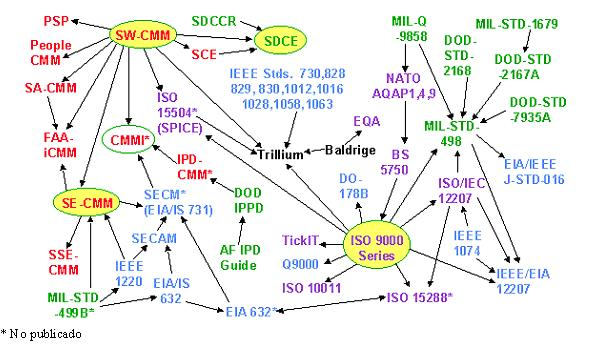
\includegraphics{./imagenes/marcostrabajo.jpg}
  \caption[\small Principales Marcos de Trabajo en el �rea de ingenier�a del software.]
 {\small Principales Marcos de Trabajo en el �rea de ingenier�a del software \cite{BED1998}.}
  \label{figmarcostrabajo}
\end{figure}

A continuaci�n se describen los m�s importantes.\\

\subsection{CMM�} \label{mtcmm}

Como se indic� en el apartado \ref{marcointroduccion}, el Capability Madurity Model (Modelo de Capacidad de Madurez) surgi� a ra�z de la crisis del software sufrida a principios de los a�os 80 y como encargo del Departamento de Defensa de los Estados Unidos al SEI de la Universidad Carnegie Mellon.\\

El principal autor del modelo es Watts Humphrey, quien trabaj� en la elaboraci�n del CMM basado en trabajos previos de Phil Crosby \cite{BAC1994}.\\

Este modelo se basa en dos conceptos importantes: el proceso maduro y el nivel de madurez.\\

Un proceso se considera maduro si \cite{SAL2000}:
\begin{itemize}
\item	Est� definido: es claro y detallado.
\item	Est� documentado.
\item	El personal ha sido entrenado en el proceso.
\item	Es mantenido: es revisado regularmente.
\item	Est� controlado: cualquier cambio es revisado y comunicado a todo el personal.
\item	Se verifica: es claro si el proceso est� envuelto en todos los proyectos actuales o no.
\item	Se valida: el proceso es coherente con los requerimientos y est�ndares.
\item	Se mide en t�rminos de beneficio, utilizaci�n y rendimiento.
\item	Es mejorable.
\end{itemize}

La figura \ref{figmaduracionproceso} muestra la manera en que un proceso alcanza la madurez deseada por una empresa.\\

\begin{figure}[!ht]
  \centering
  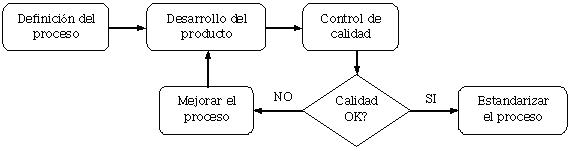
\includegraphics{./imagenes/maduracionproceso.jpg}
  \caption[\small Maduraci�n de un proceso]
  {\small Maduraci�n de un proceso \cite{BED1998}.}
  \label{figmaduracionproceso}
\end{figure}

El nivel de madurez est� definido como:

\begin{quote}
{\it ``La capacidad de los procesos de ingenier�a del software y de administraci�n de proyectos usados en una organizaci�n de desarrollo de software''} \cite{SAL2000}. 
\end{quote}

La capacidad de los procesos en conjunto est� determinada por la madurez de cada uno de ellos.\\

A su vez, el CMM� envuelve toda una familia de sub-modelos, cada uno de los cuales se enfoca en un �rea espec�fica de la empresa. De esta manera se tienen \cite{SAL2000}:
\begin{itemize}
\item	SW-CMM (Software CMM): Aplicado espec�ficamente al �mbito del software.
\item	SE-CMM: (Systems Engineering CMM): Que cubre el �mbito de la Ingenier�a de Sistemas propiamente dicha.
\item	P-CMM (Personal CMM): Se enfoca en los recursos humanos de la organizaci�n.
\item	SA-CMM (Software Acquisition CMM): El cual cubre las pr�cticas de adquisici�n de productos de software. Aunque suene ir�nico, es la actividad inevitable de las empresas de desarrollo de software; todas en determinado momento adquieren productos hechos por otras empresas a fin de poder desarrollar los propios.
\item	IPD-CMM (Integrated Product Development CMM): Aplicado al �mbito de la integraci�n del producto.
\end{itemize}

El CMM� clasifica a las empresas involucradas en el desarrollo de software en cinco niveles de acuerdo a los criterios que maneja (la madurez de sus procesos y la calidad de los resultados que se obtienen de esos procesos). Entonces se tiene:\\

{\bfseries - Nivel 1: Inicial (Inmadurez) }\\

Tambi�n conocido como el ``Nivel del Caos''. Aqu� se encuentran todas las empresas que no han logrado implementar pr�cticas b�sicas de Ingenier�a del software y donde el personal coincide en que los proyectos no se pueden planear y los requerimientos se salen de control. Por lo general, la conclusi�n de un proyecto se logra a coste de muchas horas extra de trabajo y con una inversi�n injustificada \cite{SAL2000}.\\

{\bfseries - Nivel 2: Repetible (El proyecto planificado)}\\

Este nivel se caracteriza por la presencia en las empresas de pr�cticas m�nimas de Ingenier�a del software y donde la experiencia adquirida en proyectos anteriores es bien aprovechada por el personal. En este punto, no necesariamente todos los procesos tienen el mismo nivel de madurez \cite{SAL2000}.\\

El mayor beneficio de este nivel es la planificaci�n realista de los proyectos, la cual en general no expresa el deseo de la gerencia, factor que en el nivel 1 es el principal determinante para las malas estimaciones \cite{SAL2000}.\\

{\bfseries - Nivel 3: El proceso definido (El proceso generalizado en todos los proyectos)}\\

Para llegar a este nivel, la empresa tiene bien definido un conjunto de procesos y herramientas comunes a todos los proyectos. Cada proceso est� debidamente documentado y el personal est� entrenado en el manejo del mismo. El nivel de definici�n de cada proceso es detallado y completo. La dependencia en individuos ``irreemplazables'' es baja, al contrario que en los dos anteriores niveles\cite{SAL2000}.\\

Una caracter�stica notoria del nivel 3 es la satisfacci�n del personal. Por lo general en las empresas del nivel 1 y algunas del 2 las quejas, acusaciones y frustraci�n en el personal son caracter�sticas siempre presentes debido a los fracasos que acarrea la falta de aplicaci�n de pr�cticas formales de ingenier�a del software y administraci�n de proyectos.\\

Llegar a este nivel es considerado para muchos un lujo.\\

{\bfseries - Nivel 4: El proceso gestionado}\\

En este nivel, tanto el proceso como el producto son cuidadosamente controlados mediante m�tricas precisas. Sin embargo, contar con un conjunto de m�tricas no significa necesariamente que la empresa pueda ser calificada en este nivel \cite{SAL2000}.\\

La ventaja con la que cuentan las empresas del nivel 4 es la capacidad que tienen de poder medir su productividad y calidad; la capacidad de rendimiento de un proceso es previsible.\\

{\bfseries - Nivel 5: Mejoramiento permanente}\\

Este nivel, denominado tambi�n ``ut�pico'' por algunos expertos, se basa en la realimentaci�n cuantitativa e implementaci�n de tecnolog�as innovadoras en la empresa. La organizaci�n entera se enfoca en el mejoramiento continuo de sus procesos\cite{SAL2000}.\\

El �ltimo es considerado el nivel ideal pero pr�cticamente inalcanzable debido al nivel de madurez que se debe alcanzar. Tan s�lo una veintena de empresas en todo el mundo han conseguido calificar en este nivel.\\

La figura \ref{fignivelescmm} muestra a manera de esquema los niveles de madurez de CMM.\\

\begin{figure}[!ht]
  \centering
  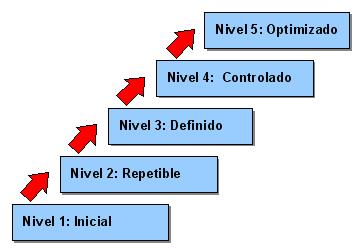
\includegraphics{./imagenes/nivelescmm.jpg}
  \caption[\small Niveles de madurez seg�n el CMM]
  {\small Niveles de madurez seg�n el CMM \cite{PIC2003}.}
  \label{fignivelescmm}
\end{figure}
 
La figura \ref{figempresascmm} muestra la relaci�n entre las empresas de software certificadas y los niveles del CMM�. Se destaca en el gr�fico que la cantidad de empresas disminuye de forma considerable a medida que se sube de nivel, lo cual demuestra el enorme esfuerzo que se requiere para poder obtener una certificaci�n aceptable (a partir del nivel 3). El detalle de las empresas certificadas por este modelo se encuentra en el Anexo \ref{anexocertificaciones}.\\
 
\begin{figure}[!ht]
  \centering
  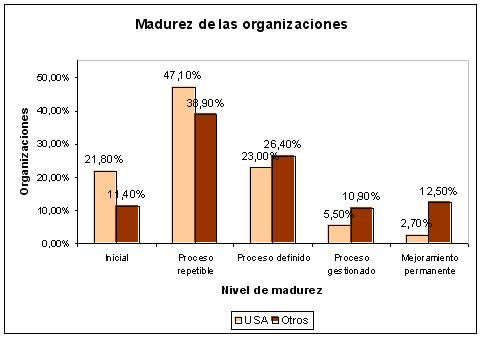
\includegraphics{./imagenes/empresascmm.jpg}
  \caption[\small Nivel de madurez de las organizaciones en todo el mundo seg�n el CMM�]
  {\small Nivel de madurez de las organizaciones en todo el mundo seg�n el CMM� (a septiembre de 2003) \cite{SEI2003}.}
  \label{figempresascmm}
\end{figure}

\clearpage
{\bfseries Desventajas}\\

Este modelo ayud� a sacar a las empresas de desarrollo de software de la mencionada crisis en la que se vieron inmersas a inicios de los a�os 80 y plante� una nueva concepci�n del desarrollo de software al introducir el concepto de que la calidad de un producto depende del nivel de madurez de los procesos que est�n involucrados en su desarrollo. Sin embargo, es un modelo muy inflexible, existen empresas que no califican en ning�n nivel y otras que pueden perder su certificaci�n o bajar de nivel si alguno de sus procesos desmejora.\\

Adem�s de esta inflexibilidad, CMM� es criticado por algunos expertos, como James Bach de la Satisfice Inc. quien en su art�culo ``The Immaturity of CMM'' (La Inmadurez del CMM) asegura que este modelo posee entre otras, las siguientes falencias \cite{BAC1994}:

\begin{itemize}
\item	No posee bases te�ricas formales, sino que simplemente est� basado en la ``extensa experiencia de la gente''. De ser as�, entonces se plantea la inc�gnita de porqu� otros modelos fundados sobre las mismas bases no son considerados como alternativas v�lidas.
\item	El modelo posee un vago soporte emp�rico. Incluso Mark Paul del SEI reconoce que al modelo le falta un serio estudio de validaci�n formal.
\item	CMM� valora cualquier proceso, pero ignora a la gente.
\item	CMM� proporciona muy poca informaci�n referente a la din�mica de los procesos, es decir, la manera en que estos trabajan y evolucionan.
\item	El modelo desplaza las metas que se enfocan en mejorar los procesos por la �nica finalidad de alcanzar un nivel m�s alto de madurez. A esto se le ha denominado el ``nivel de envidia''. Es decir, las empresas se ciegan en busca de un ascenso de nivel perdiendo por completo el verdadero sentido de aplicar el CMM�: la mejora de sus procesos. El mismo SEI ha reconocido esta falencia y ha manifestado su deseo de corregirla.
\end{itemize}

Dadas estas debilidades del modelo y puesto que en general las empresas nacionales no est�n preparadas para una certificaci�n tan severa, no es recomendable considerar (por lo menos ahora) el CMM� como un modelo base para el inicio de implementaci�n de t�cnicas formales de control de calidad en las empresas locales.\\

\subsection{ISO}

Esta organizaci�n certifica a las empresas mediante sus est�ndares 8402, 9000, 9001, 9002, 9003 y 9004, que han sido desarrollados desde 1979. Estos est�ndares imponen una serie de normas y directrices que deben ser seguidas por las empresas para conseguir la certificaci�n \cite{BUA2000} \cite{GON1998}:\\

El primero (ISO-8420) se refiere solamente a la terminolog�a utilizada en los dem�s est�ndares \cite{BUA2000}.\\

ISO-9000 establece las normas referentes a la gesti�n y garant�a de la calidad as� como tambi�n algunas gu�as �tiles para la aplicaci�n de ISO-9001; es una gu�a b�sica de normas de control de calidad \cite{TEC2003}.\\

En este est�ndar, ISO trata a las empresas como redes de procesos interconectados. �stos deben ser identificados en �reas espec�ficas definidas en los est�ndares y ser documentados y practicados como lo indica la especificaci�n \cite{PRE2002}.\\

ISO-9001 es el est�ndar que se aplica a la Ingenier�a del Software y que otorga la garant�a de calidad total. Este est�ndar est� asociado a un conjunto de directrices para ayudar a las empresas en la interpretaci�n y uso correcto del est�ndar. Estas directrices est�n especificadas en los est�ndares ISO-9000-3 \cite{PRE2002}.\\

ISO-9002 a ISO-9003 establecen las normas y gu�as que conforman en modelo de calidad total, como ya se indic� l�neas arriba \cite{BUA2000} \cite{TEC2003}.\\

ISO-9004 contiene elementos de gesti�n del sistema de calidad, reglas generales y directrices para los elementos ya procesados y la mejora de la calidad \cite{BUA2000}.\\

B�sicamente estas normas establecen la misma secuencia descrita en el apartado \ref{marcostrabajo} (un conjunto de actividades para cada fase del desarrollo del producto).\\

La lista de empresas certificadas por ISO se encuentra en el Anexo \ref{anexocertificaciones}.\\

\subsection{SPICE}

An�logo al CMM, el Software Process Improvement and Capability dEtermination es un  modelo enfocado en la optimizaci�n (maduraci�n) de los procesos que son utilizados en el desarrollo de software.\\

SPICE, en calidad de proyecto, fue aprobado por la ISO/IEC JTC1 en 1993 y tiene la finalidad de convertirse en un est�ndar de calidad llamado ISO/IEC 15504. Es un modelo de referencia para los procesos y sus capacidades, basado en la experiencias de empresas de software de distinta escala \cite{BED1997}.\\

Entre los documentos de gu�a que ofrece, se encuentran \cite{BED1997}:
\begin{itemize}
\item	Un marco de referencia para determinar las fortalezas y debilidades de cada proceso.
\item	Un marco de referencia para la mejora de los procesos de software y la cuantificaci�n de la misma.
\item	Un marco de referencia para determinar los riesgos a los que se ve expuesto una empresa que planea desarrollar un nuevo producto de software.
\end{itemize}

La arquitectura del modelo SPICE organiza todas las actividades en \cite{BED1997}:
\begin{itemize}
\item	Pr�cticas base o actividades esenciales para cada proceso.
\item	Pr�cticas gen�ricas: las que son aplicables a cualquier proceso.
\end{itemize}

A su vez, el modelo agrupa a los procesos en cinco categor�as distintas \cite{BED1997}:
\begin{itemize}
\item	Procesos Cliente - Proveedor: aquellos que tienen un impacto directo en el cliente y en la transici�n del producto del desarrollador al cliente.
\item	Procesos de Ingenier�a: procesos relacionados con la Ingenier�a del Software (planificaci�n, desarrollo, documentaci�n, mantenimiento, etc.).
\item	Procesos de Proyecto: aquellos involucrados en la elaboraci�n del producto, como la administraci�n de los recursos.
\item	Procesos de Soporte: se refiere a los procesos orientados a brindar soporte al desempe�o de otros procesos del proyecto.
\item	Procesos de la Organizaci�n: propios a la organizaci�n. Son los procesos que determinan las metas de negocio de una empresa.
\end{itemize}

La figura \ref{figprocesosspice} ilustra la interrelaci�n que existe entre las cinco categor�as mencionadas.

\begin{figure}[!ht]
  \centering
  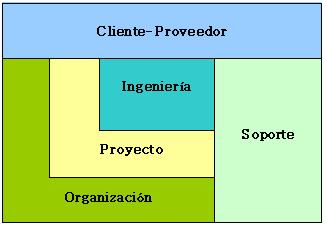
\includegraphics{./imagenes/procesosspice.jpg}
  \caption[\small Interrelaci�n de las categor�as de procesos seg�n SPICE]
  {\small Interrelaci�n de las categor�as de procesos seg�n SPICE \cite{BED1997}.}
  \label{figprocesosspice}
\end{figure}

Dependiendo de la madurez de los procesos de estas cinco categor�as, una empresa puede ubicarse en uno de los seis niveles de SPICE \cite{BED1997}:\\

{\bfseries -	Nivel 0: No realizado}\\

En este nivel se clasifican las empresas que no han conseguido la implementaci�n satisfactoria de sus procesos.\\

{\bfseries -	Nivel 1: Realizado informalmente}\\

Las empresas de este nivel ejecutan las pr�cticas base de sus procesos pero no necesariamente de manera planificada y sistem�tica. Es decir, la ejecuci�n de estas pr�cticas depende directamente del esfuerzo y conocimiento del personal.\\

{\bfseries -	Nivel 2: Planificado y seguido}\\

A diferencia del Nivel 1, las pr�cticas base de las empresas de este nivel son planificadas y sistem�ticas, lo que contribuye a una mejora progresiva del proceso que concluir� en la madurez del mismo.\\

{\bfseries -	Nivel 3: Bien definido}\\

En este nivel se clasifican las empresas cuyos procesos cuentan con un grado aceptable de madurez, es decir, son procesos definidos y documentados.\\

{\bfseries -	Nivel 4: Cuantitativamente controlado}\\

En este nivel, los procesos adem�s de estar definidos y documentados, son medibles en t�rminos de los resultados que producen al ser utilizados en un proyecto.\\

{\bfseries -	Nivel 5: Mejoramiento continuo}\\

Las empresas de este nivel cuentan con procesos maduros cuyo mejoramiento permanente se basa en la retroalimentaci�n y en la implantaci�n de nuevas tecnolog�as.\\

La figura \ref{fignivelesspice} miestra el esquema de los seis niveles SPICE.

\begin{figure}[!ht]
  \centering
  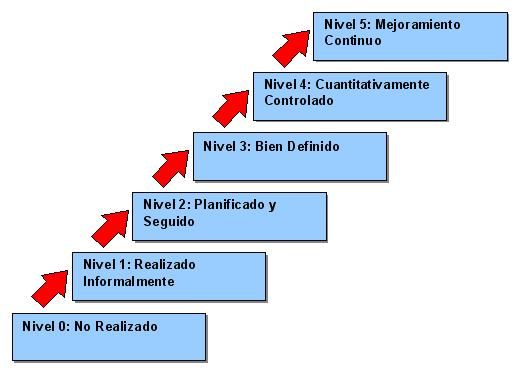
\includegraphics{./imagenes/nivelesspice.jpg}
  \caption[\small Niveles de madurez seg�n SPICE]
  {\small Niveles de madurez seg�n SPICE \cite{PIC2003}.}
  \label{fignivelesspice}
\end{figure}

\subsection{IEEE}

El Institute of Electrical and Electronics Engineers certifica a las empresas que cumplen con los requisitos que plantea, tal como lo hace el ISO y el CMM�. Estos requisitos se encuentran documentados en los siguientes est�ndares:
\begin{itemize}
\item	IEEE 828-1998: est�ndar para la configuraci�n de planes de administraci�n del software, que establece los requisitos m�nimos con los que debe contar el Plan de Configuraci�n y Administraci�n del Software \cite{TEC2003}.
\item	IEEE 1012-1998: un est�ndar para la verificaci�n y validaci�n del software, que consiste en la determinaci�n de qu� actividades involucradas en el desarrollo del mismo cumplen con los requisitos m�nimos necesarios para ejecutarlas correctamente y si el producto final satisface las necesidades del usuario \cite{TEC2003}.
\end{itemize}

Para complementar esta secci�n, se incluyen los siguientes apartados (que no corresponden a los MT):

\subsection[Teor�a del ``Planear, hacer, revisar y actuar'']
{Teor�a del ``Planear, hacer, revisar y actuar'' (Plan, do, check, act)} \label{plandocheckact}

Esta teor�a se basa en los cuatro puntos mencionados:
\begin{itemize}
\item	Planear: consiste en la etapa de planificaci�n de los casos de prueba.
\item	Hacer: en esta fase se elaboran los casos de prueba.
\item	Revisar: es una evaluaci�n previa de los casos dise�ados antes de su ejecuci�n.
\item	Actuar: consiste en la ejecuci�n de los planes de testeo planificados anteriormente.
\end{itemize}

Estas tareas son realizadas en un ciclo permanente. Una vez terminada la fase de ``actuar'', se procede nuevamente a la de planear. Estas actividades son realizadas a lo largo de todo el proceso de desarrollo del software \cite{LEW2000}.

\subsection{Otros}

Como las propuestas presentadas en este apartado, existen otros modelos y est�ndares menos conocidos pero �tiles y que son aplicados en algunas empresas, como es el caso del Modelo McCall \cite{CER2000}.\\

No existe un modelo perfecto, ninguno se acomoda al cien por ciento a las necesidades de una empresa y mucho menos garantiza ser la soluci�n a sus problemas de calidad. Cada modelo plantea un objetivo ideal y com�n, que debe ser moldeado de acuerdo a los problemas que se presenten en la organizaci�n.

\begin{quote}
{\it ``Todos los modelos son err�neos; algunos modelos son �tiles''}
George Box. \cite{GAR2001}.
\end{quote}

\section{El costo de la calidad} \label{costocalidad}

La implementaci�n de metodolog�as de control de calidad en una empresa acarrea su propio costo, que por lo general es elevado. Sin embargo, al ser pr�cticas que pretenden mejorar el rendimiento de los recursos invertidos, este costo resulta ser mucho menor al que la empresa asume cuando se trata de reparar fallas graves detectadas en las �ltimas fases del desarrollo o, aun peor, las reportadas por los clientes.\\

Estos costos est�n asociados con la prevenci�n, la evaluaci�n y la correcci�n de fallas.\\

Los costos de prevenci�n involucran:
\begin{itemize}
\item	Planificaci�n de la calidad.
\item	Revisiones t�cnicas.
\item	Equipo de pruebas.
\item	Formaci�n (capacitaci�n).
\end{itemize}

Los costos de evaluaci�n son los resultantes de las inspecciones en los procesos, el mantenimiento de equipos y las pruebas.\\

Finalmente, los costos de fallos son aquellos que no existir�an si el producto final careciera de defectos. Estos costos pueden ser internos si los defectos son detectados antes de la entrega del producto y externos si son reportados por los clientes una vez que el producto ha sido entregado.\\

Los costos internos incluyen los costos de revisi�n y reparaci�n.\\

En el caso de los fallos externos los costos se elevan puesto que implican adem�s de las reparaciones, los costos de la devoluci�n y sustituci�n de los productos.\\

Los costos de fallos se elevan a medida que el proyecto llega a sus �ltimas fases. Estudios realizados en base a experiencias de empresas como IBM demuestran este hecho \cite{PRE2002}.\\

{\bfseries Impacto de los defectos del software sobre el costo}\\

Una serie de estudios realizados por empresas como Nippon Electric y Mitre Corp. demostr� que entre el 50 y 65 por ciento del total de errores se producen durante la etapa del dise�o y que las actividades de revisi�n formales son efectivas en un 75 por ciento a la hora de detectar estos errores, lo que reduce sustancialmente el costo en los pasos siguientes \cite{PRE2002}.\\

La figura \ref{figcostocalidad} muestra el resultado de estos estudios (incluido el realizado a IBM), demostrando las proporciones del costo de arrastrar un error hasta las �ltimas fases.

\begin{figure}[!ht]
  \centering
  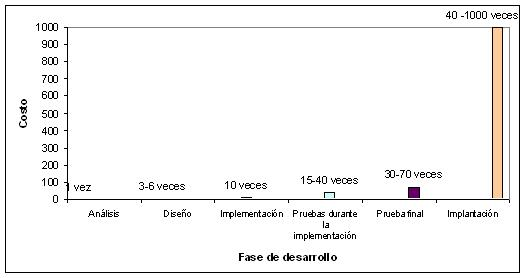
\includegraphics{./imagenes/costocalidad.jpg}
  \caption[\small Costo relativo de corregir un error]
  {\small Costo relativo de corregir un error \cite{PRE2002}.}
  \label{figcostocalidad}
\end{figure}
 
\section{Los beneficios de la calidad}

Al tiempo que la implementaci�n de m�todos de control de calidad ayuda a mitigar (o en el mejor de los casos a eliminar por completo) los problemas descritos en apartados anteriores, la presencia de procesos maduros y pr�cticas de calidad formales en una empresa proporciona, entre otros, los siguientes beneficios \cite{ASQ2003}:
\begin{itemize}
\item	En los empleados: la satisfacci�n de efectuar un buen trabajo, la mejora de la comunicaci�n interna, una mejor organizaci�n del personal, la reducci�n e incluso eliminaci�n de la necesidad de realizar esfuerzos extra para terminar un proyecto.
\item	En la empresa: el uso eficiente de los recursos, la reducci�n de costos, la garant�a de realizar buenas estimaciones, la seguridad de obtener resultados positivos al finalizar un proyecto.
\item	En los clientes: la confianza de que el producto adquirido satisface sus necesidades.
\item	En la sociedad: el crecimiento de la industria del software, lo que permite abrir el mercado y atraer a clientes tanto nacionales como internacionales y la reducci�n de la dependencia por el software externo.
\end{itemize}

\chapter{ASEGURAMIENTO DE LA CALIDAD DEL SOFTWARE}

El Aseguramiento de la Calidad del Software (Software Quality Assurance, SQA) es el conjunto de actividades planificadas y sistem�ticas necesarias para aportar la confianza de que el producto de software cumplir� con los requisitos dados de calidad. Es dise�ado antes del desarrollo del proyecto y est� presente en:
\begin{itemize}
\item	M�todos y herramientas (de an�lisis, dise�o, implementaci�n y pruebas).
\item	Inspecciones t�cnicas formales en todos los pasos del proceso de desarrollo del producto.
\item	Estrategias de prueba.
\item	Control de la documentaci�n del software y de los cambios realizados en el mismo.
\item	Procedimientos que permiten ajustarse a los est�ndares de calidad.
\item	M�tricas.
\item	Informes realizados por las personas involucradas en el desarrollo (analistas, desarrolladores, testers, etc.).
\end{itemize}

Las actividades de las que el SQA est� conformado son b�sicamente:
\begin{itemize}
\item	Verificaci�n y validaci�n: la verificaci�n es la actividad encargada de evaluar si el producto cumple con el desarrollo planificado (``se est� construyendo adecuadamente'') mientras que la validaci�n comprueba si el software que se est� construyendo es el correcto para las necesidades planteadas (``se est� construyendo el adecuado''). Ambas tareas van de la mano y se aplican  en cada fase del desarrollo \cite{LEW2000} \cite{GER2003}.
\item	Gesti�n de la configuraci�n del software.
\end{itemize}

\section{Actividades del SQA}

SQA abarca una amplia gama de actividades asociadas tanto a los desarrolladores como al propio equipo de calidad de la empresa.\\

El equipo de desarrolladores es responsable de aplicar m�todos planificados y t�cnicas de revisi�n formales durante su trabajo. El equipo de SQA intenta ayudar al primero en la obtenci�n de un software de alta calidad mediante la aplicaci�n de t�cnicas de SQA como \cite{PRE2002}:
\begin{itemize}
\item	Establecimiento de un plan de SQA para cada proyecto, el mismo que es revisado por todo el personal involucrado. Rige todas las actividades de ambos equipos. El plan define criterios como:
	\begin{itemize}
	\item	Las evaluaciones a realizar.
	\item	Los est�ndares a aplicar.
	\item	Los procedimientos a seguir para la documentaci�n de los errores.
	\item	El {\it feedback} del proyecto.
\end{itemize}
\item	Participaci�n en el desarrollo de la descripci�n del proceso de software en el proyecto.
\item	Revisi�n de las actividades de ingenier�a del software para verificar que se ajusten al proceso de software definido.
\item	Asegurar que las desviaciones del trabajo y los productos se documenten y manejen de acuerdo con un procedimiento establecido.
\item	Registrar lo que no se ajuste a los requisitos e informar a los supervisores.
\end{itemize}

{\bfseries Revisiones T�cnicas Formales}\\

Una Revisi�n T�cnica Formal (RTF) es una actividad de SQA que es llevada a cabo por los ingenieros del software y que pretende alcanzar los siguientes objetivos:
\begin{itemize}
\item	Descubrir errores durante el desarrollo.
\item	Verificar que el software cumpla con sus requisitos.
\item	Verificar que el software cumpla con los est�ndares establecidos.
\item	Hacer que los proyectos sean manejables.
\item	Conseguir un desarrollo uniforme del proyecto.
\end{itemize}

Adem�s de esto, una RTF permite promover la seguridad y continuidad permitiendo que todas las personas involucradas se familiaricen con todas las partes del software (ya que puede darse el caso en que una o m�s personas ignoren algunas) \cite{PRE2002}.\\

Una RTF viene acompa�ada de las reuniones de revisi�n, donde tanto desarrolladores como ingenieros de calidad se concentran en la revisi�n de una etapa completa del desarrollo del producto o, si la complejidad lo amerita, en la etapa de desarrollo de un determinado m�dulo. Por ejemplo, una reuni�n puede estar destinada a la revisi�n del dise�o de un solo m�dulo del sistema \cite{PRE2002}.\\

Es en estas reuniones (denominadas tambi�n por algunos ``War Meetings''\footnote{Extra�do de la charla de Dr. Pavisic: ``T�picos de ingenier�a del software'' que tuvo lugar en mayo de 2003 en la Universidad Cat�lica Boliviana, Regional Cochabamba.}) donde los ingenieros de calidad y los desarrolladores deciden qu� errores se corrigen y cu�les se omiten moment�neamente, puesto que existen errores cuya severidad no amerita la inversi�n de tiempo que requiere su reparaci�n y mucho menos la postergaci�n de otras tareas m�s importantes para  concentrar al personal en resolverlo. Si bien el objetivo de estas reuniones es reducir al m�ximo la cantidad de errores que se encuentren, tambi�n debe haber un balance porque de todas formas siempre existir�n defectos y la tarea de eliminarlos puede convertirse en algo eterno y a la larga perjudicial para la empresa.\\

Es necesario que todo el personal involucrado est� consciente de que el software perfecto no existe y que lo que se busca es que el producto final tenga la menor cantidad de defectos posible sin invertir m�s recursos de los destinados al proyecto.

\section{SQA en las distintas fases del desarrollo}

Como se dijo anteriormente, el control de calidad es una tarea que se realiza a lo largo de todo el proceso de desarrollo del producto de software. Es as� que para cada fase de este proceso se tienen algunas consideraciones.\\

{\bfseries Herramientas}\\

Para un efectivo control de calidad durante todas las fases del desarrollo, existen herramientas bastante recomendables. Algunas de ellas se describen a continuaci�n:\\

\begin{itemize}

\item	{\bfseries Inspecciones}\\\\
Esta es una t�cnica utilizada para evaluar permanentemente el avance de la documentaci�n, el cumplimiento de los requerimientos y el apremio de la soluci�n \cite{LEW2000}.

\item {\bfseries Casos de Prueba}\\\\
Son una herramienta bastante efectiva y com�n. Cada caso consta de especificaciones que el tester debe seguir para realizar una prueba espec�fica sobre una funcionalidad determinada del sistema. Una vez hecha la prueba, se determina si el caso pas� o fall�. De ocurrir lo �ltimo, se registra el defecto y se comunica el resultado al desarrollador para que �ste haga las correcciones debidas.\\

Un modelo de caso de prueba se presenta en el Anexo \ref{anexocasospruebachecklists}.

\item {\bfseries Listas de Control}\\\\
M�s conocidas como {\it Checklists}, constan de una serie de preguntas que tienen como objetivo asegurar que tanto los requerimientos como la metodolog�a se est�n cumpliendo.\\

Cada defecto que sea detectado mediante estas listas debe ser documentado \cite{LEW2000}.\\

Tanto para la elaboraci�n del checklist como para la documentaci�n de los defectos, se propone la utilizaci�n de herramientas como la que se muestran en el Anexo \ref{anexocasospruebachecklists}, que combinan ambos reportes en uno solo.

\item {\bfseries 	Matriz de seguimiento de requisitos}\\\\
Una matriz de seguimiento de requisitos es un documento que sirve para hacer un control de los requerimientos del software desde la etapa de an�lisis hasta la de implementaci�n. Es utilizada para verificar que ning�n requisito se haya ``perdido'' en el camino, que no existan caracter�sticas innecesarias y que la documentaci�n est� completa \cite{LEW2000}.

\item {\bfseries Plan de Testeo}\\\\
Este documento, basado en el de especificaci�n de requerimientos, se elabora durante todas las fases para verificar que el sistema cumple con los criterios de aceptaci�n del usuario \cite{LEW2000}.\\

Un modelo de este documento es presentado en el Anexo \ref{anexoespecificacionrequerimientos}.
\end{itemize}


{\bfseries a)	Fase de requerimientos}\\

El control de calidad debe comenzar desde las fases m�s tempranas del desarrollo, no s�lo durante la tradicional fase de pruebas donde pueden aparecer errores cuyo costo (en recursos humanos, tiempo y dinero) es elevado y puede evitarse si tales errores son detectados en fases previas.\\

�sta es quiz� la fase m�s importante en t�rminos de calidad ya que durante las dem�s fases del desarrollo se busca que los requerimientos se cumplan; por lo tanto, malos requerimientos derivar�n en un mal producto.\\

Los requerimientos pobres incluyen \cite{LEW2000}:
\begin{itemize}
\item	Funciones parcialmente definidas.
\item	Omisi�n del performance.
\item	Requerimientos ambiguos, contradictorios o redundantes.
\item Interfaces no documentadas.
\item	Requerimientos demasiado restrictivos (inflexibles).
\end{itemize}

Las secciones m�s importantes en una especificaci�n son \cite{LEW2000}:
\begin{itemize}
\item	Funcionalidad: el conjunto de tareas que el sistema debe ser capaz de realizar.
\item	Descripci�n de los datos.
\item	Descripci�n de las interfaces entre la funci�n y las entidades externas.
\end{itemize}

Un modelo del documento de especificaci�n de requerimientos se presenta en el Anexo \ref{anexoespecificacionrequerimientos}.\\


{\bfseries Plan de testeo - Prueba de aceptaci�n}\\

Para la ejecuci�n de esta prueba, se realiza un testeo de caja negra\footnote{Conjunto de pruebas donde lo �nico que interesa es verificar la funcionalidad y no as� la manera en que el programa ejecuta las tareas.} y, por lo general, es el usuario final quien participa activamente de ella. Naturalmente, se espera que para hacer este tipo de testeo el producto est� implementado o por lo menos una parte de �l, lo que implica que el equipo de desarrollo se encuentre trabajando en las �ltimas fases. aun as� es importante comenzar la construcci�n de esta prueba desde la fase de requerimientos y que el usuario eval�e si sus requerimientos se est�n cumpliendo o no \cite{LEW2000}.\\

Una herramienta que facilita la ejecuci�n de esta prueba es la Matriz de Testeo de Especificaciones, que se muestra a manera de ejemplo en la figura \ref{figmatriztesteo}. Adem�s, esta matriz presenta beneficios adicionales como \cite{LEW2000}:
\begin{itemize}
\item	Permite establecer una correlaci�n entre las pruebas y la documentaci�n y los requisitos.
\item	Facilita el mantenimiento de los documentos de revisi�n.
\item	Es una herramienta que permite el seguimiento del desarrollo durante todas las etapas del mismo, incluyendo la implantaci�n.
\end{itemize}
 
\begin{figure}[!ht]
  \centering
  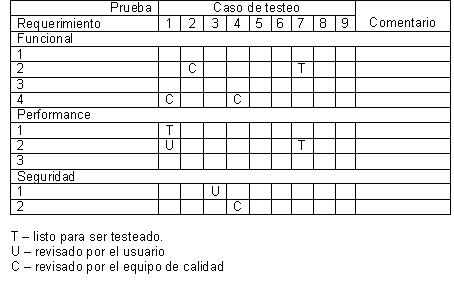
\includegraphics{./imagenes/matriztesteo.jpg}
  \caption[\small Matriz de testeo de especificaciones]
  {\small Matriz de testeo de especificaciones \cite{LEW2000}.}
  \label{figmatriztesteo}
\end{figure}

{\bfseries b)	Fase de Dise�o}\\
	
�sta es quiz� la etapa que se encuentra m�s comprometida con la calidad del producto porque su resultado ser� la base para la implementaci�n. Pr�cticamente todo diagrama, esquema o documento resultante de esta fase ser� convertido en c�digo por los programadores, por lo que se debe hacer todo lo posible para que �stos carezcan de errores.\\

Se sabe que del 50 al 65 por ciento de los errores que se detectan en los productos de software provienen de su dise�o, por lo que dedicar un �nfasis especial a esta etapa puede garantizar una reducci�n (m�s adelante) del esfuerzo que se emplea para corregir los defectos que aparecer�n \cite{PRE2002}.\\

En el apartado \ref{costocalidad} se explica adem�s porqu� a nivel econ�mico es importante evitar el acarreo de los defectos que aparecen en las fases tempranas.\\

Esta fase se divide en tres: el dise�o l�gico, el dise�o f�sico y el dise�o de unidad de la aplicaci�n.\\

{\bfseries b.1)	Evaluaci�n de la fase de Dise�o L�gico}\\

Esta fase especifica lo dicho en los requerimientos funcionales, los requisitos que tienen que ver directamente con la l�gica del negocio.\\

El dise�o l�gico de una aplicaci�n establece un marco de trabajo (framework) detallado para la construcci�n del sistema. Los tres conceptos m�s importantes de este framework son el modelo de datos, el modelo del proceso y el enlace entre ambos \cite{LEW2000}.\\

El modelo de datos es una representaci�n de la informaci�n (el tipo de cada uno de los datos involucrados) necesaria para la aplicaci�n. Permite definir tanto las entidades como las relaciones presentes en la aplicaci�n \cite{LEW2000}.\\

El modelo del proceso es una descomposici�n del negocio, es decir,  es el desglose detallado de las actividades involucradas, desde su nivel m�s abstracto hasta el m�s elemental.\\	

El enlace entre ambos modelos se realiza mediante una representaci�n gr�fica de toda la l�gica del negocio. Una de las t�cnicas para esta representaci�n es la Matriz CRUD (para el detalle de c�mo funciona consultar el Anexo D). Esta t�cnica puede ser adem�s utilizada con fines de testeo, utilizando su l�gica para formular una tabla como la que se muestra en la figura \ref{figmatrizcrud}.\\

\begin{figure}[!ht]
  \centering
  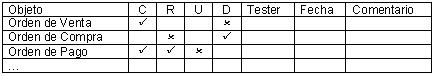
\includegraphics{./imagenes/matrizcrud.jpg}
  \caption[\small Matriz CRUD para el testeo]
  {\small Matriz CRUD para el testeo \cite{LEW2000}.}
  \label{figmatrizcrud}
\end{figure}

{\bfseries Plan de testeo - Prueba del sistema}\\

En esta secci�n se prosigue con la elaboraci�n del plan de prueba de aceptaci�n que se inici� en la fase anterior.\\

En esta fase se verifica que la l�gica de la aplicaci�n responda a los requisitos dados.\\

Para facilitar su ejecuci�n, se pueden utilizar herramientas como la propuesta para la fase de requerimientos (figura \ref{figmatriztesteo}) \cite{LEW2000}.\\


{\bfseries b.2)	Evaluaci�n de la fase de Dise�o F�sico}\\

Esta fase especifica la manera en que los requerimientos pueden ser automatizados, es decir, en esta etapa se dise�a la arquitectura del sistema.\\

Mientras que el dise�o l�gico es funcional, el dise�o f�sico es estructural y depende directamente del primero; por lo tanto, para esta fase, se asume que el dise�o l�gico es correcto. Algunas t�cnicas utilizadas para su representaci�n son los denominados Charts y los Diagramas de Flujo de Datos (consultar Anexo D para su detalle). Estos esquemas proveen mecanismos para la especificaci�n de los algoritmos a utilizar en algunos m�dulos del sistema. Es muy probable la presencia de inconsistencias en esta fase, sobretodo en la especificaci�n del flujo de la informaci�n entre los m�dulos \cite{LEW2000}.\\

{\bfseries Plan de testeo - Prueba de integraci�n}\\

El testeo en esta etapa se realiza mediante revisiones t�cnicas est�ticas, las cuales verifican que la arquitectura respete las convenciones establecidas, que el flujo de datos entre m�dulos no tenga inconsistencias y que la descomposici�n tanto de la informaci�n como de los procesos carezca de errores \cite{LEW2000}.\\

{\bfseries b.3)	Evaluaci�n de la fase de Dise�o de la Unidad del Programa}\\

Esta fase corresponde al dise�o detallado de la aplicaci�n en base a los dos dise�os anteriores y es donde los algoritmos y estructuras de datos son elegidos. Adem�s, especifica el flujo de control que har� que el dise�o sea f�cilmente traducible a un lenguaje de programaci�n espec�fico \cite{LEW2000}.\\

{\bfseries Plan de testeo - Prueba de Unidad}\\

El testeo en esta etapa es estrat�gico ya que es el �ltimo que se hace al dise�o antes de proceder a la implementaci�n. Si existen errores que no son corregidos, al ser traducidos a c�digo causar�n defectos importantes (incluso de grandes proporciones) que tarde o temprano ocasionar�n problemas al equipo de desarrollo y tiempos extra de implementaci�n para su correcci�n \cite{LEW2000}.\\

{\bfseries c)	Fase de Implementaci�n}\\

�sta es la fase donde el resultado del dise�o se traduce en c�digo de un determinado lenguaje de programaci�n; por lo tanto, depende enteramente de las decisiones que hayan sido tomadas previamente.\\

La traducci�n a un lenguaje de programaci�n es casi mec�nica si el dise�o es bueno. El desaf�o entonces para los programadores es garantizar que el c�digo producido sea robusto y f�cilmente mantenible a corto y largo plazo.\\

\clearpage
{\bfseries Plan de testeo - Conclusi�n}\\

El control de calidad en esta etapa se realiza mediante revisiones t�cnicas.\\
Todo lo efectuado en el plan de testeo durante las fases previas se completa en �sta. Para esto, en cada fase se debe elaborar un conjunto de casos de prueba que ser�n verificados cuando se termine la fase de implementaci�n \cite{LEW2000}.\\

{\bfseries d)	Fase de pruebas}\\

En esta secci�n se realizan todas las pruebas posibles al sistema. No solo se verifica que �ste cumpla con los requerimientos dados expl�citamente sino tambi�n con los impl�citos como la mantenibilidad, seguridad, exactitud, etc.\\


\section{SQA y la herramienta desarrollada}

Para el presente proyecto, se desarroll� una herramienta que, respondiendo a la teor�a de SQA:
\begin{itemize}
\item Permite la aplicaci�n de t�cnicas de control de calidad a trav�s de todo el proceso de desarrollo de software. Es decir, la ejecuci�n de pruebas en todas las fases del desarrollo.
\item Permite la ejecuci�n de algunas herramientas del SQA ya mencionadas: casos de prueba y listas de control.
\item	Permite la elaboraci�n de estrategias de prueba.
\item Permite el control de la documentaci�n del software y de los cambios realizados en el mismo (de manera b�sica).
\item	Permite la definici�n de procedimientos b�sicos que a la larga contribuyan en el ajuste a los est�ndares de calidad.
\item	Permite la aplicaci�n de m�tricas (expresadas en los casos de prueba y checklists) durante el control de calidad de los productos.
\end{itemize}

\chapter{M�TODOS Y HERRAMIENTAS}

\section{Modelo de arquitectura MVC}

La arquitectura MVC (Model View Controller) fue introducida como parte de la versi�n SmallTalk-80 del lenguaje de programaci�n SmallTalk. Fue concebida con el objetivo de reducir el esfuerzo que es invertido durante la implementaci�n de los sistemas m�ltiples y sincronizados con los mismos datos \cite{BUR1992}.\\

Como su nombre indica, posee tres partes esenciales: el Modelo, la Vista y el Controlador. Cada una es una entidad independiente, lo que permite \cite{BUR1992} \cite{APA2003}:
\begin{itemize}
\item	Establecer una clara separaci�n entre los componentes de la aplicaci�n, lo que a su vez permite implementarlos por separado.
\item	Hay un API bien definido; te�ricamente, si se lo utiliza no existe ning�n problema en hacer un reemplazo de cualquiera de las partes en cualquier momento.
\item	La conexi�n entre el View y el Model es din�mica, es decir, en tiempo de ejecuci�n.
\end{itemize}

\vspace*{0.3cm}
{\bfseries Modelo}\\

Encapsula la l�gica del negocio de la aplicaci�n. Es el objeto que representa los datos del sistema. Maneja la informaci�n y sus transformaciones. No posee ning�n conocimiento del Controlador o de la Vista y ni siquiera hace referencia a ellos (sobre este punto se detallar� m�s adelante) \cite{ANT1999} \cite{BUR1992} \cite{GOO2002}.\\

Internamente se divide en dos grandes subsistemas: Internal State (estado interno del sistema, de los objetos) y Actions, estas �ltimas son las que pueden cambiar al primero \cite{APA2003}.\\

Una analog�a clara que permite entender estos subsistemas es la de los objetos y los verbos en la gram�tica. En este caso el Internal State es el estado de cada uno de los objetos del sistema y los Actions son los verbos que son capaces de cambiar el estado de estos objetos \cite{APA2003}.\\

{\bfseries Vista}\\

Es el objeto encargado de manejar las vistas de la aplicaci�n. Genera una representaci�n visual para el usuario de la informaci�n recibida desde el Modelo, con el que interact�a mediante una referencia directa \cite{APA2003} \cite{GOO2002}.\\

{\bfseries Controlador}\\

Es la parte de la aplicaci�n que da sentido a las solicitudes del usuario. Todo el flujo de la aplicaci�n est� dirigido por �l. Es el encargado de delegar cada solicitud a un manejador apropiado. Estos manejadores est�n unidos a la entidad Modelo \cite{APA2003}.\\

Esta comunicaci�n entre las capas del modelo capas se encuentra ilustrado en la figura \ref{figmvc}.\\

\begin{figure}[!ht]
  \centering
  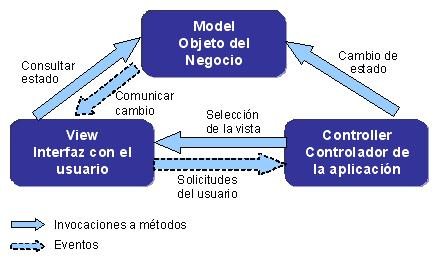
\includegraphics{./imagenes/mvc.jpg}
  \caption[\small Arquitectura MVC]{Arquitectura MVC \cite{ANT1999}.}
  \label{figmvc}
\end{figure}

\section{Metodolog�a}

Para el desarrollo de la ``Herramienta Web de apoyo al control de la calidad del software'', se utiliz� la metodolog�a RUP (Rational Unified Process).\\

Caracter�sticas del RUP \cite{IBA2003}: 
\begin{itemize}
\item	Es una gu�a que indica c�mo utilizar de manera efectiva el UML (Unified Modeling Language).
\item	Es una metodolog�a que envuelve una serie de pr�cticas utilizadas en el desarrollo moderno de software de una forma que es aplicable a una amplia gama de proyectos y organizaciones.
\item	Provee a cada miembro del equipo de desarrollo (analistas, dise�adores, desarrolladores, testers, etc.) un f�cil acceso a una base de conocimientos con gu�as y herramientas para todas las actividades cr�ticas de desarrollo.
\item	Crea y mantiene modelos que pueden ser aplicados en proyectos futuros en lugar de enfocarse en la producci�n de una gran cantidad de papeles de documentaci�n.
\end{itemize}

RUP describe adem�s la manera en que el equipo de desarrollo puede utilizar los procedimientos comerciales probados en el desarrollo de aplicaciones, conocidos como ``mejores pr�cticas'':
\begin{itemize}
\item	Administraci�n de requerimientos.
\item	Desarrollo iterativo.
\item	Modelamiento visual.
\item	Verificaci�n de calidad.
\item	Arquitectura de componentes.
\item	Control de cambios.
\end{itemize}

Con estas caracter�sticas, RUP ofrece un incremento en la productividad en el  trabajo tanto individual como grupal \cite{IBA2003}.\\

{\bfseries Fases en RUP}\\

RUP consta de cuatro fases \cite{IBA2003} \cite{RAM2001}:\\\\

{\bfseries 1. Inicio}\\

Su prop�sito es el de establecer los casos de negocio (casos de uso) para el nuevo sistema y el alcance del proyecto.\\

El resultado es una visi�n general de los requerimientos del proyecto y un caso de uso inicial que refleja la evaluaci�n inicial de riesgos y la estimaci�n de los recursos requeridos \cite{IBA2003}.\\

{\bfseries 2. Elaboraci�n}\\

Los objetivos de esta etapa son: el an�lisis del dominio del problema, el establecimiento de una buena arquitectura, el tratamiento de los elementos de riesgo m�s altos y la elaboraci�n de un plan donde se muestre c�mo el proyecto ser� finalizado \cite{IBA2003}.\\

Los resultados se muestran reflejados en: un modelo del dominio de casos de uso completado en un ochenta por ciento, una lista de requerimientos suplementarios que capturan los requerimientos no funcionales y otros que no est�n asociados con un caso de uso espec�fico y una lista de riesgos \cite{IBA2003}.\\

{\bfseries 3. Construcci�n}\\

En esta fase tiene lugar la implementaci�n del sistema.\\

Su resultado es el dise�o completo de la aplicaci�n, el producto desarrollado, la documentaci�n pertinente y una liberaci�n ``beta'' del producto \cite{IBA2003}.\\

{\bfseries 4. Transici�n}\\

En esta fase se transfiere el producto al usuario (aplicaci�n, manuales y documentaci�n) y se hace una evaluaci�n de los resultados midiendo el grado de satisfacci�n del usuario. Adem�s, se realiza una evaluaci�n interna en la empresa donde se determina si los gastos estimados resultaron siendo pr�ximos o no a los gastos reales \cite{IBA2003}.\\

La figura \ref{figfasesrup} muestra la distribuci�n de trabajo de las fases de RUP con relaci�n a las etapas del desarrollo de una aplicaci�n.\\

\begin{figure}[!ht]
  \centering
  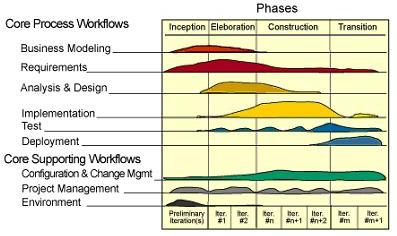
\includegraphics{./imagenes/fasesrup.jpg}
  \caption[\small Fases de RUP y etapas del desarrollo de una aplicaci�n]
  {\small Fases de RUP y etapas del desarrollo de una aplicaci�n \cite{EVE2003}.}
  \label{figfasesrup}
\end{figure}

{\bfseries Iteraciones}\\

Cada fase de RUP puede ser descompuesta en iteraciones. Cada una de estas iteraciones constituye un ciclo completo de la fase, cuyo resultado puede mejorarse siendo sometido a una nueva iteraci�n u otorgar un producto �til para su empleo en la siguiente fase \cite{IBA2003}.\\

Las iteraciones tambi�n pueden ser utilizadas para dividir el sistema en m�dulos, teniendo como objetivo la obtenci�n de un m�dulo completo al final de cada iteraci�n \cite{RAM2001}.\\

{\bfseries Subproductos}\\

Los subproductos (o artefactos como se denominan en RUP) que se obtienen de cada fase son los siguientes \cite{RAM2001}:

\begin{itemize}
\item{\bfseries Fase: Inicio}
	\begin{enumerate}
	\item Alcance del Sistema
	\item	Arquitectura inicial
	\item	Lista inicial de riesgos
	\item	Entorno de desarrollo configurado
	\item	Plan inicial del proyecto
	\item	Caso inicial del negocio
	\end{enumerate}
\item {\bfseries Fase: Elaboraci�n}	
	\begin{enumerate}
	\item Contexto del sistema
	\item Captura del 80\% de los requerimientos funcionales
	\item Arquitectura de referencia
	\item Lista de riesgos
	\item Entorno de desarrollo adecuado
	\item Caso del negocio completo
	\end{enumerate}
\item {\bfseries Fase: Construcci�n}	
	\begin{enumerate}
	\item Modelos completos
	\item Arquitectura �ntegra
	\item Riesgos mitigados
	\item Manual inicial del usuario
	\item Prototipo operacional (beta)
	\item Caso del negocio actualizado
	\end{enumerate}
\item {\bfseries Fase: Transici�n}
	\begin{enumerate}
	\item Prototipo operacional
	\item Documentos legales
	\item Descripci�n de la arquitectura completa y corregida
	\item Manuales
	\end{enumerate}
\end{itemize}



\chapter{AN�LISIS}

Como resultado de esta fase se pretende obtener los requerimientos tanto funcionales como no funcionales (recursos) con los que deber� contar la herramienta propuesta, para que a partir de �stos se pueda proceder al dise�o e implementaci�n.

\section{Definici�n del problema}

El control de la calidad del software no es una tarea f�cil, se requiere de herramientas que ayuden a los expertos en su labor. Por eso, se plantea resolver una parte del problema desarrollando una herramienta de apoyo al control de la calidad del software.\\

El sistema debe ser capaz de ayudar a una empresa en:
\begin{itemize}
\item La coordinaci�n de grupos de trabajo.
\item La distinci�n de usuarios seg�n su grupo (rol).
\item La delegaci�n de responsabilidades a los distintos grupos.
\item El manejo de pruebas (herramientas del SQA) y resultados.
\item El control de asignaci�n de tareas.
\item El mecanismo de alertas.
\item El control de pruebas iterativas sobre un mismo trozo de la aplicaci�n (fases del proyecto, m�dulos del proyecto, fases de los m�dulos � trozos de c�digo).
\item La definici�n del nivel de detalle en las pruebas.
\item La atenci�n de aportes/observaciones del cliente.
\end{itemize}

\section{Tabla de riesgos}

Este apartado se�ala todos los posibles riesgos a los que el proyecto est� sujeto, indicando el tipo de riesgo, la magnitud y el plan de contingencia. La magnitud puede tomar un valor de 1 a 10 dependiendo del grado del problema.

\setlength{\arrayrulewidth}{1pt}
\setlength{\doublerulesep}{0mm}

\begin{longtable}{|c|p{2in}|p{2in}|}
\hline\hline
{Magnitud} & {Descripci�n} & {Estrategia de mitigaci�n / Plan de contingencia}\\ 
\hline		
\footnotesize 9 &	\footnotesize Desarrollo no finalizado a tiempo.	&	\footnotesize Realizar cambios que reduzcan la cantidad de trabajo por realizar.\\
\footnotesize 6	& \footnotesize Problemas con el uso de la tecnolog�a. &	\footnotesize Recurrir a libros y/o  sitios de Internet.\\ 
\footnotesize 5	& \footnotesize Falla a nivel de S.O. o DBMS al implantar la herramienta.	& \footnotesize Realizar pruebas durante la implementaci�n en el S.O. y el DBMS.\\
\hline\hline
\caption{Tabla de riesgos} 
\end{longtable} 

\section{Usuarios del sistema}

Se distinguen cinco tipos de usuarios:
\begin{itemize}
\item	Usuario Administrador: que tendr� la capacidad de gestionar las entidades m�s importantes del sistema como proyectos, usuarios y clientes.
\item	Usuario L�der de proyectos: es el usuario que ser� responsable del control y supervisi�n del avance de los proyectos que tenga a su cargo.
\item	Usuario Tester: es el usuario encargado del control de calidad como tal. Es quien podr� ejecutar los casos de prueba y listas de control y reportar los resultados.
\item	Usuario Desarrollador: que recibir� del tester el reporte del resultado del control de calidad y ser� responsable de la correcci�n de los defectos que el tester le comunique mediante la herramienta.
\item	Usuario Cliente: es el due�o del sistema, quien podr� -en las aquellas fases que el administrador y l�der de proyectos le permitan- aportar sus observaciones a medida que el sistema es desarrollado.
\end{itemize}

\section{Requerimientos}

\subsection{Requerimientos funcionales}

Los requerimientos funcionales definen todas las tareas que el sistema debe ser capaz de hacer (pero no c�mo las har�, para ello est� el dise�o). La definici�n de estos requerimientos es fundamental para el desarrollo del sistema ya que establecer� los l�mites de aquello que queda dentro y fuera del producto.\\

La herramienta del UML que permite la identificaci�n de los requerimientos funcionales de manera sencilla son los diagramas de casos de uso.\\

De los diagramas presentados en las figuras \ref{figusuariogeneral}-\ref{figactorsistema} (y de su detalle expuesto en el Anexo \ref{anexodiagramasyfunciones}), se rescatan los siguientes requerimientos funcionales de acuerdo al tipo de usuario: \\

{\bfseries Actor general}\\

El siguiente diagrama se aplica a administradores, l�deres de proyectos, testers y desarrolladores.\\
 
\begin{figure}[!ht]
  \centering
  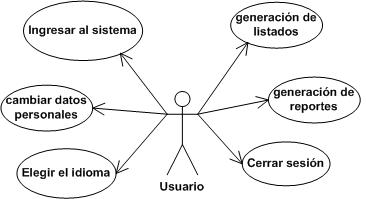
\includegraphics{./imagenes/usuariogeneral.jpg}
  \caption[\small Diagrama de casos de uso para un usuario gen�rico de la herramienta]
  {\small Diagrama de casos de uso para un usuario gen�rico de la herramienta.}
  \label{figusuariogeneral}
\end{figure}

\begin{itemize}
\item	Ingreso al sistema, incluyendo la validaci�n de los datos que el usuario ingrese. 
\item	Elecci�n del idioma con el que desea trabajar.
\item	Modificaci�n sus datos personales (como la contrase�a). A manera de ejemplo, la figura \ref{figusuariogeneral2} muestra este caso de uso detallado.
\item	Generaci�n de listas de datos.
\item Generaci�n de reportes estad�sticos que estar�n disponibles seg�n el rol del usuario.
\item	Cerrar la sesi�n que inici� al ingresar al sistema.
\end{itemize}
 
\begin{figure}[!ht]
  \centering
  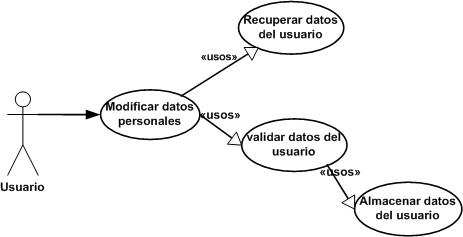
\includegraphics{./imagenes/usuariogeneral2.jpg}
  \caption[\small Caso de Uso: Modificar datos personales]
  {\small Caso de Uso: Modificar datos personales.}
  \label{figusuariogeneral2}
\end{figure}
 
{\bfseries Actor administrador}

\begin{figure}[!ht]
  \centering
  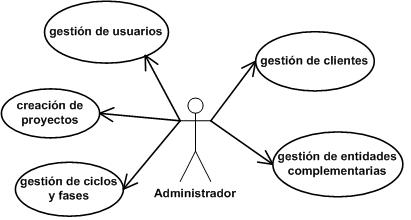
\includegraphics{./imagenes/actoradministrador.jpg}
  \caption[\small Diagrama general de casos de uso para un usuario de tipo Administrador]
  {\small Diagrama general de casos de uso para un usuario de tipo Administrador.}
  \label{figactoradministrador}
\end{figure}
 
\begin{itemize}
\item	Gesti�n de usuarios: creaci�n, incluyendo la asignaci�n de un tipo (administrador, l�der de proyectos, tester, desarrollador o cliente), modificaci�n de datos, habilitaci�n, bloqueo y eliminaci�n de cuentas.
\item	Creaci�n de proyectos lo que incluye la elecci�n del ciclo de vida y asignaci�n de: l�der del proyecto, responsable del control de calidad y responsable del desarrollo.
\item	Gesti�n de clientes.
\item	Administraci�n de ciclos de vida y fases.
\item	Gesti�n de las entidades secundarias como estados, prioridades, niveles, entornos, etc.
\end{itemize}

{\bfseries Actor l�der de proyectos}

\begin{figure}[!ht]
  \centering
  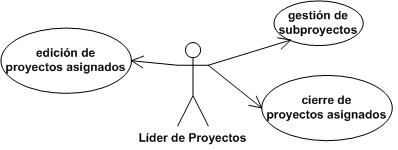
\includegraphics{./imagenes/actorlider.jpg}
  \caption[\small Diagrama general de casos de uso para un usuario de tipo L�der de Proyecto.]
  {\small Diagrama general de casos de uso para un usuario de tipo L�der de Proyecto.}
  \label{figactorlider}
\end{figure}

\begin{itemize}
\item	Gesti�n de subproyectos, lo que incluye la asignaci�n de responsable de control de calidad y desarrollo para cada uno.
\item	Edici�n de datos de los proyectos que tiene asignados.
\item	Cierre de los subproyectos y proyectos del que es responsable.
\end{itemize}

{\bfseries Actor tester}

\begin{figure}[!ht]
  \centering
  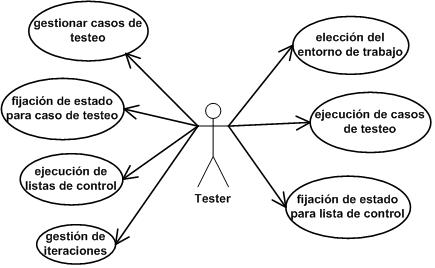
\includegraphics{./imagenes/actortester.jpg}
  \caption[\small Diagrama general de casos de uso para un usuario de tipo Tester]
  {\small Diagrama general de casos de uso para un usuario de tipo Tester.}
  \label{figactortester}
\end{figure}
 
\begin{itemize}
	\item Gesti�n de Casos de Prueba (creaci�n, modificaci�n y eliminaci�n).
	\item Gesti�n de Listas de Control (creaci�n, modificaci�n y eliminaci�n).
	\item Gesti�n de Iteraciones, que incluye la asignaci�n de Casos de Prueba y Listas de Control durante su creaci�n, as� como tambi�n la adici�n y retiro de �stas herramientas durante la ejecuci�n de las iteraciones.	
	\item	Ejecuci�n de los Casos de Prueba (C.P.) y Listas de Control (L.C.) en las iteraciones.
	\item	Elecci�n de un estado resultante de la ejecuci�n de cada C.P. y cada L.C. en las iteraciones.
	\item Asignaci�n de tareas a desarrolladores cuando la ejecuci�n de C.P. y L.C. en las iteraciones terminen con resultados negativos.
	\item	Elecci�n del entorno de trabajo para la ejecuci�n de iteraciones (entorno de hardware y software, versi�n del sistema, etc.).
\end{itemize}

{\bfseries Actor desarrollador}

\begin{figure}[!ht]
  \centering
  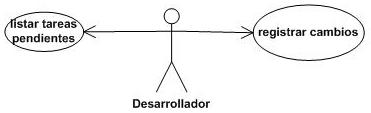
\includegraphics{./imagenes/actordesarrollador.jpg}
  \caption[\small Diagrama general de casos de uso para un usuario Desarrollador]
  {\small Diagrama general de casos de uso para un usuario Desarrollador.}
  \label{figactordesarrollador}
\end{figure}
 
\begin{itemize}
\item	Generaci�n de reportes en caso de que el usuario sea responsable del desarrollo de un subproyecto.
\item	Listado de las tareas pendientes relacionadas a C.P. y L.C. que dieron resultados negativos al finalizar su ejecuci�n en las iteraciones.
\item	Consulta del detalle de cada uno de los casos de prueba asignados.
\item	Cambio de estado de los casos de prueba y listas asignados.
\end{itemize}

{\bfseries Actor cliente}

\begin{figure}[!ht]
  \centering
  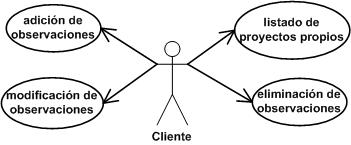
\includegraphics{./imagenes/actorcliente.jpg}
  \caption[\small Diagrama general de casos de uso para un usuario Cliente]
  {\small Diagrama general de Casos de Uso para un usuario Cliente.}
  \label{figactorcliente}
\end{figure}
 
\begin{itemize}
\item	Acceso a los proyectos de los que es due�o.
\item	Adici�n, modificaci�n y eliminaci�n de observaciones sobre una determinada fase de un subproyecto de un proyecto en particular.
\item	Listado de las observaciones expuestas previamente.
\end{itemize}

{\bfseries Actor sistema}\\

A los cinco tipos de usuarios se�alados previamente, se a�ade un sexto que es el Sistema, al cual se le atribuyen funciones que deber� efectuar autom�ticamente.

\begin{figure}[!ht]
  \centering
  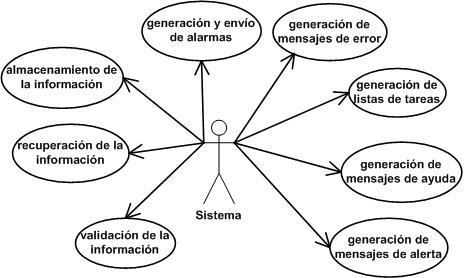
\includegraphics{./imagenes/actorsistema.jpg}
  \caption[\small Diagrama de casos de uso para la herramienta]
  {\small Diagrama de casos de uso para la herramienta.}
  \label{figactorsistema}
\end{figure} 

\begin{itemize}
\item	Generaci�n de alarmas para l�deres de proyectos, testers y desarrolladores sobre las tareas pendientes que tiene cada uno.
\item Generaci�n de alarmas para l�deres de proyectos y administradores cuando los subproyectos y proyectos pueden cerrarse.
\item	Generaci�n de listas sobre las tareas pendientes de cada usuario.
\item	Env�o de alertas mediante distintos medios como el correo electr�nico.
\item	Generaci�n de mensajes al usuario en los casos en que una fase, un subproyecto o un proyecto est�n en condiciones de ser cerrados.
\item	Control de errores durante el registro de los datos (controlando la integridad de los datos y la coherencia entre ellos).
\item	Recuperaci�n de la informaci�n cuando se requiera (acceso a la Base de Datos y ejecuci�n de las consultas necesarias seg�n la solicitud del Controlador de cada entidad).
\item	Almacenamiento de la informaci�n cuando se le solicite (actualizaciones a las tablas de la Base de Datos como respuesta a solicitudes del Controlador de cada entidad).
\end{itemize}

\subsection{Requerimientos no funcionales}

Los requerimientos no funcionales definen b�sicamente las propiedades del sistema, sus restricciones y los factores externos al producto. Las propiedades del sistema pueden ser, por ejemplo, requerimientos impl�citos que debe cumplir como la confiabilidad y la exactitud. Las restricciones son las capacidades de los recursos que el sistema utilizar�, como la memoria, procesador, etc. \cite{SOM1996}.\\
 
{\bfseries Requerimientos no funcionales del producto}
\begin{itemize}
\item La herramienta debe contar con una documentaci�n apropiada.
\item Requerimientos impl�citos (seguridad, robustez, exactitud, etc.).
\item La herramienta debe ser f�cil de usar y contar con manuales (ver secci�n \ref{seccionmanuales}) para cada tipo de usuario.
\end{itemize}

{\bfseries Restricciones}
\begin{itemize}
\item El sistema deber� ejecutarse en un servidor que tenga los siguientes requerimientos:
	\begin{itemize}
	\item Sistema Operativo: Windows 98 o Linux 7.0
	\item Servidor Web: Apache 1.3 con la distribuci�n de PHP 3.0 incluida, porque existen funciones del lenguaje utilizadas en la aplicaci�n que exigen estas versiones de Apache y PHP como m�nimo.
	\item Servidor de SMTP instalado para el env�o de alertas.
	\item Memoria RAM de 128 MB.
	\item Procesador de 500 Mhz como m�nimo. Se debe tomar en cuenta que el servidor atender� a m�s de un usuario a la vez y mientras m�s lento sea el procesador, mayor ser� el tiempo de respuesta a cada solicitud. Tambi�n hay que recordar que la aplicaci�n est� escrita en PHP y por lo tanto todo el procesamiento se hace del lado del servidor. 
	\item Espacio libre m�nimo en disco duro: 59 MB para:
			\begin{itemize}
			\item Almacenamiento del c�digo fuente de la aplicaci�n: 10 MB.
			\item Almacenamiento de la Base de Datos en caso de que �sta resida en el servidor y se utilice MySQL como DBMS: 10 MB.
			\item 200 KB de espacio por archivo que sea subido al servidor desde un cliente. Un promedio de 10 archivos por proyecto, y un n�mero aproximado de 20 proyectos hacen un total de 39 MB para el almacenamiento de documentos de los proyectos.
			\end{itemize}
	\end{itemize}
	
\item Cada cliente que se conecte al servidor para hacer uso de la herramienta deber� contar con un m�nimo de:
	\begin{itemize}
	\item	Sistema Operativo: Windows 98 o Linux 7.0.
	\item	Navegador: Internet Explorer 5.0 (si el S.O. es Windows) o Netscape 6.0.
	\item	Memoria RAM: 64 MB.
	\item	Procesador: 333 Mhz.
	\item	Espacio en Disco Duro: opcional seg�n la cantidad de documentos que el usuario desee descargar de la aplicaci�n.
	\item	Tarjeta de Red 10/100 o bien, una conexi�n a Internet con una velocidad m�nima de transferencia de 50 Kbps (dependiendo del tipo de acceso que el cliente tenga al servidor).
	\item	Impresora en caso de desear tener los reportes impresos en papel.
	\end{itemize}
\end{itemize}

\section{Diagramas de colaboraci�n} \label{diagramacolaboracion}

Estos diagramas muestran de manera gr�fica las interacciones que existen alrededor de los roles. Permiten identificar mediante los denominados clasificadores las potenciales clases del sistema \cite{RUM2000}.\\

A manera de ejemplo, se presenta el diagrama de la figura \ref{figcolaboracioncrearcaso}, que muestra las distintas interacciones (numeradas por orden de la secuencia que se sigue) que existir�n entre el usuario, el sistema (en el esquema se presenta a �ste desglosado en las tres capas del modelo MVC) y el repositorio de datos. Los clasificadores son:
\begin{itemize}
\item La Vista
\item El controlador
\item El validador
\item El Caso de Testeo
\item Base de Datos
\end{itemize}

\begin{figure}[!ht]
  \centering
  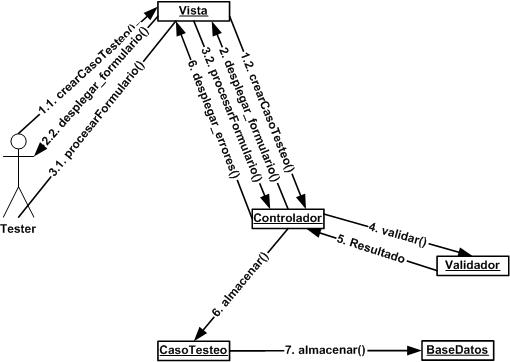
\includegraphics{./imagenes/colaboracioncrearcaso.jpg}
  \caption[\small Diagrama de colaboraci�n: crear un caso de testeo]
  {\small Diagrama de colaboraci�n: crear un caso de testeo.}
  \label{figcolaboracioncrearcaso}
\end{figure} 
 
Estos clasificadores son comunes a casi todas las funciones de la aplicaci�n, a excepci�n del cuarto que es reemplazado por las entidades que se vean involucradas en cada funci�n.

\section{Diagrama de estados} \label{diagramaestados}

Muestra los distintos estados por los que pasa un objeto durante la ejecuci�n de una funci�n \cite{RUM2000}. El diagrama que se muestra en la figura \ref{figestados} muestra todo el proceso que se sigue desde que el usuario entra al sistema y elige el proyecto hasta que lo cierra y termina su sesi�n en la aplicaci�n.\\

La secuencia que es descrita en el diagrama est� explicada ``en modo texto'' en el algoritmo de la secci�n \ref{seccionalgoritmos} (Algoritmos).\\
 
\begin{figure}[!ht]
  \centering
  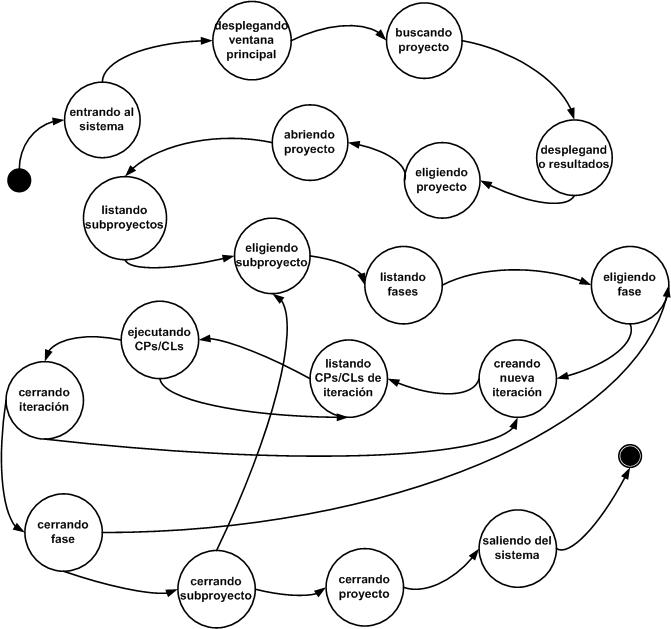
\includegraphics[width=\textwidth]{./imagenes/estados.jpg}
  \caption[\small Diagrama de estados que ilustra el proceso de control de calidad de un proyecto]
  {\small Diagrama de estados que ilustra el proceso de control de calidad de un proyecto.}
  \label{figestados}
\end{figure} 

Hasta aqu� se hizo el an�lisis de la herramienta, extrayendo los requerimientos y una visi�n global de la l�gica que �sta debe seguir.



\chapter{DISE�O}

Al finalizar esta etapa del desarrollo se cuenta con los diagramas completos de casos de uso, secuencia, estados, clases y otros complementarios, que den paso finalmente a la fase de implementaci�n.

\section{Diagramas de secuencia}
 
Como continuaci�n a los diagramas de colaboraci�n y estado obtenidos del an�lisis es necesario crear los diagramas de secuencia. �stos muestran las interacciones entre los distintos objetos organizadas en una secuencia temporal, lo que los hace ser en este aspecto diagramas m�s elaborados que los de Colaboraci�n \cite{RUM2000}. Las interacciones son denominadas mensajes.\\

Los diagramas de secuencia constituyen un puente entre los diagramas de colaboraci�n (donde se presentan los clasificadores o potenciales clases) y el diagrama de clases que ser� mostrado en la secci�n \ref{disenio}.\\

El diagrama mostrado en la figura \ref{figdiagramasecuencia1} corresponde a la funci�n ``Ingresar al sistema''.

\begin{figure}[!ht]
  \centering
  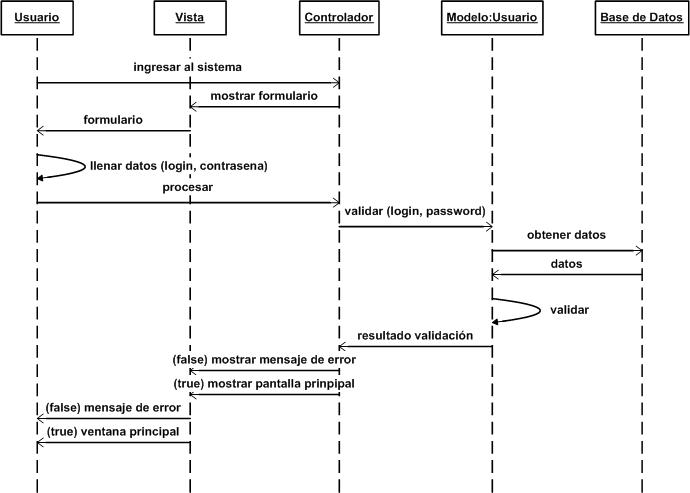
\includegraphics[width=13cm]{./imagenes/secuenciaingresarsistema.jpg}
  \caption[\small Diagrama de secuencia para la funci�n Ingresar al Sistema]
  {\small Diagrama de secuencia para la funci�n Ingresar al Sistema.}
  \label{figdiagramasecuencia1}
\end{figure}

En el diagrama se presentan los clasificadores mencionados en la secci�n \ref{diagramacolaboracion} (Diagrama de colaboraci�n).\\

La figura tambi�n describe la manera en que trabajan las capas del modelo MVC: Toda solicitud llega primero al Controlador mediante la Vista. Seg�n el tipo de requerimiento, �ste (Controller) solicita datos del Modelo. Los resultados de este �ltimo definen el tipo de respuesta que el Controlador ordenar� a la Vista desplegar.\\

En el Anexo \ref{anexodiagramasyfunciones} se encuentran los diagramas de casos de uso, colaboraci�n, estado y secuencia de las funciones del sistema seg�n el tipo de usuario.

\section{Clases} \label{disenio}

El diagrama presenta las clases involucradas en el sistema en t�rminos de estructura y de herencia. Como es de esperarse, la definici�n de toda clase trae consigo la definici�n de sus atributos y m�todos, lo que aporta mucha informaci�n a los dise�adores para proceder a la elaboraci�n de modelos como el presentado en el siguiente apartado (\ref{secentidadrelacion} Diagrama entidad-relaci�n) y de algoritmos \cite{RUM2000}.\\

La figura \ref{figdiagramaclases} muestra las distintas clases involucradas en el sistema y las relaciones entre ellas. Las clases carecen de atributos y m�todos en el gr�fico con el objetivo de facilitar su visualizaci�n; el detalle de cada clase se encuentra en el Anexo \ref{anexodiccionarioclases} (Diccionario de Clases).\\

\begin{figure}[!ht]
  \centering
  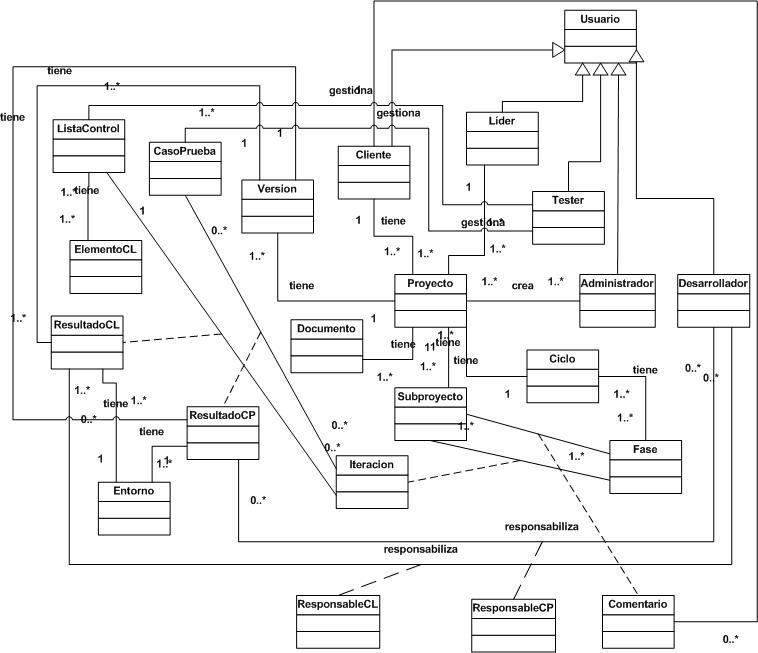
\includegraphics[width=13cm]{./imagenes/diagramaclases.jpg}
  \caption[\small Diagrama de clases]
  {\small Diagrama de clases.}
  \label{figdiagramaclases}
\end{figure}

En base a �ste diagrama y al de estados mostrado en la secci�n \ref{diagramaestados} se obtuvo el algoritmo mostrado en el apartado \ref{seccionalgoritmos}.

\section{Diagrama entidad-relaci�n}
\label{secentidadrelacion}

Este modelo fue obtenido en base al Modelo de Clases con el objetivo de obtener un modelo relacional para la creaci�n de la Base de Datos.\\

{\bfseries{Del diagrama de clases al diagrama E-R}}\\

Para hacer la conversi�n se utilizaron los siguientes criterios (sugeridos por \cite{RUM1996}):
\begin{itemize}
\item	Cada clase se convierte en una o m�s tablas.
\item	Cada atributo de una clase se convierte en una columna de la tabla que corresponder� a la entidad. A esto se a�aden uno o m�s campos (o se identifican de los ya existentes) que conformen la clave principal.
\item	De relaciones m�ltiples (n:n) surgen tablas intermedias como resultado de la normalizaci�n.
\end{itemize}

La figura \ref{figdiagramaer} muestra el diagrama E-R de la aplicaci�n. A pesar de que se obtuvo el modelo de Base de Datos relacional con este diagrama, las clases no desaparecen del Dise�o de la aplicaci�n puesto que ser�n utilizadas posteriormente durante la implementaci�n de la Capa M del modelo MVC (v�ase el cap�tulo \ref{capimplementacion}: Implementaci�n).\\

\begin{figure}[!ht]
  \centering
  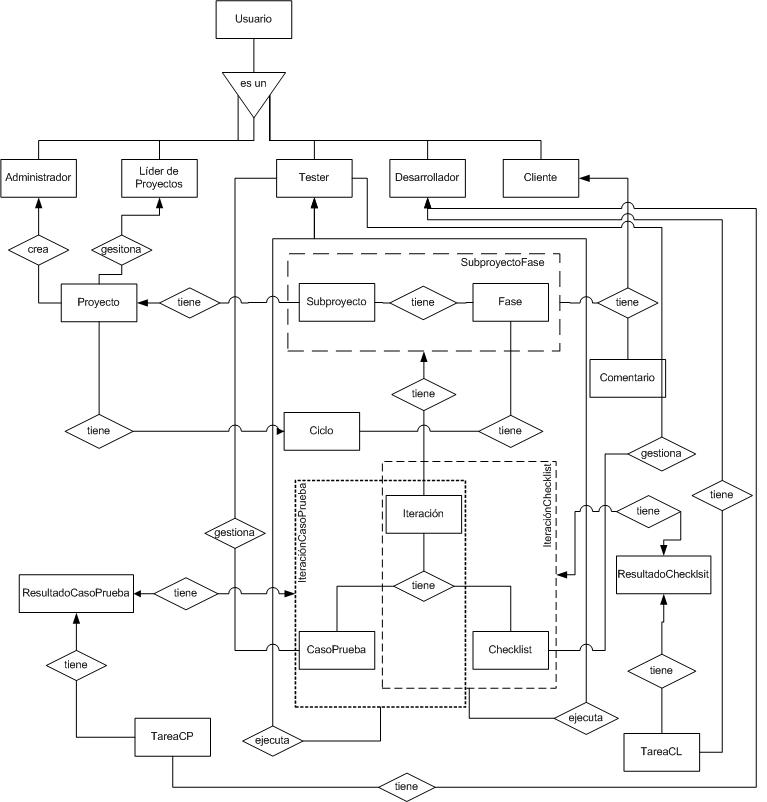
\includegraphics[width=15cm]{./imagenes/modeloer2.jpg}
  \caption[\small Diagrama entidad-relaci�n]
  {\small Diagrama entidad-relaci�n.}
  \label{figdiagramaer}
\end{figure}
 
El Diccionario de Datos que acompa�a al diagrama presentado se encuentra detallado en el Anexo \ref{anexodiccionariodatos}.

\clearpage
\section{Algoritmo} \label{seccionalgoritmos}

El algoritmo presentados a continuaci�n es una contribuci�n personal al dise�o del sistema.\\

{\bfseries Controlar la calidad de un proyecto}\\

El siguiente algoritmo muestra la manera en que los usuarios pueden efectuar el control de la calidad de un proyecto (en general). El algoritmo muestra toda la l�gica de la aplicaci�n en torno a un objeto de la clase Proyecto. En esta l�gica intervienen los usuarios y el sistema.

\begin{figure}[!ht]
  \centering
  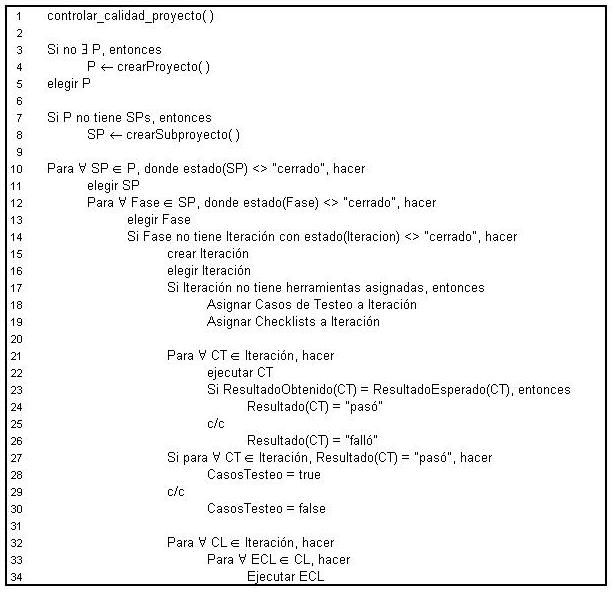
\includegraphics[width=15cm]{./imagenes/algoritmo_1.jpg}  
  \label{figalgoritmo1}
\end{figure}

\clearpage
\begin{figure}[!ht]
  \centering
  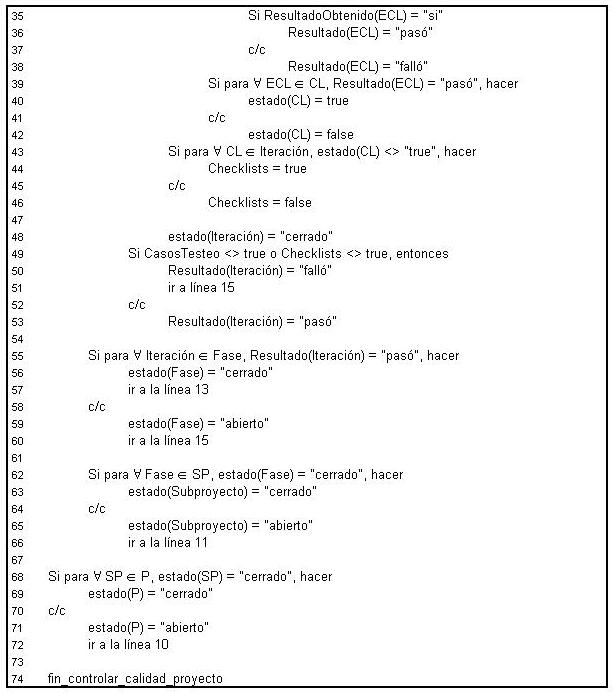
\includegraphics[width=15cm]{./imagenes/algoritmo_2.jpg}  
  \label{figalgoritmo2}
\end{figure}


\section{Arquitectura}

La arquitectura del sistema define la organizaci�n f�sica y l�gica que tendr� la aplicaci�n.

\subsection{Organizaci�n f�sica}

Esta organizaci�n se divide en dos: la organizaci�n general de la aplicaci�n y la organizaci�n espec�fica que �sta tendr� en el servidor.\\

\clearpage
{\bfseries a. Enfoque general}\\

La figura que se muestra a continuaci�n muestra un esquema de las tres capas que tendr� la aplicaci�n (Cliente, Servidor y Base(s) de Datos).\\

\begin{figure}[!ht]
  \centering
  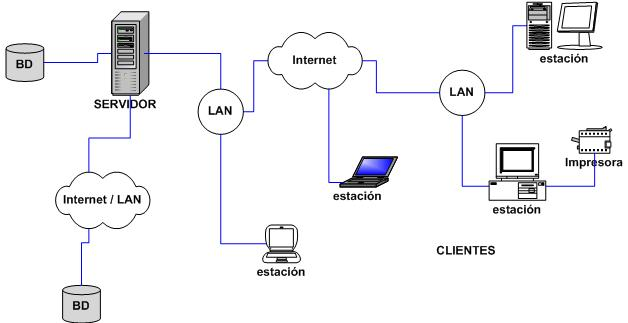
\includegraphics{./imagenes/arquitecturageneral.jpg}
  \caption[\small Arquitectura general de la aplicaci�n (three-tier)]
  {\small Arquitectura general de la aplicaci�n (three-tier).}
  \label{figarquitecturageneral}
\end{figure}  

Como se ve en la figura, un cliente podr� acceder al servidor mediante una LAN  (o cualquiera de las variantes conocidas de redes como MAN  y WAN ), directamente por Internet � ambos (LAN y luego Internet). A su vez, del lado del servidor, se tendr� un esquema similar: el acceso al mismo podr� ser directo desde Internet o pasando por �ste y luego por una subred.\\

De una manera an�loga, la Base de Datos podr� residir en el mismo servidor o bien, en otra m�quina, siendo accedida mediante una red (LAN, MAN, WAN o Internet). De todas formas, la arquitectura continuar� siendo de tres capas.\\

{\bfseries b. Componentes}\\

Un diagrama de componentes es utilizado para modelar la estructura del software incluyendo las dependencias entre los distintos componentes.\\

El diagrama de la figura \ref{figcomponentes} muestra los componentes de la aplicaci�n y la relaci�n de dependencia (flecha con trazo discontinuo) que existe entre ellos.\\

B�sicamente, un componente se define como una parte f�sica del sistema que contiene parte de la implementaci�n del mismo. Puede o no depender de otros componentes y ser reemplazado si es necesario por uno o m�s nuevos. Contiene c�digo fuente y su estructura interna y contenido puede responder a las convenciones del lenguaje de programaci�n utilizado \cite{RUM2000}.

\begin{figure}[!ht]
  \centering
  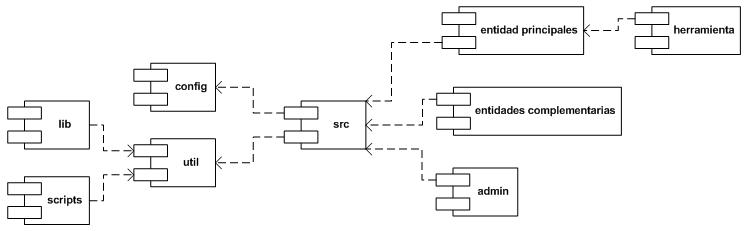
\includegraphics[width=\textwidth]{./imagenes/componentes2.jpg}
  \caption[\small Diagrama general de componentes]
  {\small Diagrama general de componentes.}
  \label{figcomponentes}
\end{figure}

\begin{itemize}
\item	Config.- contiene archivos de configuraci�n del sistema
\item	Util.- contiene librer�as y archivos complementarios que ser�n comunes a m�s de un objeto del sistema. 
\item	Src.- Depende de los dos anteriores y contiene todo el c�digo fuente de la aplicaci�n, organizado por entidades.
\end{itemize}

Como complemento al diagrama de la figura \ref{figcomponentes}, se presenta la figura \ref{figarquitecturaservidor} que detalla la organizaci�n de la aplicaci�n a nivel f�sico dentro del servidor.
 
\begin{figure}[!ht]
  \centering
  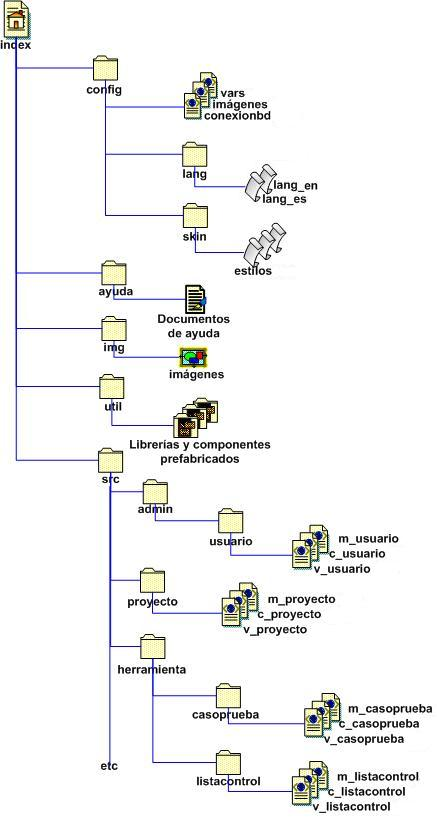
\includegraphics{./imagenes/arquitecturaservidor.jpg}
  \caption[\small Organizaci�n f�sica de la aplicaci�n dentro del servidor]
  {\small Organizaci�n f�sica de la aplicaci�n dentro del servidor.}
  \label{figarquitecturaservidor}
\end{figure}

\clearpage

\subsection{Organizaci�n l�gica}

Muestra la manera en que los archivos se organizan para garantizar el correcto funcionamiento de la aplicaci�n y una estructura l�gica coherente y ordenada.\\

Esta organizaci�n est� basada en la propuesta por la arquitectura MVC, que como se explic� en el cap�tulo 4, ser� utilizada para la implementaci�n de la herramienta.\\

{\bfseries a. Paquetes}\\

Un paquete es una parte un modelo. Cada paquete contiene un conjunto de partes m�s peque�as del modelo, asignadas bajo un mismo principio (como la funcionalidad) \cite{RUM2000}.\\

En la figura \ref{figpaquetes} se muestra el diagrama de paquetes de la aplicaci�n y las clases m�s importantes que cada paquete contendr�.\\

\begin{figure}[!ht]
  \centering
  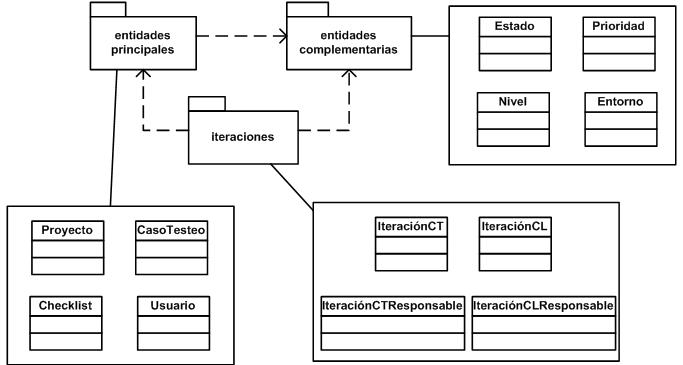
\includegraphics[width=15cm]{./imagenes/paquetes.jpg}
  \caption[\small Diagrama de paquetes]
  {\small Diagrama de paquetes.}
  \label{figpaquetes}
\end{figure} 

\clearpage
{\bfseries b. Capas MVC}\\

La figura \ref{figorganizacionlogica} ilustra la disposici�n de las capas del modelo MVC en la organizaci�n l�gica de la aplicaci�n. Como ejemplo, se muestra el caso de la entidad Proyecto que:
\begin{itemize}
\item En la capa de la Vista podr� tener archivos para listar los proyectos, crear nuevos, editar los existentes, eliminar, etc.
\item En la capa del Controlador tendr� dos archivos: uno ``maestro'' que se ocupar� de invocar a todos los archivos del Modelo que necesite (es por eso que en el ejemplo aparecen en la capa del Modelo las entidades proyecto, cliente, usuario y ciclo) y otro que servir� de soporte al primero durante la validaci�n de la informaci�n.
\end{itemize}

\begin{figure}[!ht]
  \centering
  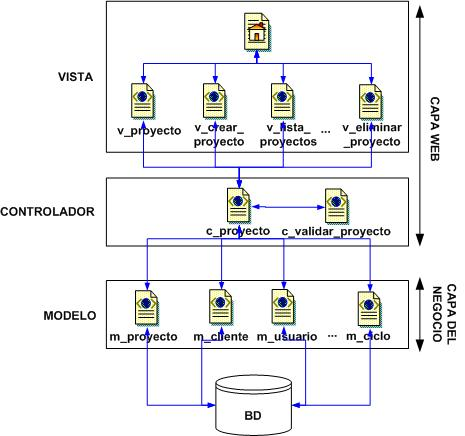
\includegraphics{./imagenes/arquitecturalogica.jpg}
  \caption[\small Organizaci�n l�gica de la aplicaci�n]
  {\small Organizaci�n l�gica de la aplicaci�n. En la figura se muestra como ejemplo la organizaci�n de archivos para la entidad Proyecto.}
  \label{figorganizacionlogica}
\end{figure}  

\chapter{IMPLEMENTACI�N}
\label{capimplementacion}

En este cap�tulo se detallan los aspectos concernientes a la codificaci�n de la herramienta y otros que tienen como objetivo alcanzar una versi�n operable del producto.

\section{Elecci�n de las herramientas de implementaci�n}

Para la implementaci�n de la Herramienta Web de apoyo al control de la calidad del software, se decidi� utilizar las siguientes herramientas:
\begin{itemize}
\item	Lenguaje de programaci�n: Hipertext PreProcessor (PHP).
\item	Servidor: Apache. 
\item	Servidor de Base de Datos: MySQL.
\end{itemize}

{\bfseries PHP}\\

PHP\footnote{www.php.net}  es el acr�nimo de Hypertext Preprocessor. Es un lenguaje ``open source''\footnote{Open source: C�digo abierto, gratuito.} interpretado de alto nivel que es escrito en p�ginas HTML y ejecutado del lado del servidor.\\\\
La figura \ref{figejecucionphp} muestra la manera en que se ejecutan las aplicaciones escritas en PHP.\\

\begin{figure}[!ht]
  \centering
  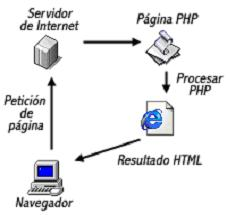
\includegraphics{./imagenes/ejecucionphp.jpg}
  \caption[\small Ejecuci�n de un programa escrito en PHP]
  {\small Ejecuci�n de un programa escrito en PHP \cite{WEB2003}.}
  \label{figejecucionphp}
\end{figure} 

{\bfseries Ventajas \cite{IGN2003}\cite{ASC2003}\cite{PHP2004}}\\
\begin{enumerate}
\item	Al heredar las caracter�sticas (sintaxis por ejemplo) de lenguajes tradicionales como C/C++, es sencillo de aprender para programadores que han tenido un m�nimo de experiencia con tales lenguajes.
\item	Ofrece un conjunto bastante amplio y completo de funciones que simplifican el trabajo del desarrollador. Estas funciones ofrecen la posibilidad de manejar clases, bases de datos, archivos, cadenas, etc.
\item	Cuenta con bastante documentaci�n, fruto del trabajo de sus creadores, profesionales y aficionados que han puesto a disposici�n de los interesados los resultados de sus investigaciones, experiencias y trabajos.
\item	Es multiplataforma, lo que permite que las aplicaciones escritas en este lenguaje sean independientes del Sistema Operativo y del Servidor.
\item	Al ser un lenguaje interpretado, reduce el tiempo de desarrollo al permitir la ejecuci�n inmediata del c�digo sin previas compilaciones. Adem�s resulta m�s ligero para el servidor y su ejecuci�n es mucho m�s r�pida.
\item	Es robusto. Su sistema de control de errores es bastante bueno y detallado al momento de detectar y reportar fallas en el c�digo.
\item	Soporta (de manera b�sica) el paradigma de programaci�n Orientada a Objetos.
\item	El an�lisis l�xico para el reconocimiento de variables que se pasan en la direcci�n es autom�tico.
\item	Permite la incrustaci�n de etiquetas HTML en su c�digo.
\item	Su soporte de acceso a Bases de Datos es muy bueno.
\item	No maneja el concepto de punteros como lo hacen otros lenguajes como C/C++, lo que facilita el trabajo al desarrollador, evita problemas de depuraci�n y otros asociados con accesos a memoria.
\item	El c�digo PHP es mucho m�s legible e interpretable que el c�digo de otros lenguajes.
\item	Como se dijo en el p�rrafo introductorio, es un lenguaje ``open source'', es decir, gratuito y de f�cil acceso (esto incluye el acceso a un amplio conjunto de aplicaciones listas para reutilizarse que son ofrecidas por la comunidad que apoya PHP).
\item	Su aceptaci�n por parte de millones de desarrolladores lo han convertido en uno de los lenguajes para desarrollo Web m�s populares y ricos en documentaci�n y recursos. La figura F.2 muestra el r�pido de crecimiento de servidores que utilizan PHP.
\item	Se ejecuta completamente del lado del servidor, con esto se garantiza que la aplicaci�n no dependa de qu� tecnolog�a usa el cliente que acceda a la aplicaci�n. B�sicamente, �ste s�lo requiere de un navegador.
\item	En comparaci�n con otros lenguajes interpretados (como Perl), PHP garantiza una curva de aprendizaje mejor ya que es sencillo de aprender.\\
\end{enumerate}

\begin{figure}[!ht]
  \centering
  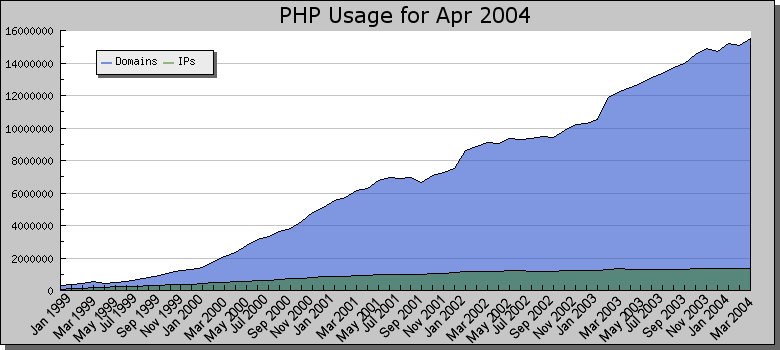
\includegraphics[width=\textwidth]{./imagenes/usophp2.png}
  \caption [\small Gr�fica del n�mero de dominios y direcciones IP que utilizan PHP]
  {\small Gr�fica del n�mero de dominios y direcciones IP que utilizan PHP.
Estad�stica de Netcraft \cite{NET2004}.}
  \label{figusophp}
\end{figure} 
 
{\bfseries Desventajas \cite{ASC2003}}
\begin{enumerate}
\item	No deja ning�n tipo de tarea al cliente. Exige que todo el trabajo sea hecho en el servidor lo que en algunos casos resulta inconveniente debido al retardo que ocasiona en la respuesta de tareas que pueden perfectamente ser hechas del lado del cliente.
\item	El hecho de poder mezclar c�digo PHP con HTML puede resultar perjudicial si no se establece un buen conjunto de convenciones de programaci�n.
\item	La manipulaci�n de Clases y Objetos es muy precaria aun y puede resultar perjudicial para sistemas muy grandes.
\end{enumerate}

Para que estas desventajas no afecten el correcto y eficiente funcionamiento del sistema se establecieron las siguientes convenciones:
\begin{enumerate}
\item	Debido a que se desea que el sistema sea multiplataforma ser� necesario que todas las tareas sean hechas por el Servidor, as� no se depender� del Cliente en absoluto. El costo de esta decisi�n es la velocidad de la aplicaci�n. Sin embargo, debido a que PHP es interpretado y ofrece un excelente manejo de la memoria, se espera que el tiempo de respuesta sea m�nimo.
\item Para no tener c�digo PHP y HTML mezclado en toda la aplicaci�n se decidi� s�lo utilizar �ste �ltimo en la capa View de la arquitectura MVC.
\item En cuanto a las Clases y Objetos, el soporte y manipulaci�n ofrecidos por PHP son suficientes para la aplicaci�n debido a que s�lo se utilizar�n Clases en la capa Model de la arquitectura MVC.
\end{enumerate}

\vspace*{0.3cm}
{\bfseries PHP y otros lenguajes \cite{ORA2004}\cite{PHP2004}}
\vspace*{0.3cm}

\begin{itemize}

\item PHP y ASP/ASP.NET.- Las ventajas que PHP presenta frente a ASP/ASP.NET son las siguientes: 
	\begin{enumerate}
	\item Es de libre distribuci�n.
	\item Es multiplataforma (ASP y ASP.NET requieren de Win32 y el IIS).
	\item Es m�s eficiente en el uso de recursos.
	\item Es m�s seguro.
	\item Cuenta con c�digo de libre distribuci�n.	
	\end{enumerate}

\item PHP y ColdFusion.- Aunque ColdFusion tiene una mejor manipulaci�n de errores y manejo de los datos, PHP corre en muchas m�s plataformas, es mucho m�s eficiente en tareas complejas, brinda una mayor estabilidad, flexibilidad y una mejor manipulaci�n de estructuras anidadas. Adem�s, PHP cuenta con mucha m�s documentaci�n.

\item PHP y Perl.- La gran ventaja de PHP frente a Perl es la curva de aprendizaje. Perl es mucho m�s complicado de aprender. Adem�s, PHP es m�s r�pido en tiempo de ejecuci�n.

\item PHP y Java.- Java fue considerado en un principio como el lenguaje de programaci�n de la herramienta propuesta en el presente trabajo, sin embargo fue descartado porque presenta las siguientes desventajas frente a PHP:
	\begin{itemize}
	\item Para este caso, Java exig�a la utilizaci�n de diversas tecnolog�as como Struts (MVC en Java), JavaBeans, JSP y Servlets. Esto ocasionaba que el c�digo de la aplicaci�n crezca y se complique m�s de lo necesario y con ello �sta fuera m�s lenta. Adem�s, la curva de aprendizaje no ten�a comparaci�n frente a la de PHP. 
	\item La combinaci�n de distintas tecnolog�as de Java (Struts, JSP, Servlets, etc.) obliga el uso de otros lenguajes que hagan las veces de {\it engranaje} como XML, lo que complica a�n m�s el c�digo.
	\item Java es compilado e interpretado, lo que duplica el tiempo de desarrollo y ejecuci�n de una aplicaci�n. Al ser PHP solo interpretado, permite un desarrollo m�s r�pido y la ejecuci�n inmediata sin previas compilaciones.
	\item PHP maneja mejor los recursos que Java (memoria, procesador).		
	\item El c�digo PHP puede ser escrito en cualquier editor de textos (incluso los ofrecidos de manera gratuita con los Sistemas Operativos) y luego ser llevado a un navegador para su ejecuci�n. Si bien Java tambi�n puede ser escrito en un editor de textos, la complejidad de su c�digo, las compilaciones previas y la inminente necesidad de contar con un ambiente de trabajo que organice los archivos y oriente a los desarrolladores (por la gran cantidad de archivos fuente que se van creando y el manejo de m�todos y atributos en cada uno de ellos), obliga a �stos a adquirir herramientas adicionales (como JBuilder), cuyas versiones completas no son de libre distribuci�n.
	\end{itemize}
\end{itemize}

{\bfseries Apache}\\

El  NCSA (National Center for Super Computing Applications) desarroll�, en 1995, uno de los primeros servidores Web pero el proyecto fracas�.\\

Sin embargo, los usuarios comenzaron a crear parches para el servidor y a intercambiarlos, creando un foro para la administraci�n de estos remiendos. Fue as� que naci� el grupo Apache, que sigue funcionando actualmente y se dedica a perfeccionar el servidor.\\

{\bfseries Ventajas}\\

Las principales ventajas de Apache son \cite{AEI2002}:\\
\begin{enumerate}
\item	Fiabilidad: Alrededor del 90\% de los servidores con m�s alta disponibilidad funcionan con Apache.
\item	Gratuito: Apache es completamente gratuito y se distribuye bajo la licencia Apache Software License\footnote{http://www.apache.org/LICENSE.txt}, que permite la modificaci�n del c�digo.
\item Extensibilidad: se pueden a�adir m�dulos para ampliar las ya de por s� amplias capacidades de Apache.
\end{enumerate}

La figura \ref{figusoapache} muestra las estad�sticas que comparan la aceptaci�n de Apache frente a otros servidores Web \cite{NET2004}.

\begin{figure}[!ht]
  \centering
  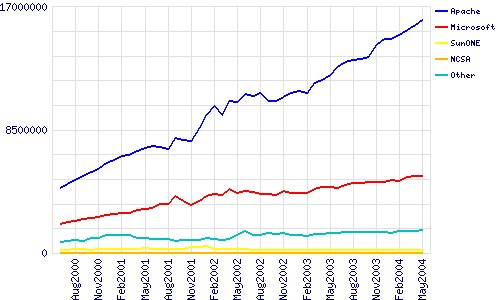
\includegraphics{./imagenes/usoapache2.jpg}
  \caption[\small Servidores Web activos desde agosto de 2000 a mayo de 2004]
  {\small Servidores Web activos desde agosto de 2000 a mayo de 2004 \cite{NET2004}.}
  \label{figusoapache}
\end{figure} 

\clearpage
\section{Marco de trabajo}

El marco de trabajo definido une la arquitectura de desarrollo elegida (MVC) con el lenguaje de programaci�n (PHP).\\

{\bfseries MVC en PHP}\\

Para la implementaci�n de MVC con PHP se determin� utilizar los siguientes recursos del lenguaje en cada capa del modelo:\\
\begin{itemize}
\item Vista: etiquetas HTML, hojas de estilo (css) y estructuras de control b�sicas de PHP (condicionales y ciclos).
\item Controlador: estructuras condicionales para las acciones y redireccionamientos.
\item Modelo: Clases y elementos de conexi�n a Bases de Datos de PHP.
\end{itemize}

Las tres capas est�n acompa�adas de archivos PHP adicionales para la configuraci�n de las variables de entorno, validaciones y otros recursos que deben ser compartidos por las tres capas.\\

La figura \ref{figmvcphp} ilustra el marco de trabajo definido.\\

\begin{figure}[!ht]
  \centering
  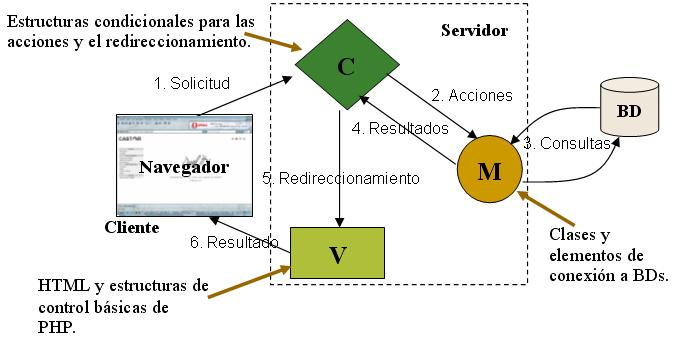
\includegraphics[width=15cm]{./imagenes/mvcphp.jpg}
  \caption[\small Marco de trabajo MVC con PHP]
  {\small Recursos del lenguaje y secuencia de acciones en un 
marco de trabajo MVC con PHP.}
  \label{figmvcphp}
\end{figure} 

Este marco de trabajo fue creado en base al documento de Jacobo Tarr�o: ``MVC en PHP'' \cite{TAR2002}. A esta documentaci�n se hicieron algunos cambios estructurales (como la adici�n de clases y objetos) dando como resultado un framework bastante completo, sencillo de manipular, flexible y robusto.

\section{Hechos relevantes de la implementaci�n}

Como se estableci� en la etapa de dise�o y se explic� en el diagrama expuesto l�neas arriba, la implementaci�n utiliza las siguientes convenciones:
\begin{itemize}
\item	Cada entidad tiene cinco archivos PHP base:
	\begin{itemize}
	\item	Para la Vista: los archivos v\_entidad y v\_entidad\_editar. El primero para desplegar la lista de elementos que esa entidad tiene en la Base de Datos y el segundo para todas las acciones de edici�n (creaci�n, modificaci�n y eliminaci�n).
	\item	Para el Controlador: los archivos c\_entidad y c\_entidad\_validar. El primero que es el encargado de recibir todas las solicitudes de la Vista, instanciar objetos de la capa del Modelo y redireccionar los resultados a nuevos archivos de la Vista. El segundo sirve de soporte al primero en las tareas de validaci�n de datos (las funciones comunes de validaci�n son reutilizadas por todos los archivos c\_entidad\_validar al compartir el archivo general ``validador'' del directorio ``util'').
	\item	Para el modelo: el archivo m\_entidad que contiene una clase con el nombre la entidad que maneja y es el encargado de todos los accesos a la Base de Datos que conciernan a esta.
	\end{itemize}
\item	Se posee adem�s, un conjunto de archivos de configuraci�n entre los que se destacan:
	\begin{itemize}
	\item	ConexionBD: archivo exclusivo para la conexi�n a la Base de Datos. Este script extrae los valores para la conexi�n (nombre de la Base de Datos y cuenta con la cual conectarse) del archivo ``vars''.
	\item	Vars: para la declaraci�n y asignaci�n de valores de las variables de entorno (variables que son compartidas por la mayor�a de los archivos de la aplicaci�n).
	\item	Mensaje: para la configuraci�n de los mensajes de informaci�n, error y advertencia. Este archivo siempre recibe los datos a desplegar del archivo controlador que lo invoca cuando es necesario mostrar un mensaje al usuario.
	\end{itemize}
\end{itemize}

\section{La aplicaci�n}

El nombre asignado a la herramienta es CASTOR.\\

\subsection{Descripci�n general}

La pantalla inicial de la herramienta es la de Login, como se muestra en la figura \ref{figlogin}. En ella se solicitan al usuario cuatro datos: el idioma que desea utilizar, su nombre de usuario, su contrase�a y la apariencia que desea utilizar (colores de las ventanas). Adem�s, el usuario puede elegir trabajar en modo simple o dos ventanas, haciendo clic en la �ltima de las opciones que se despliegan en la pantalla.\\

\begin{figure}[!ht]
  \centering
  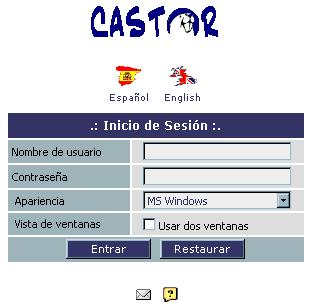
\includegraphics{./imagenes/castor/login.jpg}
  \caption[\small Pantalla de Inicio de sesi�n]
  {\small Pantalla de Inicio de sesi�n.}
  \label{figlogin}
\end{figure} 

Si el usuario ingresa el nombre de usuario o contrase�a de manera incorrecta, el sistema despliega un mensaje como el que se muestra en la figura \ref{figerrorlogin}.\\

\begin{figure}[!ht]
  \centering
  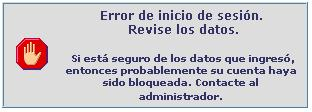
\includegraphics{./imagenes/castor/errorinicio.jpg}
  \caption[\small Mensaje de error de inicio de sesi�n]
  {\small Mensaje de error de inicio de sesi�n.}
  \label{figerrorlogin}
\end{figure}  

Si los datos provistos por el usuario son correctos, entonces se muestra la pantalla principal de la aplicaci�n, como se muestra en la figura \ref{figmain}. Esta pantalla est� compuesta por tres partes: el men� en la parte izquierda, la barra de funciones adicionales en la parte superior y los mensajes de ayuda (relacionados al tema del SQA) en la parte central.\\

\begin{figure}[!ht]
  \centering
  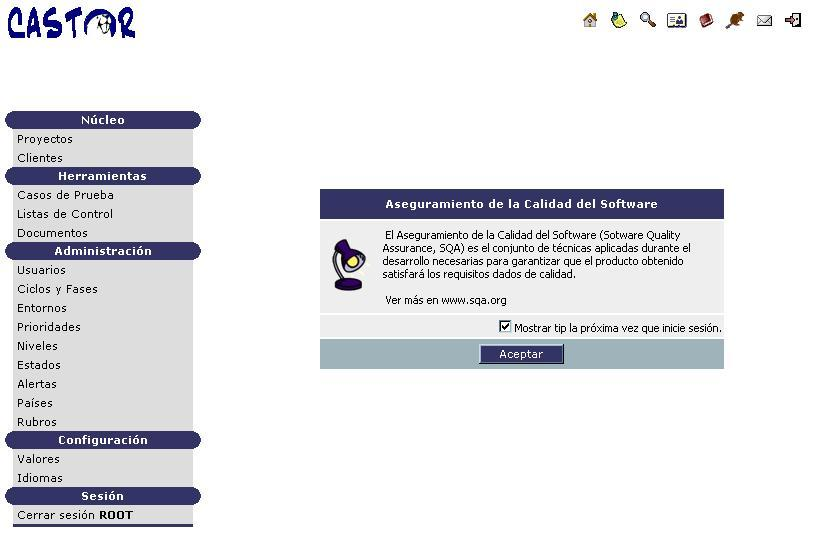
\includegraphics[width=\textwidth]{./imagenes/castor/main2.jpg}
  \caption[\small Pantalla principal de la aplicaci�n]
  {\small Pantalla principal de la aplicaci�n.}
  \label{figmain}
\end{figure}  
 
El men� principal conduce al usuario a las tareas m�s importantes que se pueden desempe�ar utilizando la herramienta, como la gesti�n de proyectos, clientes, casos de prueba, etc., adem�s de la gesti�n de entidades complementarias a las mencionadas, como estados, prioridades, entornos, ciclos y fases, etc.. La configuraci�n de la aplicaci�n es s�lo accesible para Administradores.\\

En la parte superior derecha se encuentran enlaces a funciones adicionales de la herramienta, como la administraci�n de la cuenta actual, el buscador, el acceso al documento de ayuda y el cierre de la sesi�n actual.\\
 
\begin{figure}[!ht]
  \centering
  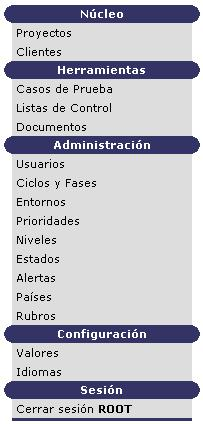
\includegraphics{./imagenes/castor/menu.jpg}
  \caption[\small Men� principal]
  {\small Men� principal.}
  \label{figmenu}
\end{figure}

\begin{figure}[!ht]
  \centering
  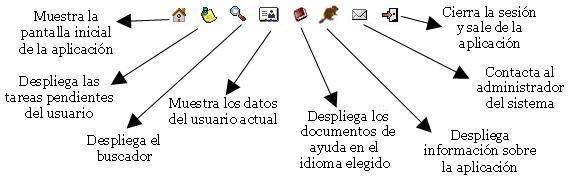
\includegraphics{./imagenes/castor/upbar.jpg}
  \caption[\small Barra de funciones adicionales]
  {\small Barra de funciones adicionales.}
  \label{figupbar}
\end{figure}

Cada ventana que es accedida desde los enlaces provistos en el men� posee en general las caracter�sticas descritas a continuaci�n.\\

	Una tabla que lista los registros de la entidad seleccionada. A manera de ejemplo, la figura \ref{figvtestcase} muestra la pantalla de administraci�n de Casos de Prueba.\\
 
\begin{figure}[!ht]
  \centering
  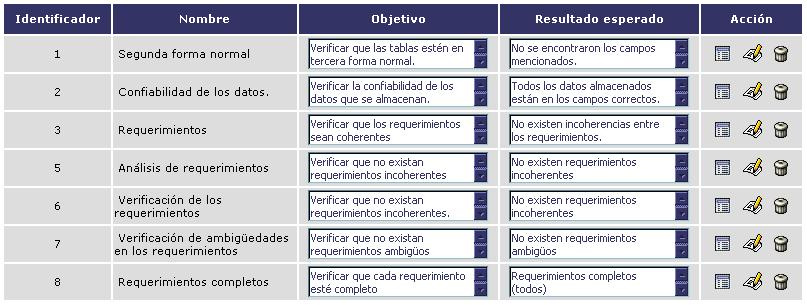
\includegraphics[width=\textwidth]{./imagenes/castor/vtestcase.jpg}
  \caption[\small Pantalla de administraci�n de casos de prueba]
  {\small Pantalla de administraci�n de casos de prueba.}
  \label{figvtestcase}
\end{figure}

	Junto a cada registro, se despliega un conjunto de iconos que conducen a distintas acciones a efectuar con �ste. Estas acciones se habilitan a cada usuario de acuerdo al rol que desempe�e (por ejemplo, un Desarrollador no puede ejecutar Casos de Prueba pero s� un Tester). La figura \ref{figiconos} muestra todos los iconos que aparecen en distintos lugares de la aplicaci�n y una breve descripci�n de la funci�n que cada uno tiene asociada.\\
 
\begin{figure}[!ht]
  \centering
  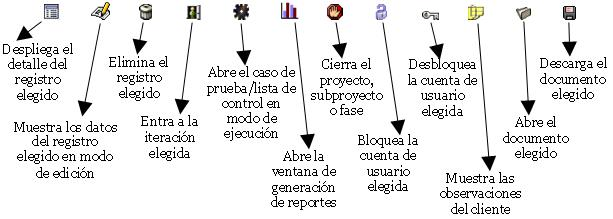
\includegraphics[width=\textwidth]{./imagenes/castor/iconos.jpg}
  \caption[\small Acciones disponibles para los registros]
  {\small Acciones disponibles para los registros.}
  \label{figiconos}
\end{figure}

	En el caso de que existan muchos registros para la entidad elegida, existen dos barras de navegaci�n entre p�ginas: una seg�n la p�gina y otra seg�n el orden alfab�tico (ver figura \ref{fignavigation}).\\

\begin{figure}[!ht]
  \centering
  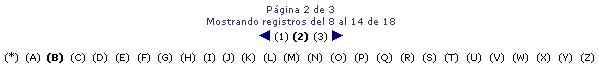
\includegraphics[width=\textwidth]{./imagenes/castor/navigation.jpg}
  \caption[\small Barras de navegaci�n entre registros de una misma entidad]
  {\small Barras de navegaci�n entre registros de una misma entidad.}
  \label{fignavigation}
\end{figure} 

A su vez, en la parte superior de la pantalla (debajo de la barra de funciones adicionales) se habilita la barra de navegaci�n entre partes de un proyecto (ver figura \ref{fignavigation2}) que cambia a medida que el usuario elige el proyecto, subproyecto, fase e iteraci�n con los que desea trabajar, lo que facilita el cambiar de nivel de detalle en cualquier momento sin necesidad de ir saliendo de manera secuencial de la iteraci�n, la fase, el subproyecto y el proyecto.\\

\begin{figure}[!ht]
  \centering
  
\includegraphics{./imagenes/castor/navigation2.jpg}
  \caption[\small Barra de navegaci�n entre partes de un proyecto]
  {\small Barra de navegaci�n entre partes de un proyecto.}
  \label{fignavigation2}
\end{figure} 

Los formularios de inserci�n y edici�n de datos poseen un robusto control de errores que ayudan al usuario a efectuar un correcto registro de la informaci�n, evitando as� posteriores problemas.\\
 
\begin{figure}[!ht]
  \centering
  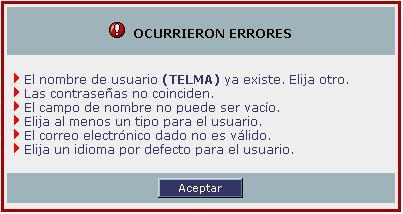
\includegraphics{./imagenes/castor/error.jpg}
  \caption[\small Ejemplo de mensaje de error durante el registro de un nuevo usuario]
  {\small Ejemplo de mensaje de error durante el registro de un nuevo usuario.}
  \label{figerror}
\end{figure} 

{\bfseries Tareas pendientes}\\

Cuando el usuario inicia la sesi�n y tiene tareas sin atender, el sistema le despliega un mensaje como el que se muestra en la figura \ref{figtareas}.

\begin{figure}[!ht]
  \centering
  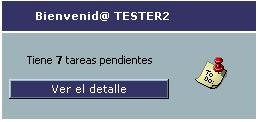
\includegraphics{./imagenes/castor/tareas.jpg}
  \caption[\small Mensaje de tareas pendientes]
  {\small Mensaje de tareas pendientes.}
  \label{figtareas}
\end{figure} 

El clic en el bot�n {\it Ver el detalle} conduce al usuario a una ventana con la lista de tareas pendientes, como se muestra en la figura \ref{figdetalletareas}.

\begin{figure}[!ht]
  \centering
  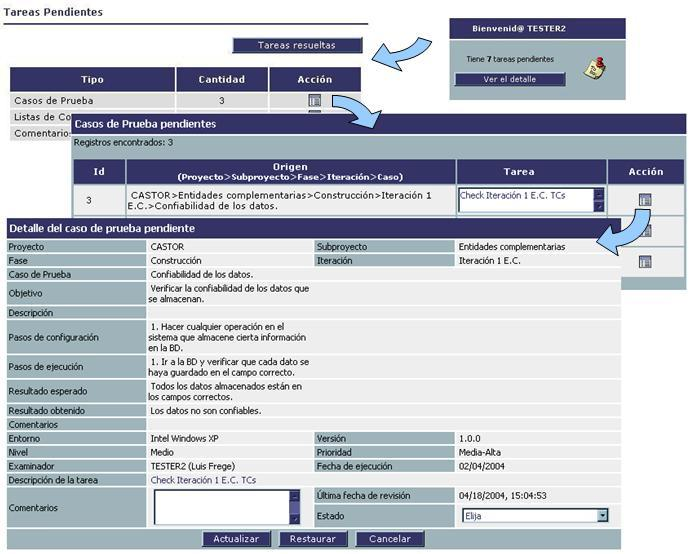
\includegraphics[width=\textwidth]{./imagenes/castor/detalletareas3.jpg}
  \caption[\small Detalle de tareas pendientes]
  {\small Detalle de tareas pendientes.}
  \label{figdetalletareas}
\end{figure} 

\subsection{Env�o de alertas}

Para el env�o de alertas se utilizan distintas tecnolog�as:
\begin{itemize}
\item Cron: programa residente en memoria que revisa cada minuto el archivo crontab. En este archivo se guardan las instrucciones que deben ser ejecutadas cada cierto periodo de tiempo (tambi�n indicado en el archivo).
\item PHP: se utilizan funciones del lenguaje para el env�o de alertas al correo electr�nico y tel�fono m�vil de cada usuario.
\item Servidor SMTP: se utiliza un servidor de correo electr�nico para el env�o de los correos (sin este servidor las instrucciones de PHP no funcionan.
\end{itemize}
El modo de trabajo entre estas tecnolog�as es el siguiente: el cron revisa cada minuto el archivo crontab en el que est� incluida la instrucci�n de ejecutar el script {\it enviar\_alertas.php} una vez al d�a. Cuando la instrucci�n es ejecutada, el script utiliza la funci�n {\it mail()} de PHP para enviar las alertas. Esta funci�n utiliza el servidor SMTP para despachar las alarmas. Si el env�o tuvo �xito, entonces el script almacena la fecha de env�o en la Base de Datos. La figura \ref{figenvioalertas} ilustra este modo de trabajo.

\begin{figure}[!ht]
  \centering
  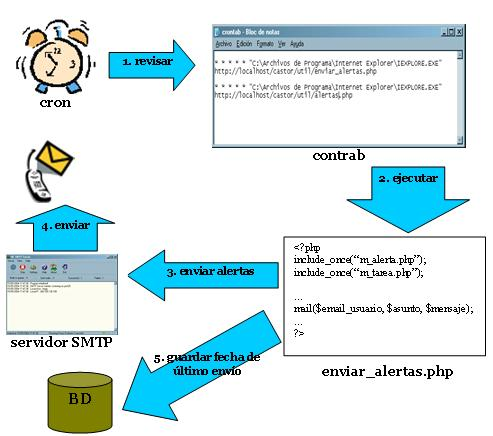
\includegraphics{./imagenes/castor/cron.jpg}
  \caption[\small Modo de env�o de alertas]
  {\small Modo de env�o de alertas utilizando el Cron, PHP y un servidor SMTP.}
  \label{figenvioalertas}
\end{figure} 

\subsection{Reportes}

Una de las partes m�s importantes del sistema son los reportes. �stos permiten la presentaci�n de la informaci�n contenida en la Base de Datos de manera objetiva, lo que ayuda al usuario en la toma de decisiones. Entre los m�s importantes la herramienta ofrece los siguientes:
\begin{itemize}
\item Porcentaje de avance de los subproyectos de un proyecto dependiendo de los resultados de las �ltimas iteraciones de cada una de sus fases.
\item Herramientas utilizadas por iteraci�n.
\item Tiempo que se demor� en cerrar una fase de un subproyecto, un subproyecto y un proyecto.
\item Cantidad de personas involucradas en el proceso de control de calidad de un proyecto (testers y desarrolladores).
\item Cantidad de errores encontrados por tester y cantidad de errores reportados a cada desarrollador.
\item Fases de un proyecto (de todos sus subproyectos) que tuvieron m�s iteraciones (es decir, qu� fases del proceso de desarrollo tuvieron m�s problemas durante el proceso de control de calidad).
\item Reporte completo sobre un proyecto, usuario o cliente en particular.
\item Desempe�o de los usuarios del sistema con respecto a sus tareas asignadas (estados de las tareas). Como ejemplo se muestra este reporte generado en la figura \ref{figreporte}.
\end{itemize}

\begin{figure}[!ht]
  \centering
  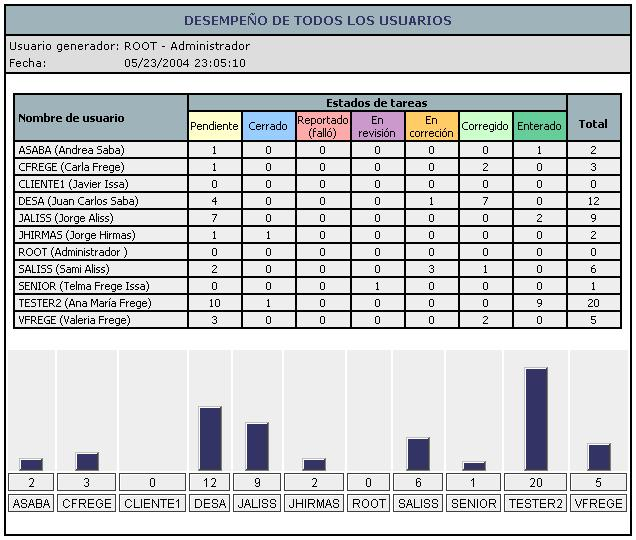
\includegraphics[width=\textwidth]{./imagenes/castor/reporte.jpg}
  \caption[\small Reporte generado por CASTOR]
  {\small Reporte generado por CASTOR: desempe�o de los usuarios.}
  \label{figreporte}
\end{figure} 

\subsection{Manuales}
\label{seccionmanuales}

La aplicaci�n ofrece como parte de la documentaci�n seis tipos de manuales:
\begin{itemize}
\item	Manual de Instalaci�n y Configuraci�n
\item	Manual del Administrador
\item	Manual del L�der de Proyectos
\item	Manual del Tester
\item	Manual del Desarrollador
\item	Manual del Cliente
\end{itemize}
Cada uno de los cuales explica al usuario -de acuerdo a su rol- las funciones que debe desempe�ar dentro del sistema y la manera en que �ste se comporta antes las distintas situaciones posibles. Estos manuales est�n en versi�n electr�nica (formato PDF) y son accesibles desde el icono de ayuda de la aplicaci�n. Tambi�n vienen incluidos en el CD que est� asjunto al documento principal de este proyecto.

\chapter{PRUEBAS}

Las pruebas efectuadas al sistema se clasifican en: pruebas de verificaci�n (``�se est� construyendo la herramienta de acuerdo a los requerimientos dados?'') y pruebas de validaci�n (``�se est� construyendo lo que el usuario necesita?'').

\section{Pruebas de verificaci�n}

\subsection{Pruebas de unidad}

Las pruebas de unidad se realizan concentrando la atenci�n en un m�dulo en particular. En ellas se verifica que cada m�dulo, de manera independiente, haga lo que debe hacer.\\

Estas pruebas fueron efectuadas dividiendo la aplicaci�n en las distintas entidades que la componen: proyectos, clientes, usuarios, casos de prueba, etc. y probando cada una de las funciones asociadas a estas entidades, como las de crear nuevo, modificar, eliminar, etc.\\

Las entidades fueron divididas en dos grupos b�sicos: ``entidades principales'' (proyectos, subproyectos, clientes, casos de prueba, listas de control, usuarios e iteraciones) y ``entidades complementarias'' (prioridades, estados, entornos, ciclos, fases, etc.). Estas �ltimas deben su nombre a la dependencia que tienen dentro del sistema de las primeras. Es decir, por s� solas no tienen utilidad en el sistema pero s� complementando la funcionalidad de las entidades principales (por ejemplo, la entidad ``estado'' complementa a las entidades iteraci�n, usuario, proyecto, etc.).\\

Debido a esta dependencia, las entidades complementarias fueron las primeras en ser desarrolladas y luego las entidades principales.

\subsection{Pruebas de integraci�n}

Las pruebas de integraci�n sirven para verificar que no existan problemas en la interacci�n entre uno o m�s m�dulos, que las funciones de un m�dulo no anulen o interrumpan las funciones de otro y que las funciones compartidas se ejecuten correctamente.\\

En este caso, las pruebas de integraci�n fueron ejecutadas de forma ascendente uniendo primero las entidades complementarias entre s� (como en el caso de ciclos y fases) y luego �stas a las principales a medida que las �ltimas eran desarrolladas. Luego se unieron las entidades principales entre s� para poder armar el flujo de trabajo ({\it workflow}) de la aplicaci�n.\\

Se realiz� una integraci�n ascendente debido a lo que ya se explic� en el anterior apartado: para poder desarrollar las entidades principales se requer�a contar con las complementarias listas. De la misma forma, para poder armar el flujo de trabajo, se requer�a contar con las entidades principales ya implementadas.\\

\subsection {Pruebas de Caja Blanca y Caja Negra}

	{\bfseries Pruebas de Caja Blanca}
	
	En las pruebas de verificaci�n de caja blanca, lo que interesa es comprobar que no existan sentencias en el c�digo que nunca sean ejecutadas (trozos de ``c�digo muerto'').	Este tipo de pruebas se efectu� con las entidades principales (las entidades secundarias tienen un menor volumen de c�digo y no requirieron de este tipo de verificaci�n).\\

	{\bfseries Pruebas de Caja Negra}

	En estas pruebas lo importante no es c�mo se ejecuta, sino que se obtenga lo que se desea. Son pruebas ajenas al c�digo involucrado durante la ejecuci�n, lo �nico que interesa es que la funci�n produzca el resultado esperado.\\
	
	Ambos tipos de pruebas se llevaron a cabo dentro de las pruebas de unidad y de integraci�n.\\
	
	{\bfseries Resultados\\}
	Los trozos de la aplicaci�n que fueron m�s dif�ciles de verificar a causa de la cantidad de c�digo involucrado fueron las iteraciones (incluida la ejecuci�n de casos de prueba y listas de control) y el control de tareas de los usuarios. Este gran volumen de c�digo se debe a la necesidad de extensos controles que deben ser ejecutados durante el uso de las iteraciones y las tareas. Estos controles, a su vez, son necesarios ya que en estas funciones se manipulan grandes cantidades de datos debido a que pr�cticamente todas las entidades, tanto principales como complementarias, se ven involucradas en la ejecuci�n -por ejemplo- de un caso de prueba en una iteraci�n de una fase del subproyecto de un proyecto.\\\\
	Los errores que se presentaban en estas secciones deb�an ser rastreados y corregidos, cuidando que los cambios hechos no afectaran a las dem�s funcionalidades que las mismas l�neas de c�digo pod�an desempe�ar. Sin embargo, el hecho de contar con la aplicaci�n implementada en MVC facilit� las tareas de identificaci�n de los puntos cr�ticos del c�digo que causaban problemas y la correcci�n inmediata de �stos.
	
\section{Pruebas de validaci�n}

Estas pruebas deben ser ejecutadas por los potenciales usuarios finales del sistema. Es decir, l�deres de proyectos, testers y desarrolladores.\\

\subsection{Pruebas Alfa}

Las pruebas Alfa son ejecutadas por los usuarios y el equipo de desarrollo a fin de validar que el software adquirido alcanz� los objetivos planteados inicialmente.\\\\
Estas pruebas fueron llevadas a cabo cuando el sistema fue concluido, validando que:
\begin{itemize}
\item Ofrezca soporte al control de la calidad del software durante todas las fases de un proyecto.
\item Sea amigable en su uso.
\item Permita la personalizaci�n de las herramientas ofrecidas (casos de prueba y checklists).
\end{itemize}
La herramienta obtenida cumple con los objetivos que se trazaron en un principio.

\subsection{Pruebas Beta - Aceptaci�n del Usuario}

Las pruebas de validaci�n Beta son ejecutadas por los usuarios finales del sistema, ajenas a todo lo que fue el desarrollo del producto.\\

Para la ejecuci�n de estas pruebas se recurri� a cinco empresas nacionales que est�n distribuidas en las tres ciudades principales del pa�s: Cochabamba, La Paz y Santa Cruz:

\begin{itemize}
\item Intersoft (La Paz)
\item Cybercia (Cochabamba)
\item BZDesigners (Santa Cruz)
\item E\&M Computadoras y Programas (Santa Cruz)
\item Axess Web (Santa Cruz)
\end{itemize}

Cada una de estas empresas (representadas para las pruebas por una a seis personas) particip� del ciclo de pruebas del sistema que consisti� en la presentaci�n del mismo mediante la ejecuci�n de un caso de ejemplo. Posteriormente, cada empresa tuvo a su disposici�n la aplicaci�n por un periodo de diez d�as.\\

Entre las opiniones emitidas hacia la aplicaci�n, se pueden mencionar:\\

\begin{quote}
{\it``Producto excelente que apoya el control de la calidad asegurando un proceso formal.''} {\small (Patricia Aguilar, Jefe de Sistemas Cybercia)}\\
\end{quote}

\begin{quote}
{\it``Herramienta de mucha utilidad para los procesos de desarrollo de software.''} {\small (Iv�n Monta�o, L�der de Proyectos  Intersoft)}\\
\end{quote}

\begin{quote}
{\it``Herramienta muy �til que, debidamente utilizada, resulta de gran ayuda para testear QA en SW.''} {\small (Carlos G�ngora, L�der de Proyectos Intersoft)}\\
\end{quote}

\begin{quote}
{\it``Bastante bueno, mejor que otras herramientas similares.''} {\small (Aldo Guti�rrez, desarrollador Intersoft)}\\
\end{quote}

\begin{quote}
{\it``Buen m�todo de seguimiento para el control de calidad. Bastante amigable en su uso.''} {\small (Fernando Vargas, desarrollador Intersoft)}\\
\end{quote}

\begin{quote}
{\it``Presenta grandes ventajas como herramienta de control de calidad. Adicionalmente, su flexibilidad en la configuraci�n de casos de prueba y listas de control hace que sea una herramienta muy completa.''} {\small (Octavio Alz�rreca, Jefe de proyectos Intersoft)}\\
\end{quote}

\begin{quote}
{\it``Simplifica y ordena el proceso de control de calidad.''} {\small (Sinchy D�az, desarrolladora Intersoft)}\\
\end{quote}

\begin{quote}
{\it``Excelente. �til, pr�ctico e independiente de la plataforma.''} {\small (Branko Zabala, Gerente General BZDesigners)}\\
\end{quote}

\begin{quote}
{\it``Bastante �til y necesaria para el desarrollo de software. Su flexibilidad permite a los usuarios definir sus propios par�metros de calidad.''} {\small (Pamela Pacheco, Jefe de Sistemas Axess Web)}\\
\end{quote}

\begin{quote}
{\it``Herramienta que viene a llenar un gran vac�o en el medio que en tiempo y materia econ�mica tiene un costo elevado. 100\% de aprobaci�n.''} {\small (Rub�n Salazar, E\&M Computadoras y Programas)}\\
\end{quote}


%``Los bugs se esconden en las esquinas y se congregan en los l�mites'' Boris Beizer


%http://www.itver.edu.mx/comunidad/material/ing-software/21


\chapter{CONCLUSIONES Y RECOMENDACIONES}

\section{Conclusiones}

\sloppy

\begin{enumerate}
\item La ausencia de aplicaci�n de m�todos formales de control de calidad ocasiona en la mayor�a de los casos retrasos en las entregas, fallas en los productos finales o incluso fracasos.
\item La Calidad de un producto es la coherencia que existe entre el software adquirido y los requerimientos fijados para �ste antes de su desarrollo, tanto expl�citos como impl�citos. Por lo tanto, la calidad de un software es tan importante como su funcionalidad.
\item Calidad no es sin�nimo de perfecci�n. Un producto de alta calidad no necesariamente estar� libre de errores. De hecho, el software libre de errores no existe, sino el que cumple con todos sus objetivos iniciales y con m�tricas bien definidas que se traducen en factores de calidad reconocidos.
\item Productos sometidos a procesos de control de calidad durante su desarrollo se traducen en uso eficiente de recursos y una alta probabilidad de terminar los planes a tiempo y cumpliendo con todos los objetivos propuestos.
\item Si el control de calidad se aplica desde las fases m�s tempranas del desarrollo, la cantidad de errores severos que se encuentran en las �ltimas fases se reduce de manera considerable.
\item Las empresas carentes de m�todos b�sicos de control de calidad y procesos maduros experimentan problemas que acarrean consigo una alta dependencia de personas imprescindibles, el riesgo elevado de contar con malos productos que, de terminarse, lo har�n utilizando m�s recursos de los previstos (tiempo, dinero, personas) y causando un deterioro progresivo de la imagen de la empresa ante la competencia y los clientes.
\item La calidad de un producto depende directamente del grado de compromiso que asuman las personas involucradas en su desarrollo.
\item Los modelos y est�ndares actuales deben ser utilizados como gu�as de orientaci�n y fuentes de potenciales soluciones a los problemas m�s comunes de las empresas.
\item Cualquier aplicaci�n de Control de Calidad disponible en la actualidad es tan eficiente como sus usuarios lo permitan. La definici�n personalizada de las herramientas (como los casos de prueba) causa que una aplicaci�n llegue a ser muy potente en su uso o completamente in�til, dependiendo del grado de aprovechamiento del usuario (testers sobretodo).
\item La manera m�s pr�ctica de implementar el SQA es la sistematizaci�n de sus herramientas: Casos de Prueba y Listas de Control.
\item CASTOR ofrece a los usuarios la posibilidad de implementar de manera formal las herramientas b�sicas del SQA (casos de prueba y listas de control), teniendo toda la informaci�n centralizada y estructurada.
\item La aplicaci�n obtenida permite la ejecuci�n de las herramientas mencionadas en todas las fases del desarrollo del producto.
\item El modelo de arquitectura MVC cumple con su objetivo principal: la reducci�n del esfuerzo invertido durante la implementaci�n.
\item La definici�n de un buen Marco de Trabajo para la implementaci�n del software simplifica el trabajo permitiendo el ahorro considerable del esfuerzo y los recursos invertidos. Adem�s, facilita la definici�n de convenciones de programaci�n, lo que a su vez contribuye a que el c�digo sea claro, eficiente, escalable y reparable.
\end{enumerate}


\section{Recomendaciones}

\begin{enumerate}
\item Profundizar la investigaci�n realizada tomando como base un Marco de Trabajo espec�fico y la manera en que �ste puede acomodarse a la realidad nacional. Por ejemplo, se puede estudiar la factiblidad de la aplicaci�n del modelo CMM en el �mbito local bajo ciertos criterios que el investigador considere oportunos.
\item Implementar un m�dulo (Interfaz) que permita al sistema la ejecuci�n semi autom�tica de Casos de Prueba.
\item Permitir que el sistema soporte iteraciones anidadas. 
\item Manejo de comunicaci�n m�s compleja entre los distintos usuarios del sistema. Por ejemplo, que permita la delegaci�n de subtareas entre desarrolladores.
\item Implementar un m�dulo que permita el seguimiento completo de los requerimientos durante el proceso de control de calidad.
\item Permitir que la aplicaci�n no s�lo implemente las herramientas del SQA (casos de prueba y checklists) sino tambi�n sus pr�cticas m�s recomendadas, como las RTFs.
\end{enumerate}

\clearpage
\chapter*{GLOSARIO}
\addcontentsline{toc}{chapter}{GLOSARIO}

{\bfseries Algoritmo}.- Secuencia finita de instrucciones dada para resolver un problema espec�fico. Cada una de estas instrucciones tiene un significado claro y es ejecutada con una cantidad de esfuerzo finita.\\

{\bfseries ANSI}.- El ``American National Standards Institute'', al igual que el SEI, la ISO y el IEEE, est� vinculado con la calidad mediante sus publicaciones de est�ndares.\\
		
{\bfseries API}.-	Application Programming Interface. Conjunto de rutinas o funciones que un programa puede utilizar para que el Sistema Operativo realice alguna tarea.\\
		
{\bfseries Caja Blanca, Testeo de}.- Conjunto de pruebas donde el tester es responsable de verificar la ejecuci�n de cada prueba hasta el m�s m�nimo nivel de detalle, incluyendo una revisi�n del c�digo involucrado.\\
		
{\bfseries Caja Gris, Testeo de}.- H�brido entre el testeo de caja blanca y el testeo de caja negra. El tester verifica el c�digo sin mucho nivel de detalle.\\
		
{\bfseries Caja Negra, Testeo de}.- Conjunto de pruebas donde lo �nico que interesa es verificar la funcionalidad y no as� la manera en que el programa ejecuta las tareas. Al tester no le interesa si el c�digo est� bien escrito, simplemente si la tarea es bien realizada o no.\\
		
{\bfseries CGI}.- Common Gateway Interface. Es un protocolo gen�rico que permite extender las capacidades de HTTP. Los programas CGI a�aden funcionalidad al servidor Web.\\
		
{\bfseries Cliente}.- Ordenador que funciona localmente y se comunica con el servidor para solicitar informaci�n.\\
		
{\bfseries Defecto}.- Anomal�a de un producto.\\
		
{\bfseries EIS}.- Enterprise Information System. Se refiere a cualquier sistema que proporciona una infraestructura para el soporte de la informaci�n de la empresa.\\
		
{\bfseries Escalabilidad}.- Es la medida en que un sistema es capaz de soportar y servir a m�s de un usuario, entendi�ndose como usuario a cualquier agente que haga uso del sistema, ya sea una persona como otro sistema.\\
		
{\bfseries Framework}.- Es la extensi�n de un lenguaje mediante una o m�s jerarqu�as de clases que implementan una funcionalidad y que (opcionalmente) pueden ser extendidas.\\
		
{\bfseries HTML}.- HiperText Markup Language. Conjunto de marcas (m�s conocidas como etiquetas o "tags" en ingl�s) que permite b�sicamente el formateo de documentos de hipertexto para su divulgaci�n en el World Wide Web.\\
		
{\bfseries HTTP}.- HiperText Transfer Protocol. Principal protocolo de Internet para la transferencia de archivos.\\
		
{\bfseries IEEE}.- ``Institute of Electrical and Electronics Engineers''. Entre otras publicaciones, se encuentra relacionado a la calidad del software mediante sus est�ndares ``IEEE Standard for Software Test Documentation'' (IEEE/ANSI 829), ``IEEE Standard of Software Unit Testing'' (IEEE/ANSI Standard 1008) y ``IEEE Standard for Software Quality Assurance Plans'' (IEEE/ANSI Standard 730).\\
		
{\bfseries IIS}.- El Internet Information Server es el conjunto de herramientas ofrecidas por Microsoft para la administraci�n y control de sitios Web, FTP, SMTP y Servicio de noticias. 
		
{\bfseries Interface}.- Parte de una aplicaci�n capaz de interactuar con el usuario.\\
		
{\bfseries ISO}.- ``Internacional Organization for Standarization''. Esta organizaci�n est� involucrada con la calidad mediante sus est�ndares 9001, 9002 y 9003.\\
		
{\bfseries L�gica del Negocio}.- Porci�n de la arquitectura realizada por componentes que es utilizada para crear y garantizar las reglas establecidas.\\
		
{\bfseries Proceso}.- Un proceso define qui�n hace qu�, cu�ndo y c�mo para lograr un objetivo. Es una secuencia de tareas b�sicas que alg�n individuo de la empresa desempe�a con el fin de alcanzar un objetivo.\\
		
{\bfseries SEI}.- ``Software Engineering Institute'' de la Universidad Carnegie Mellon de Pittsburgh Pennsylvania, Estados Unidos. Es el responsable del desarrollo del CMM� - Capability Madurity Model.\\
		
{\bfseries Servidor}.- Ordenador remoto (en alg�n lugar de la red) cuya tarea es proporcionar informaci�n a los clientes seg�n peticiones.\\
		
{\bfseries SGML}.- Standard Generalized Markup Language. \\
		
{\bfseries Shell}.- Interface de un programa. \\
		
{\bfseries Smalltalk}.- Lenguaje de programaci�n Orientado a Objetos que naci� como fruto de una investigaci�n de XEROX en 1972.\\
		
{\bfseries Tester}.- Persona encargada de hacer las pruebas al software.\\


\bibliography{./biblio/biblio}

\anexos
\renewcommand{\appendixname}{Anexo} 
\thispagestyle{empty}
\addcontentsline{toc}{chapter}{ANEXOS}

\linespread{1}

\chapter[EMPRESAS CERTIFICADAS POR LA ISO Y EL CMM�]{EMPRESAS CERTIFICADAS POR LA ISO Y EL CMM�}
\label{anexocertificaciones}
\setcounter{page}{1}

Origen de esta informaci�n: \cite{NAS2003}.

\setlength{\arrayrulewidth}{1pt}
\setlength{\doublerulesep}{0mm}

\begin{longtable}{|p{3in}|c|c|}
\hline\hline
{Empresa} & {ISO} & {CMM�}\\ 
\hline
%#s
\footnotesize 24/7 Customer.com	& \footnotesize 9002:1994 & \footnotesize \\
\footnotesize 3Com India Pvt Ltd & \footnotesize	9000 & \footnotesize \\ \hline

%A
\footnotesize A G Technologies Pvt Ltd & \footnotesize 9001:2000 & \footnotesize \\
\footnotesize Accel Software Solutions Limited	& \footnotesize 9001 & \footnotesize \\
\footnotesize Ace Software Exports Ltd	& \footnotesize 9002	& \footnotesize \\
\footnotesize Adroit Computer Technique Pvt Ltd & \footnotesize	9001:2000	 & \footnotesize \\
\footnotesize Aithent Technologies Pvt Ltd.	& \footnotesize & \footnotesize	Nivel 5 \\
\footnotesize Alcatel India Limited. & \footnotesize	9001	& \footnotesize \\
\footnotesize ALSTOM Systems Limited & \footnotesize	9001	& \footnotesize \\
\footnotesize American Express (India) Pvt. Ltd. & \footnotesize & \footnotesize	Nivel 2  \\
\footnotesize AmitySoft Technologies Pvt Ltd	& \footnotesize 9001:2000	 & \footnotesize \\
\footnotesize Ampersand Software Applications Ltd. & \footnotesize	9001	& \footnotesize \\
\footnotesize Apex Technologies Pvt. Ltd.	& \footnotesize 9001 & \footnotesize \\
\footnotesize Aptech Limited.	& \footnotesize 9001	& \footnotesize \\
\footnotesize Atos Origin India Private Limited	& \footnotesize 9001:2000	& \footnotesize Nivel 5 \\
\footnotesize Aviation Software Development Consultancy India Ltd.	& \footnotesize & \footnotesize	Nivel 3 \\
\footnotesize AXA Business Services Pvt Ltd	& \footnotesize 9002	& \footnotesize \\
\footnotesize Axes Technologies (I) Pvt Ltd	& \footnotesize 9001	& \footnotesize \\ \hline

%B
\footnotesize BAeHAL Software Limited	& \footnotesize 9001	& \footnotesize \\
\footnotesize Bangalore Software Services Ltd	& \footnotesize 9001	& \footnotesize \\
\footnotesize Bells Softech Limited	& \footnotesize 9001:1994	& \footnotesize \\
\footnotesize Beni Softwares Pvt Ltd & \footnotesize	9001:2000	 & \footnotesize \\
\footnotesize Bhari Information Technology Systems Pvt. Ltd.	& \footnotesize 9001	 & \footnotesize \\
\footnotesize Bharti Telesoft Ltd.	& \footnotesize 9001	& \footnotesize \\
\footnotesize Birla Technologies Ltd	& \footnotesize 9001	 & \footnotesize \\
\footnotesize Birlasoft Limited	& \footnotesize 9001	 & \footnotesize \\
\footnotesize Botree Software International Ltd	& \footnotesize 9001	 & \footnotesize \\
\footnotesize BPL Telecom Ltd. & \footnotesize	9001	& \footnotesize Nivel 3  \\
\footnotesize BT (Worldwide) Ltd.	& \footnotesize 9001	& \footnotesize \\ \hline

%C	
\footnotesize Canbank Computer Services Ltd. & \footnotesize 9001	 & \footnotesize \\
\footnotesize CA-TCG Software Pvt. Ltd. & \footnotesize	9001	 & \footnotesize \\
\footnotesize CDS International Ltd	& \footnotesize 9001	 & \footnotesize \\
\footnotesize Cellnext Solutions Ltd	& \footnotesize 9001:2000 & \footnotesize \\	 
\footnotesize Celstream Technologies Pvt Ltd	& \footnotesize 9001:2000	 & \footnotesize \\
\footnotesize Cerebra Integrated Technologies Ltd	& \footnotesize 9001:2000	 & \footnotesize \\
\footnotesize CG Maersk Information Technologies Pvt. Ltd. & \footnotesize 9001 & \footnotesize \\	 
\footnotesize CGI Information Systems and Management Consultants Pvt Ltd	& \footnotesize 9001 & \footnotesize	Nivel 4  \\
\footnotesize CG-Smith Software Limited	 & \footnotesize & \footnotesize	Nivel 5  \\
\footnotesize CG-VAK Software Exports Ltd.	& \footnotesize 9001	 & \footnotesize \\
\footnotesize Chandigarh Infotech Centre Ltd.	& \footnotesize 9001:2000	 & \footnotesize \\
\footnotesize Churchill India Pvt. Ltd.	& \footnotesize 9002 & \footnotesize \\
\footnotesize CMC Limited	& \footnotesize 9001:1994	& \footnotesize Nivel 3  \\
\footnotesize Cognizant Technology Solutions India Pvt. Ltd. & \footnotesize 9001	& \footnotesize Nivel 5 \\
\footnotesize Compudyne Winfosystems Limited	& \footnotesize 9001:2000	 & \footnotesize \\
\footnotesize Compulink Systems Pvt Ltd	& \footnotesize 9001 & \footnotesize \\
\footnotesize Computer Clinic India Pvt. Ltd.	& \footnotesize 9001	& \footnotesize \\
\footnotesize Congruent Solutions Pvt. Ltd.	& \footnotesize 9001	& \footnotesize \\
\footnotesize Consoliintd Cybernetics Co. Pvt. Ltd.	& \footnotesize 9001:2000	& \footnotesize \\
\footnotesize Consoliintd Futuristic Solutions Ltd	& \footnotesize 9001	& \footnotesize \\
\footnotesize Consulting Engineering Services (I) Ltd	& \footnotesize 9001	& \footnotesize \\
\footnotesize Contech Software Ltd.	& \footnotesize 9001	& \footnotesize \\
\footnotesize Convergent Software Limited	 & \footnotesize & \footnotesize Nivel 3  \\
\footnotesize Covansys India (Private) Ltd.	& \footnotesize 9001	& \footnotesize Nivel 5  \\
\footnotesize Crossword Software Pvt Ltd	& \footnotesize 9001	& \footnotesize \\ 
\hline

%D
\footnotesize Datamatics Ltd.	& \footnotesize 9001	& \footnotesize PCMM Nivel 2  \\
\footnotesize Datamatics Technologies Pvt. Ltd.	& \footnotesize 9001:2000	& \footnotesize PCMM Nivel 2  \\
\footnotesize DCM Datasystems Ltd. & \footnotesize	9001	& \footnotesize \\ 
\footnotesize DCM Technologies Limited	& \footnotesize & \footnotesize	Nivel 5  \\
\footnotesize DDE ORG Systems Ltd.	& \footnotesize & \footnotesize 9001:2000	 \\ 	
\footnotesize Differential Technologies Limited	& \footnotesize 9001	& \footnotesize \\
\footnotesize Digital GlobalSoft Ltd.	& \footnotesize 9001 & \footnotesize	Nivel 4 \\ 
\footnotesize Divine India Limited	& \footnotesize 9001:2000	 & \footnotesize \\
\footnotesize DPS Technologies India Pvt Ltd	& \footnotesize 9002:1994	 & \footnotesize \\
\footnotesize DSL Software Ltd.	& \footnotesize 9001	 & \footnotesize \\
\footnotesize DSQ Software Limited	& \footnotesize 9001	& \footnotesize Nivel 5  \\
\footnotesize DSS Infotech International Ltd.	& \footnotesize 9001	& \footnotesize \\
\footnotesize Duncan Infotech	& \footnotesize 9001	& \footnotesize \\
\footnotesize Dusk Valley Technologies Ltd	& \footnotesize 9001:2000	 & \footnotesize \\ \hline

%E
\footnotesize Eastern Software Systems Ltd. & \footnotesize	9001	& \footnotesize Nivel 5 \\
\footnotesize E-Brahma Technologies (P) Ltd. & \footnotesize	9001:1994	 & \footnotesize \\
\footnotesize eFunds International Private Limited & \footnotesize & \footnotesize	Nivel 3  \\
\footnotesize Eonour Software Ltd.	& \footnotesize 9001	 & \footnotesize \\
\footnotesize Eximsoft Technologies Pvt. Ltd.	& \footnotesize 9001	 & \footnotesize \\
\footnotesize EXplora InfoTech Limited	& \footnotesize 9001:2000	 & \footnotesize \\ 
\hline
		
%F
\footnotesize FCS Software Solutions Ltd & \footnotesize	9001	& \footnotesize \\
\footnotesize Financial Technologies (India) Ltd.	& \footnotesize 9001 & \footnotesize	Nivel 3 \\
\footnotesize Future Software Limited	& \footnotesize 9001:2000	& \footnotesize Nivel 5, PCMM Nivel 3 \\ 
\hline
	
%G	
\footnotesize GAVS Information Services Pvt. Ltd.	& \footnotesize 9001:2000	 & \footnotesize \\
\footnotesize Genisys Integrating Systems (I) Pvt. Ltd. & \footnotesize	9001 & \footnotesize \\
\footnotesize Global Dialnet Limited	& \footnotesize 9001 & \footnotesize \\
\footnotesize Global Infosystems Ltd	& \footnotesize 9001 & \footnotesize \\	 
\footnotesize Globalsoft Pvt. Ltd.	& \footnotesize 9001 & \footnotesize \\ 
\footnotesize Globsyn Technologies Ltd.	& \footnotesize 9001 & \footnotesize \\
\footnotesize Godrej Infotech Ltd	& \footnotesize 9001, 9002	& \footnotesize Nivel 4 \\
\footnotesize Goldstone Technologies Ltd	& \footnotesize 9001:2000 & \footnotesize \\
\footnotesize Growth Compusoft Exports Ltd.	& \footnotesize 9002 & \footnotesize \\
\footnotesize GTL Limited	& \footnotesize 9001:2000	& \footnotesize Nivel 4  \\ 
\hline

%H
\footnotesize HCL Infosystems Ltd	& \footnotesize 9001 & \footnotesize Nivel 4 \\
\footnotesize HCL Perot Systems Pvt Ltd	 & \footnotesize 9001 & \footnotesize	Nivel 5 \\
\footnotesize HCL Technologies Ltd	& \footnotesize 9001	& \footnotesize Nivel 5  \\
\footnotesize Hewlett-Packard (India) Software Operations Pvt Ltd & \footnotesize	9001:2000 & \footnotesize	Nivel 5 \\
\footnotesize Hexaware Technologies Limited	& \footnotesize 9001	& \footnotesize Nivel 5 \\
\footnotesize Hinduja TMT Ltd	& \footnotesize 9001:1994	 & \footnotesize \\
\footnotesize Honeywell India Software Operations Pvt. Ltd. & \footnotesize	9001 & \footnotesize	Nivel 4 \\ 
\footnotesize HTC Software Development Centre & \footnotesize	9001	& \footnotesize Nivel 3 \\
\footnotesize Hughes Software Systems Ltd	9001 & \footnotesize & \footnotesize Nivel 4 \\
\hline

%I
\footnotesize i2 Technologies India Pvt. Ltd.	& \footnotesize  9001 & \footnotesize \\
\footnotesize IBILT Technologies Ltd.	& \footnotesize  9001:9002	 & \footnotesize \\
\footnotesize IBM Global Services India Pvt. Ltd.	& \footnotesize  9001:2000	& \footnotesize Nivel 5 \\
\footnotesize ICICI Infotech Services Ltd.	& \footnotesize  9001	& \footnotesize Nivel 3 \\
\footnotesize iCope Technologies Private Limited	& \footnotesize  9001 & \footnotesize \\
\footnotesize Ideaspace Solutions Ltd.	& \footnotesize 9001:2000	 & \footnotesize \\
\footnotesize i-flex solutions ltd.	 & \footnotesize & \footnotesize	Nivel 5 \\
\footnotesize IIS Scientific Computing Ltd	& \footnotesize 9001:2000	 & \footnotesize \\
\footnotesize India Education Centre Softwares Limited	 & \footnotesize 9001	& \footnotesize \\
\footnotesize Indus Software Pvt. Ltd. & \footnotesize 9001	 & \\
\footnotesize Infinite Computer Solutions (India) Pvt. Ltd.	 & 	& \footnotesize Nivel 3 \\
\footnotesize Information Technologies (India) Limited	 & \footnotesize 9001 & \footnotesize Nivel 5 \\
\footnotesize Information Technology Park Ltd.	&\footnotesize 9000	& \footnotesize \\
\footnotesize Infosys Technologies Ltd.	 & \footnotesize 9001 & \footnotesize Nivel 5 \\
\footnotesize Infotech Enterprises Ltd.	& \footnotesize 9001,9002 & \footnotesize Nivel 5 \\
\footnotesize Infozech Software (P) Ltd.	& \footnotesize 9001	& \footnotesize \\
\footnotesize InfraSoft Technologies Limited	 & \footnotesize 9001:2000	& \footnotesize \\
\footnotesize Intelligroup Asia Pvt. Ltd.	& \footnotesize 9001	& \footnotesize Nivel 5, PCMM Nivel 2 \\
\footnotesize InteQ Software Limited	 & \footnotesize 9001	  & \\
\footnotesize IonIdea Enterprise Solutions Pvt Ltd	 & \footnotesize 9001	& \footnotesize Nivel 3  \\
\footnotesize iS3C Consultancy Services Ltd. & \footnotesize 9001	& \footnotesize Nivel 4 \\
\footnotesize iSeva Systems Pvt Ltd	 & \footnotesize 9001:2000	  & \\
\footnotesize IT Solutions (India) Pvt. Ltd. & \footnotesize 9001	& \footnotesize Nivel 5  \\
\footnotesize ITC Infotech India Ltd	 & \footnotesize 9001	& \footnotesize Nivel 5  \\
\footnotesize ITTI Limited  & \footnotesize 9001	  & \\
\footnotesize Ivega Corporation	 & \footnotesize 9001	& \footnotesize Nivel 4 \\
\footnotesize IVL India Pvt. Ltd.	 & \footnotesize 9001	  & \\
\hline
	
%J
\footnotesize JK Technosoft Ltd	 & \footnotesize 9001	  & \\
\footnotesize JP Mobile (India) Limited	 & \footnotesize 9001:2000	  & \\
\hline

%K
\footnotesize Kale Consultants Pvt. Ltd.	 & \footnotesize 9001	  & \\
\footnotesize Kals Information Systems Ltd	 & \footnotesize 9001	  & \\
\footnotesize Kanbay Software (India) Pvt. Ltd.	 & \footnotesize 9001:1994	  & \\
\footnotesize Kaneriya Technologies Limited	& 9002	  & \\
\footnotesize Karvy Consultants Ltd	& 9002	  & \\
\footnotesize Keane India Ltd	 & \footnotesize 9001	& \footnotesize Nivel 5 \\
\footnotesize KLG Systel Ltd.	 & \footnotesize 9001  & \\
\footnotesize KPIT Infosystems Limited.	 & \footnotesize 9001	& \footnotesize Nivel 4 \\
\hline

%L		
\footnotesize Larsen and Toubro Infotech Limited	 & \footnotesize 9001:2000	& \footnotesize Nivel 4  \\
\footnotesize LG Soft India Pvt. Ltd.	 & \footnotesize 9001	& \footnotesize Nivel 5 \\
\footnotesize Linc Software Services Pvt. Ltd.	 & \footnotesize 9001:1994	  & \\
\footnotesize Live Tech Solutions (P) Ltd	 & \footnotesize 9000	  & \\
\footnotesize Lucent Technologies India (P) Ltd.	 & \footnotesize 9001	  & \\
\hline

%M	
\footnotesize Magic Software Pvt. Ltd.	 & \footnotesize 9001	  & \\
\footnotesize Mahindra British Telecom Ltd.	 & \footnotesize 9001	& \footnotesize Nivel 3 \\
\footnotesize Majoris Systems Pvt. Ltd.	 & \footnotesize 9001	  & \\
\footnotesize MASCON Global Limited	 & \footnotesize 9000	  & \\
\footnotesize Mascot Systems Ltd.	 & \footnotesize 9001:2000	CMM� & \footnotesize Nivel 4 \\
\footnotesize MASTEK Ltd.	 & \footnotesize 9001	& \footnotesize PCMM Nivel 3, Nivel 5  \\
\footnotesize MECON Limited	 & \footnotesize 9001	  & \\
\footnotesize Medicom Solutions (P) Ltd	 & \footnotesize 9001	  & \\
\footnotesize Megasoft Limited	 & \footnotesize 9001:1994	  & \\
\footnotesize Melstar Information Technologies Ltd	 & \footnotesize 9001:2000	& \footnotesize Nivel 3  \\
\footnotesize Micro Technologies (India) Ltd	 & \footnotesize 9001:1994	 & \\
\footnotesize Mindteck (India) Ltd	 & \footnotesize 9001:1994	 & \\
\footnotesize Momentum India Private Limited	 & \footnotesize 9001	  & \\
\footnotesize Motorola India Electronics Private Ltd.	 &	& \footnotesize Nivel 5 \\
\footnotesize Mphasis BFL Ltd.	 & \footnotesize 9001	& \footnotesize Nivel 5 \\
\footnotesize MTC (India) Pvt. Ltd.	 & \footnotesize 9001:2000	  & \\
\hline

%N	
\footnotesize NatureSoft Private Limited	 & \footnotesize 9001	  & \\
\footnotesize Navayuga Infotech Pvt. Ltd.	 & \footnotesize 9001	  & \\
\footnotesize Neptune Information Solutions Limited	 & \footnotesize 9001	  & \\
\footnotesize Network Programs (India) Ltd. &	 	& \footnotesize Nivel 3 \\
\footnotesize Network Systems and Technologies (P) Ltd.	 & \footnotesize 9001	& \footnotesize Nivel 5  \\
\footnotesize Newgen Imaging Systems (P) Ltd.	 & \footnotesize 9001	  & \\
\footnotesize NIIT Ltd.	 & \footnotesize 9001	& \footnotesize Nivel 5  \\
\footnotesize Nokia Telecommunications Pvt. Ltd.	 & \footnotesize 9000	  & \\
\hline
	
%O
\footnotesize Onward Technologies Limited	 & 9002	  & \\
\footnotesize Opusasia Technologies Pvt. Ltd	 & \footnotesize 9001	  & \\
\footnotesize Oracle India Private Limited.	 & \footnotesize 9001	& \footnotesize Nivel 4 \\
\footnotesize Oracle Solution Services (India) Pvt Ltd	 & \footnotesize 9001	& \footnotesize Nivel 4  \\
\footnotesize OrbiTech Solutions Limited	& 	& \footnotesize Nivel 5  \\
\footnotesize Orient Information Technology Ltd.	& 9002	  & \\
\hline

%P		
\footnotesize Paharpur Business Centre	& 9002	  & \\
\footnotesize Paragon Solutions (I) Pvt. Ltd.	 	& & \footnotesize Nivel 3 \\
\footnotesize Patni Computer Systems Ltd.	 & \footnotesize 9001:2000	& \footnotesize Nivel 5 \\
\footnotesize Pentamedia Graphics Limited	 & \footnotesize 9001	& \footnotesize Nivel 4 \\
\footnotesize Pentasoft Technologies Limited	 & \footnotesize 9001	& \footnotesize Nivel 4 \\
\footnotesize Philips Software Centre Pvt. Ltd.	 & \footnotesize 9001	& \footnotesize Nivel 5 \\
\footnotesize Phoenix Global Solutioins (India) Pvt. Ltd.	 & \footnotesize 9001	  & \\
\footnotesize Planet PCI Infotech Ltd	 & \footnotesize 9001	  & \\
\footnotesize PlanetAsia.com Limited	 	& & \footnotesize Nivel 4  \\
\footnotesize Polaris Software Lab Ltd & \footnotesize 9001	& \footnotesize CMMI Nivel 5 \\
\footnotesize Premier Technology Group Pvt. Ltd.	 & \footnotesize 9001	  & \\
\footnotesize Princeton Software Exports Pvt. Ltd.	 & \footnotesize 9001:2000	  & \\
\footnotesize PSI Data Systems Ltd.	 & \footnotesize 9001	  & \\
\footnotesize Pyxis Technology Solutions Ltd	 & \footnotesize 9001	  & \\
\hline

%Q	
\footnotesize QAI (India) Limited	 	&  & \footnotesize PCMM Nivel 2 \\
\footnotesize Quinnox Consultancy Services Ltd	 &	& \footnotesize Nivel 5 \\
\hline

%R
\footnotesize R S Software (India) Ltd.	 & \footnotesize 9001 & \footnotesize	PCMM Nivel 3, Nivel 4  \\
\footnotesize R Systems International Limited	 & \footnotesize 9001:2000 & \footnotesize Nivel 4  \\
\footnotesize Ram Informatics Ltd.	 & \footnotesize 9001	  & \\
\footnotesize Ramco Systems Ltd	 & \footnotesize 9001:1994	  & \\
\footnotesize RelQ Software Pvt Ltd	 & \footnotesize 9001:2000	  & \\
\footnotesize Resonance Technologies (P) Ltd.	 & \footnotesize 9001	  & \\
\footnotesize Rishabh Software Pvt Ltd	 & \footnotesize 9001:2000 & \\	 
\footnotesize River Run Software Group	 & \footnotesize 9001	 & \\ 
\footnotesize Robert BOSCH India Limited & \footnotesize 9001:1994 & \footnotesize Nivel 3   \\
\footnotesize Rolta India Ltd.  & \footnotesize 9001:2000	  & \\
\hline
	
%S	
\footnotesize SAP India Pvt. Ltd.	 & \footnotesize 9001,9002	 & \\ 
\footnotesize Sar Softech Pvt Ltd	 & \footnotesize 9001	  & \\
\footnotesize Sasken Communication Technologies Limited	 & \footnotesize 9001:1994 & \\	 
\footnotesize Satyam Computer Services Ltd.	 & \footnotesize 9001:2000	& \footnotesize Nivel 5  \\
\footnotesize Selectronic Equipment and Services Pvt. Ltd.	 & \footnotesize 9002	  & \\
\footnotesize Shyama Software Solutions (I) Pvt Ltd	 & \footnotesize 9001	  & \\
\footnotesize Siemens Information Systems Ltd.	 & \footnotesize 9001	& \footnotesize Nivel 5, PCMM Nivel 3 \\
\footnotesize Siemens Public Communications Network Ltd.	 & \footnotesize 9001	  & \\
\footnotesize Sierra Optima Ltd.	 & \footnotesize 9001:2000 & \\	 
\footnotesize Silverline Technologies Ltd.	 & \footnotesize 9001	& \footnotesize Nivel 4 \\
\footnotesize Siri Technologies Private Limited	 & \footnotesize 9001	  & \\
\footnotesize Sitel India Pvt Ltd	 & \footnotesize 9000	  & \\
\footnotesize Softek Limited	 & \footnotesize 9001:1994 & \\
\footnotesize Solitar Systems (India) Pvt Ltd	 & \footnotesize 9001:2000	  & \\
\footnotesize SolutionNET India (Pvt ) Ltd	 & \footnotesize 9001:2000	  & \\
\footnotesize Sonata Software Limited	 & \footnotesize 9001	& \footnotesize Nivel 5  \\
\footnotesize Sovika Infotek Ltd.	 & \footnotesize 9001	  & \\
\footnotesize Speck Systems Limited	 & \footnotesize 9001	  & \\
\footnotesize SQL Star International Limited	 & \footnotesize 9001:2000& \\
\footnotesize SRA Systems Ltd.	 & \footnotesize 9001	& \footnotesize Nivel 4  \\
\footnotesize Srishti Software Private Limited	& & \footnotesize Nivel 3	  \\
\footnotesize SSI Technologies	 & \footnotesize 9001,9002	& \footnotesize Nivel 5  \\
\footnotesize Subex Systems Limited	 & \footnotesize 9001	 & \\
\footnotesize Summit Information Technologies Ltd	 & \footnotesize 9001:2000	& \\
\footnotesize Syntel (India) Ltd.	 & \footnotesize 9001	& \footnotesize Nivel 5 \\
\footnotesize Systems and Software	 & \footnotesize 9001	  & \\
\hline

%T	
\footnotesize Tata Consultancy Services	 & \footnotesize 9001	& \footnotesize Nivel 5, PCMM Nivel 4 \\
\footnotesize Tata Elxsi (India) Ltd.	 & \footnotesize 9001,9002	& \footnotesize Nivel 5  \\
\footnotesize Tata Infotech Ltd.	 & \footnotesize 9001,9002	& \footnotesize Nivel 4  \\
\footnotesize Tata Interactive Systems	 & \footnotesize 9001	& \footnotesize Nivel 5  \\
\footnotesize Tata Technologies Limit ed	 & \footnotesize 9001:2000	  & \\
\footnotesize TCG Software Services Pvt. Ltd.	 & \footnotesize 9001	  & \\
\footnotesize TCIL BellSouth Ltd.	 & \footnotesize 9001	  & \\
\footnotesize TechSpan India Ltd.	 &	& \footnotesize PCMM Nivel 3  \\
\footnotesize Tektronix Engineering Development (I) Ltd.	 & \footnotesize 9000:2001 & \\	 
\footnotesize Telecommunications Consultants India Ltd.	 & \footnotesize 9001	  & \\
\footnotesize Temenos India Pvt. Ltd.	 & \footnotesize 9000	 & \\
\footnotesize Thermax Systems and Software	 & \footnotesize 9001 & \\	 
\footnotesize Three S Solutions Ltd	 & \footnotesize 9002	 & \\ 
\footnotesize Trident Infotech Corporation Ltd.	 & \footnotesize 9001:2000 & \\
\footnotesize Trigent Software Ltd.	 & \footnotesize 9001	& \\
\hline
		
%U
\footnotesize UshaComm India Pvt. Ltd.	 & \footnotesize 9001	  & \\
\footnotesize Ushus Technologies Pvt Ltd	 & \footnotesize 9001	  & \\
\hline

%V	
\footnotesize Value Software Technologies Pvt. Ltd.	 & \footnotesize 9001	  & \\
\footnotesize Visesh Infosystems Limited	 & \footnotesize 9001	  & \\
\footnotesize Vispark Solutions (I) Pvt Ltd	 & \footnotesize 9001	  & \\
\footnotesize VJIL Consulting Limited	 & \footnotesize 9001	 & \\ 
\footnotesize VXL eTech Ltd	 	& & \footnotesize Nivel 3  \\
\hline

%W	
\footnotesize Web Spiders (I) Pvt Ltd	 & \footnotesize 9001	  & \\
\footnotesize Webify Services (India) Private Limited	 & \footnotesize 9001	  & \\
\footnotesize West Bengal Electronics Industry Development Corporation Ltd.	 & \footnotesize 9002	  & \\
\footnotesize Wipro Technologies	 & \footnotesize 9001	& \footnotesize Nivel 5 \\
\footnotesize WNS Global Services	 & \footnotesize 9001	 & \\
\hline
	
%X	
\footnotesize Xansa (India) Ltd	 & \footnotesize 9001	& \footnotesize Nivel 5 \\
\footnotesize Xcelvision Technologies Limited	 & \footnotesize 9001:2000	 & \\
\footnotesize Xerox Modicorp Limited	& 	& \footnotesize Nivel 3 \\
\hline

%Z	
\footnotesize Zenith Computers Ltd.	 &  \footnotesize 9000	 & \\
\footnotesize Zensar Technologies Limited	 & \footnotesize 9001	& \footnotesize Nivel 5, EFQM Nivel 2 \\
\hline\hline

\caption{Empresas certificadas por la ISO y el CMM�}\\ 
\end{longtable} 

\clearpage 

\chapter{CASOS DE PRUEBA Y LISTAS DE CONTROL}
\label{anexocasospruebachecklists}

Los siguientes son modelos de casos de prueba y extractos de listas de control basadas en las que William Lewis presenta en su libro {\it Software Testing and Continuous Quality Improvement.} \cite{LEW2000}.\\

{\bfseries \large Caso de Prueba}

\begin{figure}[!ht]
  \centering
  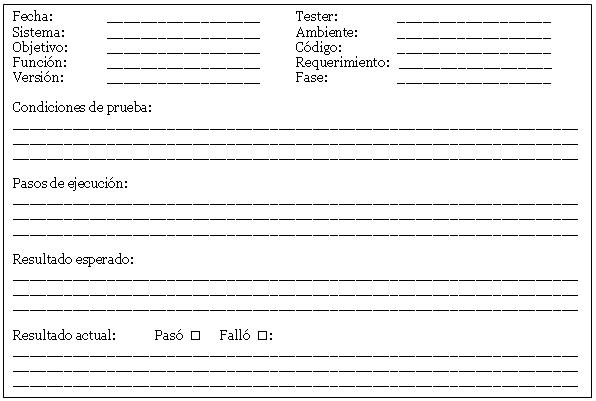
\includegraphics{./imagenes/anexos/casoprueba.jpg}
  \caption[\small Modelo de Caso de Prueba]{\small Modelo de Caso de Prueba \cite{LEW2000}.}
  \label{figcasoprueba}
\end{figure}

\clearpage

{\bfseries \large Listas de Control}\\

{\small S�: La sentencia se cumple.\\}
{\small No: La sentencia no se cumple.\\}
{\small Om: La sentencia fue omitida.\\}
{\small NP: La sentencia a�n no fue probada.\\}

	\begin{enumerate}
	
	\item {\bfseries Fase de requerimientos}

\setlength{\arrayrulewidth}{1pt}
\setlength{\doublerulesep}{0mm}

\begin{longtable}{|p{4.5in}|c|c|c|c|}
\hline
{\footnotesize Defecto} & {\footnotesize S�} & {\footnotesize No} &
{\footnotesize Om} & {\footnotesize NP}\\ 
\hline		
\footnotesize 1. La l�gica del negocio est� siendo utilizada inadecuadamente. & & & & \\	 
\footnotesize 2. El criterio para el performance est� siendo mal utilizado.	 & & & & \\
\footnotesize 3. La informaci�n del entorno es err�nea, insuficiente o irrelevante.	 	 	 	  & & & & \\
\footnotesize 4. El objetivo del sistema no ha sido bien planteado.	 	 	 	  & & & & \\
\footnotesize 5. Los requerimientos son incompatibles.	 	 	 	  & & & & \\
\footnotesize 6. Los requerimientos son incompletos.	 	 	 	  & & & & \\
\footnotesize 7. Faltan algunos requerimientos.	 	 	 	  & & & & \\
\footnotesize 8. Los requerimientos son err�neos.	 	 	 	  & & & & \\
\footnotesize 9. La exactitud especificada no est� conforme con la necesidad actual. & & & & \\
\footnotesize 10. El entorno de los datos no est� descrito de forma adecuada.	 	& & & & \\
\footnotesize 11. La definici�n de interfaces externas es err�nea.	 	 	 	  & & & & \\
\footnotesize 12. El entrenamiento para el usuario no ha sido bien considerado.	 	 	 	 & & & & \\ 
\footnotesize 13. El estado del sistema al ser inicializado no ha sido bien considerado.	 & & & & \\
\footnotesize 14. Las funciones no han sido bien definidas.	  & & & & \\ 
\footnotesize 15. Las necesidades del usuario no han sido bien planteadas.	 & & & & \\
\footnotesize 16. Las m�tricas de calidad no han sido bien especificadas.	 & & & & \\	 	 
\hline
\caption{Criterios a considerar en el testeo de requerimientos}
\end{longtable} 
	
	\item {\bfseries Fase de dise�o l�gico}
	
	
\setlength{\arrayrulewidth}{1pt}
\setlength{\doublerulesep}{0mm}

\begin{longtable}{|p{4.5in}|c|c|c|c|}
\hline
{\footnotesize Defecto} & {\footnotesize S�} & {\footnotesize No} &
{\footnotesize Om} & {\footnotesize NP}\\ 
\hline		
\footnotesize 1. Los datos no han sido definidos apropiadamente. & & & & \\
\footnotesize 2. La definici�n de la entidad est� incompleta.	 & & & & \\
\footnotesize 3. La cardinalidad de la entidad es incorrecta.	 & & & & \\
\footnotesize 4. Los atributos de la entidad est�n incompletos.	& & & & \\
\footnotesize 5. La normalizaci�n no es correcta.	& & & & \\
\footnotesize 6. La clave principal no es correcta.	& & & & \\
\footnotesize 7. La clave for�nea no es correcta.	& & & & \\
\footnotesize 8. La clave compuesta no es correcta.	 & & & & \\
\footnotesize 9. El sub-tipo de la entidad es incorrecto.	& & & & \\
\footnotesize 10. El proceso no ha sido bien definido. & & & & \\
\footnotesize 11. Los ``procesos padre'' no est�n bien definidos / est�n incompletos. & & & & \\
\footnotesize 12. Los ``procesos hijo'' no est�n bien definidos / est�n incompletos. & & & & \\
\footnotesize 13. Las salidas/entradas no est�n bien definidas.	 & & & & \\
\footnotesize 14. Los procesos elementales no est�n bien definidos.	& & & & \\
\footnotesize 15. Existe el problema de exclusi�n mutua.	& & & & \\
\footnotesize 16. La activaci�n de eventos no est� bien definida.	 & & & & \\
\footnotesize 17. La creaci�n de asociaciones entre entidades/procesos es incorrecta.	 & & & & \\
\footnotesize 18. La lectura de asociaciones entre entidades/procesos es incorrecta. & & & & \\
\footnotesize 19. La actualizaci�n de asociaciones entre entidades/procesos es incorrecta.& & & & \\
\footnotesize 20. La eliminaci�n de asociaciones entre entidades/procesos es incorrecta. & & & & \\
\hline
\caption{Criterios a considerar en el testeo del dise�o l�gico de la aplicaci�n}\\ 
\end{longtable}
	
	\item {\bfseries Fase de dise�o f�sico}
	
\begin{longtable}{|p{4.5in}|c|c|c|c|}
\hline
{\footnotesize Defecto} & {\footnotesize S�} & {\footnotesize No} &
{\footnotesize Om} & {\footnotesize NP}\\ 
\hline		
\footnotesize 1. La l�gica y/o secuencia es err�nea.& & & & \\
\footnotesize 2. El procesamiento es inexacto.& & & & \\
\footnotesize 3. Una rutina no tiene requisitos de entrada/salida.& & & & \\
\footnotesize 4. La rutina no acepta los datos con los rangos establecidos.& & & & \\
\footnotesize 5. La validaci�n est� hecha en los datos de entrada.& & & & \\
\footnotesize 6. Los procedimientos no son los adecuados.& & & & \\
\footnotesize 7. Falta un procesamiento correcto.& & & & \\
\footnotesize 8. Los valores son err�neos o ambiguos.& & & & \\
\footnotesize 9. Los datos almacenados son inadecuados.& & & & \\
\footnotesize 10. Faltan algunas variables.& & & & \\
\footnotesize 11. Los requerimientos de dise�o han sido malinterpretados / no est�n presentes.& & & & \\
\footnotesize 12. La Base de Datos no es compatible con el entorno de los datos.& & & & \\
\footnotesize 13. La descomposici�n modular refleja una alta dependencia intermodular.& & & & \\
\footnotesize 14. Los algoritmos m�s importantes no han sido evaluados en funci�n de su exactitud y velocidad.& & & & \\
\footnotesize 15. La estructura de control no es extensible.& & & & \\
\footnotesize 
16. La estructura de control omite las prioridades de procesamiento.& & & & \\
\footnotesize 17. Los protocolos de las interfaces son incorrectos.& & & & \\
\footnotesize 18. La l�gica utilizada para la implementaci�n de los algoritmos es incorrecta.& & & & \\
\footnotesize 19. Los datos no son formateados de la forma correcta.& & & & \\
\footnotesize 20. No se han considerado los efectos del trunqueo de datos. & & & & \\
\footnotesize 21. Los �ndices no son validados.& & & & \\
\footnotesize 22. Se permiten ciclos infinitos.& & & & \\
\footnotesize 23. La especificaci�n de los m�dulos ha sido malinterpretada.& & & & \\
\footnotesize 24. Las reglas de la Base de Datos han sido violadas.& & & & \\
\footnotesize 25. La l�gica est� incompleta para todos los casos.& & & & \\
\footnotesize 26. Los casos especiales son ignorados.& & & & \\
\footnotesize 27. El manejo de errores es deficiente.& & & & \\
\footnotesize 28. Las consideraciones de tiempo han sido ignoradas.& & & & \\
\footnotesize 29. Los requerimientos han sido cambiados en los m�dulos.& & & & \\
\footnotesize 30. Las especificaciones de las interfaces han sido malinterpretadas.& & & & \\
\footnotesize 31. El sistema funciona bien pero no cumple con los requerimientos de performance.& & & & \\
\footnotesize 32. El sistema no es lo suficientemente completo como para satisfacer la necesidad planteada.& & & & \\
\footnotesize 33. El ``overflow'' de operaciones aritm�ticas no ha sido considerado apropiadamente.& & & & \\
\footnotesize 34. Las acciones para las entradas dadas no son correctas.& & & & \\
\footnotesize 35. La aproximaci�n de los algoritmos no provee una exactitud adecuada.& & & & \\
\footnotesize 36. Existen errores en el dise�o detallado para resolver un problema en particular.& & & & \\
\footnotesize 37. Existen casos particulares de entradas cuyo resultado luego de un procesamiento es una salida no considerada.& & & & \\
\footnotesize 38. Existen algoritmos que pueden ser reemplazados por otros m�s eficientes.& & & & \\
\hline
\caption{Criterios a considerar en el testeo del dise�o f�sico de la aplicaci�n}
\end{longtable}
	
	\item {\bfseries Fase de dise�o de unidad de programa}
	
\begin{longtable}{|p{4.5in}|c|c|c|c|}
\hline
{\footnotesize Defecto} & {\footnotesize S�} & {\footnotesize No} &
{\footnotesize Om} & {\footnotesize NP}\\ 
\hline		
\footnotesize 1. �Las estructuras ``if-then-else'' son usadas correctamente?& & & & \\
\footnotesize 2. �Los ciclos (``while'', ``for'') son utilizados correctamente?& & & & \\
\footnotesize 3. �Existen ciclos infinitos?& & & & \\
\footnotesize 4. �El programa es f�cilmente legible?& & & & \\
\footnotesize 5. �El programa es eficiente?& & & & \\
\footnotesize 6. �Las estructuras ``case'' contemplan todos los casos?& & & & \\
\footnotesize 7. �Existe trozos de ``c�digo muerto''?& & & & \\
\footnotesize 8. �Los algoritmos est�n bien escritos?& & & & \\
\footnotesize 9. �Existen demasiadas anidaciones?& & & & \\
\footnotesize 10. �Existen expresiones booleanas demasiado complejas?& & & & \\
\hline
\caption{Criterios a considerar en el testeo del dise�o de unidad de programa}
\end{longtable}
	
	\item {\bfseries Fase de implementaci�n}
	
\begin{longtable}{|p{4.5in}|c|c|c|c|}
\hline
{\footnotesize Defecto} & {\footnotesize S�} & {\footnotesize No} &
{\footnotesize Om} & {\footnotesize NP}\\ 
\hline		
\footnotesize 1. La l�gica para la toma de decisiones es inadecuada.& & & & \\
\footnotesize 2. Los c�lculos aritm�ticos son err�neos.& & & & \\
\footnotesize 3. Las ramificaciones est�n mal.& & & & \\
\footnotesize 4. Existen ciclos infinitos porque est�n mal definidos.& & & & \\
\footnotesize 5. Las reglas del lenguaje de programaci�n son violadas.& & & & \\
\footnotesize 6. Los est�ndares de programaci�n no son respetados.& & & & \\
\footnotesize 7. Existen errores de typeo.& & & & \\
\footnotesize 8. Existen errores en el formato de las entradas y salidas.& & & & \\
\footnotesize 9. Existen errores en la invocaci�n a otros programas.& & & & \\
\footnotesize 10. Existen errores en los datos.& & & & \\
\footnotesize 11. Existen subprogramas inconclusos.& & & & \\
\footnotesize 12. El manejo de errores es incorrecto.& & & & \\
\footnotesize 13. Existen errores en el procesamiento de datos para las salidas.& & & & \\
\footnotesize 14. Existen errores en las interfaces.& & & & \\
\footnotesize 15. Existen errores de sintaxis.& & & & \\
\footnotesize 16. Existen errores de inicializaci�n.& & & & \\
\footnotesize 17. Existe confusi�n en el uso de los par�metros.& & & & \\
\footnotesize 18. Los contadores en los ciclos no funcionan correctamente.& & & & \\
\footnotesize 19. El resultado de las decisiones que se toman no es manejado correctamente.& & & & \\
\footnotesize 20. Los nombres de las variables no son apropiados.& & & & \\
\footnotesize 21. Las librer�as a utilizar no est�n claramente definidas.& & & & \\
\footnotesize 22. El tratamiento de caracteres especiales es incorrecto.& & & & \\
\footnotesize 23. Existen errores de compilaci�n.& & & & \\
\footnotesize 24. Existen problemas de ``overflow''.& & & & \\
\footnotesize 25. El software para interactuar con el hardware no funciona correctamente.& & & & \\
\footnotesize 26. Hay problemas a la hora de modificar los registros de la Base de Datos.& & & & \\
\hline
\caption{Criterios a considerar en el testeo de la fase de implementaci�n de la aplicaci�n}
\end{longtable}	

	\item {\bfseries Fase de pruebas}

\begin{longtable}{|p{4.5in}|c|c|c|c|}
\hline
{\footnotesize Defecto} & {\footnotesize S�} & {\footnotesize No} &
{\footnotesize Om} & {\footnotesize NP}\\ 
\hline		
\footnotesize 1. �Los c�digos son validados correctamente?& & & & \\
\footnotesize 2. �Los campos pueden ser actualizados sin problemas?& & & & \\
\footnotesize 3. �El largo de los campos es el adecuado?& & & & \\
\footnotesize 4. �La descripci�n de los campos es adecuada?& & & & \\
\footnotesize 5. �Los campos son inicializados correctamente?& & & & \\
\footnotesize 6. �Todas las referencias a un campo determinado son correctas?& & & & \\
\footnotesize 7. �Las restricciones de cada campo son validadas correctamente?& & & & \\
\footnotesize 8. �Existe un control de errores que verifique que las reglas establecidas sean respetadas?& & & & \\
\footnotesize 9. Para valores num�ricos, �se hace un control de valores positivos y negativos?& & & & \\
\footnotesize 10. Para valores alfanum�ricos, �el caso de ``vac�o'' ha sido contemplado?& & & & \\
\footnotesize 11. �Los propietarios de la informaci�n han testeado estos casos?& & & & \\
\footnotesize 12. �Los propietarios de la informaci�n han otorgado el resultado de sus pruebas?& & & & \\
\hline
\caption{Criterios a considerar en el testeo de la aplicaci�n en la fase de pruebas}
\end{longtable}
	
	\end{enumerate}


\chapter{ESPECIFICACI�N DE REQUERIMIENTOS Y PLAN DE PRUEBAS}
\label{anexoespecificacionrequerimientos}

{\bfseries \large Especificaci�n de Requerimientos}

El siguiente modelo es el recomendado por el IEEE y fue extra�do del libro de William Lewis (2000).

\renewcommand{\labelenumi}{%
 \theenumi.-
} 
\renewcommand{\theenumii}{\arabic{enumii}}
\renewcommand{\labelenumii}{%
 \theenumi.\theenumii.-
}

\renewcommand{\theenumiii}{\arabic{enumiii}}
\renewcommand{\labelenumiii}{%
 \theenumi.\theenumii.\theenumiii.-
}

\begin{enumerate}
\item Introducci�n
	\begin{enumerate}
	\item	Prop�sito
	\item	Alcance
	\item	Definiciones: Acr�nimos y Abreviaciones
	\item	Referencias
	\item	Resumen
	\end{enumerate}
\item	Descripci�n general
	\begin{enumerate}
	\item	Perspectiva del producto
		\begin{enumerate}
		\item	Interfaces del sistema
		\item	Interfaces de usuario
		\item	Interfaces del Hardware
		\item	Interfaces del Software
		\item	Comunicaci�n entre las interfaces
		\item	Limitaciones de memoria
		\item	Operaciones
		\item	Requerimientos de adaptaci�n
		\end{enumerate}
	\item	Funciones del producto
	\item	Caracter�sticas del usuario
	\item	Limitaciones
	\item	Suposiciones y Dependencias.
	\item	Reparto de Requerimientos
	\end{enumerate}
\item	Especificaci�n de Requerimientos
	\begin{enumerate}
	\item	Requerimientos de la Interface Externa
		\begin{enumerate}
		\item	Interfaces de usuario
		\item	Interfaces del Hardware
		\item	Interfaces del Software
		\item	Interfaces de comunicaci�n
		\end{enumerate}	
	\item Caracter�sticas del Sistema
		\begin{enumerate}
		\item	Caracter�stica 1
			\begin{enumerate}
			\item Introducci�n/Objetivo de la caracter�stica.
			\item Secuencia Est�mulo/Respuesta
			\item Requerimientos funcionales asociados
			\end{enumerate}	
		\item Caracter�stica 2
		\item ...
		\end{enumerate}	
	\item Requerimientos de Performance
	\item Limitantes del Dise�o
	\item Atributos del Software
	\item Otros Requerimientos
	\end{enumerate}
\item	Informaci�n de soporte
	\begin{enumerate}
	\item Tabla de Contenidos
	\item Ap�ndices\\
	\end{enumerate}
\end{enumerate}

\clearpage

{\bfseries \large Plan de Pruebas}

\begin{enumerate}
\item	Introducci�n
	\begin{enumerate}
	\item	Estrategia de testeo.
	\item Alcance del testeo.
	\end{enumerate}
\item	Testeo est�tico
	\begin{enumerate}
	\item Defectos descubiertos y corregidos
	\item Ideas de mejora
	\item Est�ndares del lenguaje utilizado.
	\item Est�ndares de la documentaci�n del desarrollo.
	\end{enumerate}
\item	Casos de Testeo (Testeo din�mico)
	\begin{enumerate}
	\item Datos de entrada
	\item Condiciones iniciales
	\item Resultados esperados
	\item Historial
	\end{enumerate}
\item	Requerimientos del entorno
	\begin{enumerate}
	\item Estrategia de testeo
	\item Plataforma
	\item Librer�as
	\item Herramientas
	\item Procedimientos
	\item Reportes
	\end{enumerate}
\end{enumerate}
 

\clearpage 

\chapter{DIAGRAMAS Y FUNCIONES}
\label{anexodiagramasyfunciones}

En este anexo se detallan los diagramas (casos de uso, colaboraci�n, estado y secuencia) y funciones que el sistema desempe�ar� organizados seg�n el tipo de usuario.\\

\begin{enumerate}

%%%%%%%%%%%%%%%%%%%%%%%%%%%%%%%%%%%%%%%%%%%%%%%%%%%%%%%%%%%%%%%%%%%%%%%%%%%%%%%%%%%%%%%%
%%%%%%%%%%%%%%%%%%%%%%%%%%%% G	E	N	�	R	I	C	O %%%%%%%%%%%%%%%%%%%%%%%%%%%%%%%%%%%%%%%%%%
%%%%%%%%%%%%%%%%%%%%%%%%%%%%%%%%%%%%%%%%%%%%%%%%%%%%%%%%%%%%%%%%%%%%%%%%%%%%%%%%%%%%%%%%

\item {\bfseries Usuario Gen�rico}

	\begin{enumerate}
	
	\item Diagrama de casos de uso

\begin{figure}[!ht]
  \centering
  \includegraphics{./imagenes/anexos/casesusuario.jpg}
  \caption[\small Diagrama de casos de uso detallado para un usuario gen�rico del sistema]
  {\small Diagrama de casos de uso detallado para un usuario gen�rico del sistema.}
\end{figure}
 
	 \item Funciones y diagramas de colaboraci�n, estado y secuencia

% USUARIO GEN�RICO
% FUNCI�N INGRESO

\begin{longtable}{|p{1in}|p{4.5in}|}
\hline 
\footnotesize {\bfseries Funci�n:}	& \footnotesize {\bfseries Ingreso de un usuario al sistema}\\
\footnotesize Descripci�n: &	\footnotesize Esta funci�n permite al usuario ingresar al sistema luego de registrar sus datos.\\
\footnotesize Entrada: &	\footnotesize Nombre de usuario y contrase�a pertenecientes al usuario.\\
\footnotesize Fuente:	& \footnotesize Usuario\\
\footnotesize Salida:	& \footnotesize Pantalla principal de la herramienta si los datos son correctos. Ventana de aviso de error en caso contrario.\\
\footnotesize Destino:	& \footnotesize El mismo usuario.\\
\footnotesize Precondici�n: &	\footnotesize Que el usuario tenga una cuenta creada en el sistema.\\
\hline
\end{longtable} 

\begin{figure}[!ht]
  \centering
  \includegraphics{./imagenes/anexos/colaboracionusuario1.jpg}
  \caption[\small Diagrama de colaboraci�n para la funci�n ``ingresar al sistema'']
  {\small Diagrama de colaboraci�n para la funci�n ``ingresar al sistema''.}
\end{figure}

\begin{figure}[!ht]
  \centering
  \includegraphics{./imagenes/anexos/estadosusuario1.jpg}
  \caption[\small Diagrama de estados para la funci�n ``ingresar al sistema'']
  {\small Diagrama de estados para la funci�n ``ingresar al sistema''.}
\end{figure}

\begin{figure}[!ht]
  \centering
  \includegraphics[width=15cm]{./imagenes/anexos/secuenciausuario1.jpg}
  \caption[\small Diagrama de secuencia para la funci�n ``ingresar al sistema'']
  {\small Diagrama de secuencia para la funci�n ``ingresar al sistema''.}
\end{figure}


% USUARIO GEN�RICO
% FUNCI�N ELECCI�N DEL IDIOMA
\clearpage

\begin{longtable}{|p{1in}|p{4.5in}|}
\hline 
\footnotesize {\bfseries Funci�n:}	& \footnotesize {\bfseries Elecci�n del idioma}\\
\footnotesize Descripci�n: &	\footnotesize Esta funci�n permite al usuario la elecci�n del idioma con el que desea trabajar en la sesi�n que iniciar�.\\
\footnotesize Entrada: &	\footnotesize Identificador del idioma a utilizar.\\
\footnotesize Fuente:	& \footnotesize Usuario (sin importar el tipo).\\
\footnotesize Salida:	& \footnotesize La aplicaci�n en el idioma elegido.\\
\footnotesize Destino:	& \footnotesize El mismo usuario.\\
\footnotesize Precondici�n: &	\footnotesize .\\
\hline
\end{longtable} 

\begin{figure}[!ht]
  \centering
  \includegraphics{./imagenes/anexos/colaboracionelegiridioma.jpg}
  \caption[\small Diagrama de colaboraci�n para la funci�n de ``elegir idioma'']
  {\small Diagrama de colaboraci�n para la funci�n de ``elegir idioma''.}
\end{figure}

\begin{figure}[!ht]
  \centering
  \includegraphics{./imagenes/anexos/estadosidioma.jpg}
  \caption[\small Diagrama de estados para la funci�n ``elegir idioma'']
  {\small Diagrama de estados para la funci�n ``elegir idioma''.}
\end{figure}

\begin{figure}[!ht]
  \centering
  \includegraphics[width=15cm]{./imagenes/anexos/secuenciausuario1.jpg}
  \caption[\small Diagrama de secuencia para la funci�n ``elegir idioma'']
  {\small Diagrama de secuencia para la funci�n ``elegir idioma''.}
\end{figure} 

% USUARIO GEN�RICO
% FUNCIONES GENERACION DE LISTADOS Y REPORTES
\clearpage

\begin{longtable}{|p{1in}|p{4.5in}|}
\hline 
\footnotesize {\bfseries Funci�n:}	& \footnotesize {\bfseries Generaci�n de listados}\\
\footnotesize Descripci�n: &	\footnotesize Esta funci�n permite la generaci�n de listados en los que desplegar� la informaci�n contenida en la Base de Datos hasta el momento con respecto a la opci�n seleccionada.\\
\footnotesize Entrada: &	\footnotesize La entidad elegida para generar el listado (ej.: usuarios, proyectos, casos de testeo, etc.).\\
\footnotesize Fuente:	& \footnotesize L�der de Proyectos, Tester, Administrador, Desarrollador.\\
\footnotesize Salida:	& \footnotesize Listado.\\
\footnotesize Destino:	& \footnotesize Gerencia, Equipo de testers, Equipo de desarrolladores, L�der del proyecto.\\
\footnotesize Precondici�n: &	\footnotesize Que el criterio dado cuente con informaci�n en la Base de Datos.\\
\hline
\end{longtable} 

\begin{longtable}{|p{1in}|p{4.5in}|}
\hline 
\footnotesize {\bfseries Funci�n:}	& \footnotesize {\bfseries Generaci�n de reportes}\\
\footnotesize Descripci�n: &	\footnotesize Esta funci�n permite la generaci�n de reportes en los que desplegar� la informaci�n contenida en la Base de Datos hasta el momento con respecto a la entidad seleccionada.\\
\footnotesize Entrada: &	\footnotesize La entidad elegida y los criterios que intervendr�n en la generaci�n del reporte.\\
\footnotesize Fuente:	& \footnotesize L�der de Proyectos, Administrador, Tester o Desarrollador.\\
\footnotesize Salida:	& \footnotesize Reporte.\\
\footnotesize Destino:	& \footnotesize Gerencia, Equipo de testers, Equipo de desarrolladores, L�der del proyecto.\\
\footnotesize Precondici�n: &	\footnotesize Que los criterios dados sean coherentes y se cuente con informaci�n en la Base de Datos.\\
\hline
\end{longtable} 

\begin{figure}[!ht]
  \centering
  \includegraphics{./imagenes/anexos/colaboracionusuario2.jpg}
  \caption[\small Diagrama de colaboraci�n para las funciones ``generaci�n de listados'' y ``generaci�n de reportes'']
  {\small Diagrama de colaboraci�n para las funciones ``generaci�n de listados'' y ``generaci�n de reportes''.}
\end{figure}
		
\begin{figure}[!ht]
  \centering
  \includegraphics{./imagenes/anexos/estadosusuario2.jpg}
  \caption[\small Diagrama de estados para las funciones ``generaci�n de listados'' y ``generaci�n de reportes'']
  {\small Diagrama de estados para las funciones ``generaci�n de listados'' y ``generaci�n de reportes''.}
\end{figure}

\begin{figure}[!ht]
  \centering
  \includegraphics[width=15cm]{./imagenes/anexos/secuenciausuario1.jpg}
  \caption[\small Diagrama de secuencia para las funciones ``generaci�n de listados'' y ``generaci�n de reportes'']
  {\small Diagrama de secuencia para las funciones ``generaci�n de listados'' y ``generaci�n de reportes''.}
\end{figure} 

% USUARIO GEN�RICO
% FUNCIONES GENERACION DE LISTADOS Y REPORTES
\clearpage

\begin{longtable}{|p{1in}|p{4.5in}|}
\hline 
\footnotesize {\bfseries Funci�n:}	& \footnotesize {\bfseries Cambio de datos personales}\\
\footnotesize Descripci�n: &	\footnotesize Esta funci�n permite al usuario modificar algunos de sus datos personales.\\
\footnotesize Entrada: &	\footnotesize Nuevos datos.\\
\footnotesize Fuente:	& \footnotesize Usuario (sin importar el tipo).\\
\footnotesize Salida:	& \footnotesize Modificaci�n de datos en la Base de Datos.\\
\footnotesize Destino:	& \footnotesize Base de Datos, usuario que gener� la acci�n.\\
\footnotesize Precondici�n: &	\footnotesize Que los nuevos datos sean v�lidos.\\
\hline
\end{longtable} 

\begin{figure}[!ht]
  \centering
  \includegraphics[width=\textwidth]{./imagenes/anexos/colaboracioncambiardatos.jpg}
  \caption[\small Diagrama de colaboraci�n para la funci�n ``cambio de datos personales'']
  {\small Diagrama de colaboraci�n para la funci�n ``cambio de datos personales''.}
\end{figure}
		
\begin{figure}[!ht]
  \centering
  \includegraphics{./imagenes/anexos/estadoscambiardatos.jpg}
  \caption[\small Diagrama de estados para la funci�n ``cambio de datos personales'']
  {\small Diagrama de estados para la funci�n ``cambio de datos personales''.}
\end{figure}

\begin{figure}[!ht]
  \centering
  \includegraphics[width=15cm]{./imagenes/anexos/secuenciacambiardatos.jpg}
  \caption[\small Diagrama de secuencia para la funci�n ``cambio de datos personales'']
  {\small Diagrama de secuencia para la funci�n ``cambio de datos personales''.}
\end{figure} 

% USUARIO GEN�RICO
% FUNCIONES GENERACION DE LISTADOS Y REPORTES
\clearpage

\begin{longtable}{|p{1in}|p{4.5in}|}
\hline 
\footnotesize {\bfseries Funci�n:}	& \footnotesize {\bfseries Cierre de la sesi�n}\\
\footnotesize Descripci�n: &	\footnotesize Funci�n que permite al usuario cerrar su sesi�n y salir de la aplicaci�n.\\
\footnotesize Entrada: &	\footnotesize Acci�n del usuario.\\
\footnotesize Fuente:	& \footnotesize Usuario (sin importar el tipo).\\
\footnotesize Salida:	& \footnotesize Eliminaci�n de las variables de sesi�n y cierre de la aplicaci�n.\\
\footnotesize Destino:	& \footnotesize Usuario que origin� la acci�n.\\
\footnotesize Precondici�n: &	\footnotesize Ninguna.\\
\hline
\end{longtable} 

\begin{figure}[!ht]
  \centering
  \includegraphics{./imagenes/anexos/colaboracioncerrarsesion.jpg}
  \caption[\small Diagrama de colaboraci�n para la funci�n ``cierre de sesi�n'']
  {\small Diagrama de colaboraci�n para la funci�n ``cierre de sesi�n''.}
\end{figure}
		
\begin{figure}[!ht]
  \centering
  \includegraphics{./imagenes/anexos/estadoscierresesion.jpg}
  \caption[\small Diagrama de estados para la funci�n ``cierre de sesi�n'']
  {\small Diagrama de estados para la funci�n ``cierre de sesi�n''.}
\end{figure}

\begin{figure}[!ht]
  \centering
  \includegraphics{./imagenes/anexos/secuenciacierresesion.jpg}
  \caption[\small Diagrama de secuencia para la funci�n ``cierre de sesi�n'']
  {\small Diagrama de secuencia para la funci�n ``cierre de sesi�n''.}
\end{figure} 

				\end{enumerate}



%%%%%%%%%%%%%%%%%%%%%%%%%%%%%%%%%%%%%%%%%%%%%%%%%%%%%%%%%%%%%%%%%%%%%%%%%%%%%%%%%%%%%%%%
%%%%%%%%%%%%%%%%%% A	D	M	I	N	I	S	T	R	A	D	O	R %%%%%%%%%%%%%%%%%%%%%%%%%%%%%%%%%%%%%%%%%%
%%%%%%%%%%%%%%%%%%%%%%%%%%%%%%%%%%%%%%%%%%%%%%%%%%%%%%%%%%%%%%%%%%%%%%%%%%%%%%%%%%%%%%%%
\clearpage

\item {\bfseries Usuario Administrador}
		
			\begin{enumerate}
			
			\item	Diagrama de casos de uso

\begin{figure}[!ht]
  \centering
  \includegraphics[width=15cm]{./imagenes/anexos/casesadministrador.jpg}
  \caption[\small Diagrama de casos de uso detallado para un usuario de tipo Administrador]
  {\small Diagrama de casos de uso detallado para un usuario de tipo Administrador.}
\end{figure} 
 
			\item Funciones y diagramas de colaboraci�n, estado y secuencia

\begin{longtable}{|p{1in}|p{4.5in}|}
\hline 
\footnotesize {\bfseries Funci�n:}	& \footnotesize {\bfseries Gesti�n de entidades complementarias}\\
\footnotesize Descripci�n: & \footnotesize 	Esta funci�n hace referencia a las acciones de inserci�n, modificaci�n y eliminaci�n de todas las entidades complementarias del sistema (ej: prioridades, entornos, estados, etc.).\\
\footnotesize Entrada: & \footnotesize Nombre de la entidad, acci�n requerida.\\
\footnotesize Fuente:	& \footnotesize Usuario.\\
\footnotesize Salida: &	\footnotesize Listado de los registros de la entidad, formulario de edici�n o mensaje de confirmaci�n de eliminaci�n (depende de la acci�n elegida).\\
\footnotesize Destino: & \footnotesize Base de Datos, Ventana del usuario.\\
\footnotesize Precondici�n: &	\footnotesize Que el usuario sea de tipo Administrador o Tester.\\
\hline
\end{longtable} 

\begin{longtable}{|p{1in}|p{4.5in}|}
\hline 
\footnotesize {\bfseries Funci�n:}	& \footnotesize {\bfseries Gesti�n de usuarios}\\
\footnotesize Descripci�n: &	\footnotesize Esta funci�n hace referencia a las acciones de inserci�n, modificaci�n, eliminaci�n bloqueo y desploqueo de los usuarios del sistema.\\
\footnotesize Entrada: &	\footnotesize Datos del usuario\\
\footnotesize Fuente:	& \footnotesize Usuario.\\
\footnotesize Salida: &	\footnotesize Registro en la Base de Datos del nuevo usuario. Ventana de detalle para el usuario que lo cre�.\\
\footnotesize Destino: & \footnotesize Base de Datos, Ventana del usuario.\\
\footnotesize Precondici�n: &	\footnotesize Que el usuario sea de tipo Administrador.\\
\hline
\end{longtable} 

\begin{figure}[!ht]
  \centering
  \includegraphics{./imagenes/anexos/colaboracionadmi1.jpg}
  \caption[\small Diagrama de colaboraci�n para las funciones ``gestionar entidades complementarias'' y ``gestionar usuarios'']
  {\small Diagrama de colaboraci�n para las funciones ``gestionar entidades complementarias'' y ``gestionar usuarios''. Caso: inserci�n de nuevo objeto.}
\end{figure} 

\begin{figure}[!ht]
  \centering
  \includegraphics[width=15cm]{./imagenes/anexos/estadosadmi1.jpg}
  \caption[\small Diagrama de estado para las funciones ``gestionar entidades complementarias'' y ``gestionar usuarios'']
  {\small Diagrama de estado para las funciones ``gestionar entidades complementarias'' y ``gestionar usuarios''. Caso: inserci�n de nuevo objeto.}
\end{figure} 

\begin{figure}[!ht]
  \centering
  \includegraphics[width=15cm]{./imagenes/anexos/secuenciaadmi1.jpg}
  \caption[\small Diagrama de secuencia para las funciones ``gestionar entidades complementarias'' y ``gestionar usuarios'']
  {\small Diagrama de secuencia para las funciones ``gestionar entidades complementarias'' y ``Gestionar usuarios''. Caso: inserci�n de nuevo objeto.}
\end{figure} 

\clearpage

\begin{longtable}{|p{1in}|p{4.5in}|}
\hline 
\footnotesize {\bfseries Funci�n:}	& \footnotesize {\bfseries Gesti�n de clientes}\\
\footnotesize Descripci�n: &	\footnotesize Esta funci�n hace referencia a las acciones de inserci�n, modificaci�n y eliminaci�n de clientes en el sistema.\\
\footnotesize Entrada: &	\footnotesize Datos del cliente.\\
\footnotesize Fuente:	& \footnotesize Usuario.\\
\footnotesize Salida: &	\footnotesize Modificaci�n del Cliente (inserci�n, edici�n � eliminaci�n) en la Base de Datos.\\
\footnotesize Destino: & \footnotesize Base de Datos, Ventana del usuario.\\
\footnotesize Precondici�n: &	\footnotesize Que el usuario sea de tipo Administrador.\\
\hline
\end{longtable} 

\begin{figure}[!ht]
  \centering
  \includegraphics{./imagenes/anexos/colaboraciongestionclientes.jpg}
  \caption[\small Diagrama de colaboraci�n para las funciones de gesti�n de clientes]
  {\small Diagrama de colaboraci�n para las funciones de gesti�n de clientes.}
\end{figure}
		
\begin{figure}[!ht]
  \centering
  \includegraphics[width=\textwidth]{./imagenes/anexos/estadosgestionclientes.jpg}
  \caption[\small Diagrama de estados para las funciones de gesti�n de clientes]
  {\small Diagrama de estados para las funciones de gesti�n de clientes. Caso: crear cliente.}
\end{figure}

\begin{figure}[!ht]
  \centering
  \includegraphics[width=\textwidth]{./imagenes/anexos/secuenciacrearclientes.jpg}
  \caption[\small Diagrama de secuencia para las funciones de gesti�n de clientes]
  {\small Diagrama de secuencia para las funciones de gesti�n de clientes. Caso: crear cliente.}
\end{figure} 

\clearpage

\begin{longtable}{|p{1in}|p{4.5in}|}
\hline 
\footnotesize {\bfseries Funci�n:}	& \footnotesize {\bfseries Creaci�n de proyectos}\\
\footnotesize Descripci�n: &	\footnotesize Funci�n que permite al usuario la creaci�n de nuevos proyectos.\\
\footnotesize Entrada: &	\footnotesize Datos del proyecto.\\
\footnotesize Fuente:	& \footnotesize Usuario.\\
\footnotesize Salida: &	\footnotesize Inserci�n en la Base de Datos del nuevo proyecto.\\
\footnotesize Destino: & \footnotesize Base de Datos, Ventana del usuario.\\
\footnotesize Precondici�n: &	\footnotesize Que el usuario sea de tipo Administrador.\\
\hline
\end{longtable} 

\begin{figure}[!ht]
  \centering
  \includegraphics{./imagenes/anexos/colaboracioncrearproyecto.jpg}
  \caption[\small Diagrama de colaboraci�n para la funci�n ``crear proyecto'']
  {\small Diagrama de colaboraci�n para la funci�n ``crear proyecto''.}
\end{figure}
		
\begin{figure}[!ht]
  \centering
  \includegraphics[width=\textwidth]{./imagenes/anexos/estadoscrearproyecto.jpg}
  \caption[\small Diagrama de estados para la funci�n ``crear proyecto'']
  {\small Diagrama de estados para la funci�n ``crear proyecto''.}
\end{figure}

\begin{figure}[!ht]
  \centering
  \includegraphics[width=\textwidth]{./imagenes/anexos/secuencianuevoproyecto.jpg}
  \caption[\small Diagrama de secuencia para la funci�n ``crear proyecto'']
  {\small Diagrama de secuencia para la funci�n ``crear proyecto''.}
\end{figure} 

\clearpage

\begin{longtable}{|p{1in}|p{4.5in}|}
\hline 
\footnotesize {\bfseries Funci�n:}	& \footnotesize {\bfseries Cambio de estado de un proyecto}\\
\footnotesize Descripci�n: &	\footnotesize Esta funci�n permite al usuario cambiar el estado de un proyecto en el sistema.\\
\footnotesize Entrada: &	\footnotesize Nuevo estado del proyecto.\\
\footnotesize Fuente:	& \footnotesize Usuario.\\
\footnotesize Salida: &	\footnotesize Modificaci�n del estado del proyecto en la Base de Datos.\\
\footnotesize Destino: & \footnotesize Base de Datos, Ventana del usuario.\\
\footnotesize Precondici�n: &	\footnotesize Que el usuario sea de tipo Administrador.\\
\hline
\end{longtable} 

\begin{figure}[!ht]
  \centering
  \includegraphics{./imagenes/anexos/colaboracioncambiarestadoproyecto.jpg}
  \caption[\small Diagrama de colaboraci�n para la funci�n ``crear proyecto'']
  {\small Diagrama de colaboraci�n para la funci�n ``crear proyecto''.}
\end{figure}
		
\begin{figure}[!ht]
  \centering
  \includegraphics[width=\textwidth]{./imagenes/anexos/estadoscambiarestadoproyecto.jpg}
  \caption[\small Diagrama de estados para la funci�n ``crear proyecto'']
  {\small Diagrama de estados para la funci�n ``crear proyecto''.}
\end{figure}

\begin{figure}[!ht]
  \centering
  \includegraphics{./imagenes/anexos/secuenciacambiarestadoproyecto.jpg}
  \caption[\small Diagrama de secuencia para la funci�n ``crear proyecto'']
  {\small Diagrama de secuencia para la funci�n ``crear proyecto''.}
\end{figure} 

			\end{enumerate}
		
	
%%%%%%%%%%%%%%%%%%%%%%%%%%%%%%%%%%%%%%%%%%%%%%%%%%%%%%%%%%%%%%%%%%%%%%%%%%%%%%%%%%%%%%%%
%%%%%%%%%%%%%%%%%% L	�	D	E	R		D	E		P	R	O	Y	E	C	T	O	S	%%%%%%%%%%%%%%%%%%%%%%%%%%%%%%%%
%%%%%%%%%%%%%%%%%%%%%%%%%%%%%%%%%%%%%%%%%%%%%%%%%%%%%%%%%%%%%%%%%%%%%%%%%%%%%%%%%%%%%%%%

\clearpage
			
\item {\bfseries Usuario L�der de Proyectos}

			\begin{enumerate}
			
			\item	Diagrama de casos de uso

\begin{figure}[!ht]
  \centering
  \includegraphics{./imagenes/anexos/caseslider.jpg}
  \caption[\small Diagrama de casos de uso detallado para un usuario de tipo L�der de Proyectos]
  {\small Diagrama de casos de uso detallado para un usuario de tipo L�der de Proyectos.}
\end{figure} 

	 		\item Funciones y diagramas de colaboraci�n, estado y secuencia

\begin{longtable}{|p{1in}|p{4.5in}|}
\hline 
\footnotesize {\bfseries Funci�n:}	& \footnotesize {\bfseries Gesti�n de proyectos asignados}\\
\footnotesize Descripci�n: & \footnotesize Funci�n que permite al usuario elegir, modificar y eliminar proyectos. Durante su uso, el usuario puede hacer uso de cualquiera de las particularidades del proyecto.\\
\footnotesize Entrada: & Nombre del proyecto.\\
\footnotesize Fuente: &	\footnotesize Usuario.\\
\footnotesize Salida: & \footnotesize Ventana de la aplicaci�n donde se desplieguen todas las propiedades del proyecto.\\
\footnotesize Destino: & \footnotesize Usuario.\\
\footnotesize Precondici�n:	& \footnotesize Que el usuario sea de tipo ``L�der de Proyectos''.\\
\hline
\end{longtable} 

\begin{longtable}{|p{1in}|p{4.5in}|}
\hline 
\footnotesize {\bfseries Funci�n:}	& \footnotesize {\bfseries Gesti�n de subproyectos}\\
\footnotesize Descripci�n: & \footnotesize 	Funci�n que permite al usuario elegir, crear, modificar y eliminar subproyectos.\\
\footnotesize Entrada: & \footnotesize Nombre del proyecto y datos del subproyecto.\\
\footnotesize Fuente:	& \footnotesize Usuario.\\
\footnotesize Salida:	& \footnotesize Ventana de la aplicaci�n donde se desplieguen todas las propiedades del subproyecto.\\
\footnotesize Destino: & \footnotesize Usuario\\
\footnotesize Precondici�n:	& \footnotesize Que el tipo del usuario sea: ``L�der del proyecto''.\\
\hline
\end{longtable} 

\begin{figure}[!ht]
  \centering
  \includegraphics{./imagenes/anexos/colaboracionlider1.jpg}
  \caption[\small Diagrama de colaboraci�n para las funciones ``gestionar proyectos'' y ``gestionar subproyectos'']
  {\small Diagrama de colaboraci�n para las funciones ``gestionar proyectos'' y ``gestionar subproyectos''. Caso: Inserci�n de nuevo (sub)proyecto.}
\end{figure} 

\begin{figure}[!ht]
  \centering
  \includegraphics[width=15cm]{./imagenes/anexos/estadoslider1.jpg}
  \caption[\small Diagrama de estados para las funciones ``gestionar proyectos'' y ``gestionar subproyectos'']
  {\small Diagrama de estados para las funciones ``gestionar proyectos'' y ``gestionar subproyectos''. Caso: Inserci�n de nuevo (sub)proyecto.}
\end{figure} 
 
\begin{figure}[!ht]
  \centering
  \includegraphics[width=15cm]{./imagenes/anexos/secuencialider1.jpg}
  \caption[\small Diagrama de secuencia para las funciones ``gestionar proyectos'' y ``gestionar subproyectos'']
  {\small Diagrama de secuencia para las funciones ``gestionar proyectos'' y ``gestionar subproyectos''. Caso: Inserci�n de nuevo (sub)proyecto.}
\end{figure} 

			\end{enumerate}

			
%%%%%%%%%%%%%%%%%%%%%%%%%%%%%%%%%%%%%%%%%%%%%%%%%%%%%%%%%%%%%%%%%%%%%%%%%%%%%%%%%%%%%%%%
%%%%%%%%%%%%%%%%%%%%%%%%%%%%% T	E	S	T	E	R	%%%%%%%%%%%%%%%%%%%%%%%%%%%%%%%%%%%%%%%%%%%%%%
%%%%%%%%%%%%%%%%%%%%%%%%%%%%%%%%%%%%%%%%%%%%%%%%%%%%%%%%%%%%%%%%%%%%%%%%%%%%%%%%%%%%%%%%

\clearpage
			
\item	{\bfseries Usuario Tester}

			\begin{enumerate}

			\item	Diagrama de casos de uso

\begin{figure}[!ht]
  \centering
  \includegraphics[width=15cm]{./imagenes/anexos/casestester.jpg}
  \caption[\small Diagrama de casos de uso detallado para un usuario de tipo Tester]
  {\small Diagrama de casos de uso detallado para un usuario de tipo Tester.}
\end{figure} 


	 		\item Funciones y diagramas de colaboraci�n, estado y secuencia

\begin{longtable}{|p{1in}|p{4.5in}|}
\hline 
\footnotesize {\bfseries Funci�n:}	& \footnotesize {\bfseries Gesti�n de Casos de Prueba}\\
\footnotesize Descripci�n: & \footnotesize 	Funciones para la administraci�n de Casos de Prueba (creaci�n, modificaci�n, eliminaci�n)).\\
\footnotesize Entrada: & \footnotesize Datos del Caso de Prueba. Para la creaci�n de uno nuevo: nombre, objetivo, descripci�n, pasos de configuraci�n y ejecuci�n, resultado esperado y fases a las que aplica.\\
\footnotesize Fuente:	& \footnotesize Tester.\\
\footnotesize Salida: &	\footnotesize Actualizaciones en la Base de Datos.\\
\footnotesize Destino: & \footnotesize Base de Datos, Testers.\\
\footnotesize Precondici�n: & \footnotesize Ninguna.\\
\hline
\end{longtable} 


\begin{figure}[!ht]
  \centering
  \includegraphics{./imagenes/anexos/colaboraciongestioncaso.jpg}
  \caption[\small Diagrama de colaboraci�n para las funciones de gesti�n de casos de prueba]
  {\small Diagrama de colaboraci�n para las funciones de gesti�n de casos de prueba. Caso: modificaci�n de un testcase existente.}
\end{figure}  

\begin{figure}[!ht]
  \centering
  \includegraphics{./imagenes/anexos/estadosgestioncasos.jpg}
  \caption[\small Diagrama de Estados para las funciones de gesti�n de casos de prueba]
  {\small Diagrama de Estados para las funciones de gesti�n de casos de prueba. Caso: modificaci�n de un testcase existente.}
\end{figure}  

\begin{figure}[!ht]
  \centering
  \includegraphics[width=15cm]{./imagenes/anexos/secuenciagestioncaso.jpg}
  \caption[\small Diagrama de secuencia para las funciones de gesti�n de casos de prueba]
  {\small Diagrama de secuencia para las funciones de gesti�n de casos de prueba. Caso: modificaci�n de un testcase existente.}
\end{figure}    

\clearpage

\begin{longtable}{|p{1in}|p{4.5in}|}
\hline 
\footnotesize {\bfseries Funci�n:}	& \footnotesize {\bfseries Gesti�n de Listas de Control}\\
\footnotesize Descripci�n: & \footnotesize 	Funciones para la administraci�n de Listas de Control (creaci�n, modificaci�n, eliminaci�n)).\\
\footnotesize Entrada: & \footnotesize Datos de la lista. Para la creaci�n de una nueva: nombre, objetivo, descripci�n, elementoso y fases a las que aplica.\\
\footnotesize Fuente:	& \footnotesize Tester.\\
\footnotesize Salida: &	\footnotesize Actualizaciones en la Base de Datos.\\
\footnotesize Destino: & \footnotesize Base de Datos, Testers.\\
\footnotesize Precondici�n: & \footnotesize Ninguna.\\
\hline
\end{longtable} 

\begin{figure}[!ht]
  \centering
  \includegraphics{./imagenes/anexos/colaboracioneliminarlista.jpg}
  \caption[\small Diagrama de colaboraci�n para la funci�n de gesti�n de iteraciones]
  {\small Diagrama de colaboraci�n para la funci�n de gesti�n de iteraciones. Caso: eliminaci�n de checklists.}
\end{figure}  

\begin{figure}[!ht]
  \centering
  \includegraphics[width=\textwidth]{./imagenes/anexos/estadoseliminarlista.jpg}
  \caption[\small Diagrama de estados para la funci�n de gesti�n de iteraciones]
  {\small Diagrama de estados para la funci�n de gesti�n de iteraciones. Caso: eliminaci�n de checklists.}
\end{figure}

\begin{figure}[!ht]
	\centering
  \includegraphics[width=15cm]{./imagenes/anexos/secuenciaeliminarlista.jpg}
  \caption[\small Diagrama de secuencia para la funci�n de gesti�n de iteraciones]
  {\small Diagrama de secuencia para la funci�n de gesti�n de iteraciones. Caso: eliminaci�n de checklists.}
\end{figure}

\clearpage    

\begin{longtable}{|p{1in}|p{4.5in}|}
\hline 
\footnotesize {\bfseries Funci�n:}	& \footnotesize {\bfseries Gesti�n de iteraciones}\\
\footnotesize Descripci�n: & \footnotesize 	Funciones para la administraci�n de iteraciones  (creaci�n, modificaci�n, eliminaci�n, cierre)).\\
\footnotesize Entrada: & \footnotesize Datos de la iteraci�n. Para la creaci�n de una nueva: nombre, fase, subproyecto, Casos de Prueba y Listas de Control que utilizar�.\\
\footnotesize Fuente:	& \footnotesize Tester.\\
\footnotesize Salida: &	\footnotesize Actualizaciones en la Base de Datos.\\
\footnotesize Destino: & \footnotesize Base de Datos, Testers.\\
\footnotesize Precondici�n: & \footnotesize Que si la tupla (fase, subproyecto) dados tiene iteraciones previas, todas est�n cerradas.\\
\hline
\end{longtable} 

\begin{figure}[!ht]
  \centering
  \includegraphics{./imagenes/anexos/colaboraciongestioniteraciones.jpg}
  \caption[\small Diagrama de colaboraci�n para las funciones de gesti�n de iteraciones]
  {\small Diagrama de colaboraci�n para la funci�n de gesti�n de iteraciones. Caso: creaci�n de iteraci�n.}
\end{figure}  

\begin{figure}[!ht]
  \centering
  \includegraphics{./imagenes/anexos/estadosgestioniteraciones.jpg}
  \caption[\small Diagrama de estados para las funciones de gesti�n de iteraciones]
  {\small Diagrama de estados para la funci�n de gesti�n de iteraciones. Caso: creaci�n de iteraci�n.}
\end{figure}  

\begin{figure}[!ht]
  \centering
  \includegraphics[width=15cm]{./imagenes/anexos/secuenciaiteraciones.jpg}
  \caption[\small Diagrama de secuencia para las funciones de gesti�n de iteraciones]
  {\small Diagrama de secuencia para la funci�n de gesti�n de iteraciones. Caso: creaci�n de iteraci�n.}
\end{figure}    

\clearpage

\begin{longtable}{|p{1in}|p{4.5in}|}
\hline 
\footnotesize {\bfseries Funci�n:}	& \footnotesize {\bfseries Ejecuci�n del caso de testeo/listas de control}\\
\footnotesize Descripci�n: & \footnotesize 	Ejecuci�n de un caso de testeo tantas veces como sea necesario (hasta que �ste y todos los casos pertenecientes a su conjunto pasen).\\
\footnotesize Entrada: & \footnotesize Resultado de la ejecuci�n (pas�/fall�).\\
\footnotesize Fuente:	& \footnotesize Tester.\\
\footnotesize Salida: &	\footnotesize Almacenamiento en la Base de Datos.\\
\footnotesize Destino: & \footnotesize Equipo de Testers, Desarrolladores y Managers.\\
\footnotesize Precondici�n: & \footnotesize Que el caso haya sido elegido para el proyecto en curso.\\
\hline
\end{longtable} 

\begin{figure}[!ht]
  \centering
  \includegraphics{./imagenes/anexos/colaboraciontester1.jpg}
  \caption[\small Diagrama de colaboraci�n para las funciones ``ejecutar CT'' y ``ejecutar CL'']
  {\small Diagrama de colaboraci�n para las funciones ``ejecutar CT'' y ``ejecutar CL''.}
\end{figure}  

\begin{figure}[!ht]
  \centering
  \includegraphics{./imagenes/anexos/estadostester1.jpg}
  \caption[\small Diagrama de estados para las funciones ``ejecutar CT'' y ``ejecutar CL'']
  {\small Diagrama de Estados para las funciones ``ejecutar CT'' y ``ejecutar CL''.}
\end{figure}  

\begin{figure}[!ht]
  \centering
  \includegraphics[width=15cm]{./imagenes/anexos/secuenciatester1.jpg}
  \caption[\small Diagrama de secuencia para las funciones ``ejecutar CT'' y ``ejecutar CL'']
  {\small Diagrama de secuencia para las funciones ``ejecutar CT'' y ``ejecutar CL''.}
\end{figure}    

\clearpage

\begin{longtable}{|p{1in}|p{4.5in}|}
\hline 
\footnotesize {\bfseries Funci�n:}	& \footnotesize {\bfseries Asignaci�n de tareas a desarrolladores}\\
\footnotesize Descripci�n: & \footnotesize 	Funci�n para la asignaci�n de tareas a los distintos desarrolladores cuando la ejecuci�n de un Caso de Prueba o Lista de Control arroja resultados negativos.\\
\footnotesize Entrada: & \footnotesize nombre del desarrollador, descripci�n de la tarea, iteraci�n a la que pertenece la tarea.\\
\footnotesize Fuente:	& \footnotesize Tester.\\
\footnotesize Salida: &	\footnotesize Actualizaciones en la Base de Datos (creaci�n de una nueva tarea).\\
\footnotesize Destino: & \footnotesize Base de Datos, Desarrolladores.\\
\footnotesize Precondici�n: & \footnotesize Que la iteraci�n a la que pertenece la tarea no est� cerrada y que el Caso de Prueba o Lista de Control haya arrojado resultados negativos.\\
\hline
\end{longtable} 

\begin{figure}[!ht]
  \centering
  \includegraphics[width=\textwidth]{./imagenes/anexos/colaboraciontareas.jpg}
  \caption[\small Diagrama de colaboraci�n para la funci�n de asignaci�n de tareas a desarrolladores]
  {\small Diagrama de colaboraci�n para la funci�n de asignaci�n de tareas a desarrolladores.}
\end{figure}  

\begin{figure}[!ht]
  \centering
  \includegraphics[width=\textwidth]{./imagenes/anexos/estadosgestiontareas.jpg}
  \caption[\small Diagrama de estados para la funci�n de asignaci�n de tareas a desarrolladores]
  {\small Diagrama de estados para la funci�n de asignaci�n de tareas a desarrolladores.}
\end{figure}  

\begin{figure}[!ht]
  \centering
  \includegraphics[width=15cm]{./imagenes/anexos/secuenciatareas.jpg}
  \caption[\small Diagrama de secuencia para la funci�n de asignaci�n de tareas a desarrolladores]
  {\small Diagrama de secuencia para la funci�n de asignaci�n de tareas a desarrolladores.}
\end{figure}    
		
			\end{enumerate}
		
%%%%%%%%%%%%%%%%%%%%%%%%%%%%%%%%%%%%%%%%%%%%%%%%%%%%%%%%%%%%%%%%%%%%%%%%%%%%%%%%%%%%%%%%
%%%%%%%%%%%%%%%%%%%%% D	E	S	A	R	R	O	L	L	A	D	O	R	%%%%%%%%%%%%%%%%%%%%%%%%%%%%%%%%%%%%%%%%
%%%%%%%%%%%%%%%%%%%%%%%%%%%%%%%%%%%%%%%%%%%%%%%%%%%%%%%%%%%%%%%%%%%%%%%%%%%%%%%%%%%%%%%%

\clearpage

\item {\bfseries Usuario Desarrollador}

			\begin{enumerate}
			
			\item	Diagrama de casos de uso

\begin{figure}[!ht]
  \centering
  \includegraphics{./imagenes/anexos/casesdesarrollador.jpg}
  \caption[\small Diagrama de casos de uso detallado para un usuario de tipo Desarrollador]
  {\small Diagrama de casos de uso detallado para un usuario de tipo Desarrollador.}
\end{figure}    

			 \item Funciones y diagramas de colaboraci�n, estado y secuencia

\begin{longtable}{|p{1in}|p{4.5in}|}
\hline 
\footnotesize {\bfseries Funci�n:}	& \footnotesize {\bfseries Listado de tareas}\\
\footnotesize Descripci�n: & \footnotesize Permite al usuario listar todas sus tareas pendientes.\\
\footnotesize Entrada: &	\footnotesize Nombre del usuario.\\
\footnotesize Fuente:	& \footnotesize Usuario.\\
\footnotesize Salida:	& \footnotesize Lista de tareas.\\
\footnotesize Destino: & \footnotesize Usuario.\\
\footnotesize Precondici�n: & \footnotesize Ninguna.\\
\hline
\end{longtable} 

\begin{longtable}{|p{1in}|p{4.5in}|}
\hline 
\footnotesize {\bfseries Funci�n:}	& \footnotesize {\bfseries Actualizaci�n de estados de las tareas}\\
\footnotesize Descripci�n: & \footnotesize 	Esta acci�n permitir� al usuario cambiar el estado de sus tareas pendientes y a�adir comentarios.\\
\footnotesize Entrada: & \footnotesize Nombre del usuario, tarea elegida.\\
\footnotesize Fuente:	& \footnotesize Usuario.\\
\footnotesize Salida:	& \footnotesize Tarea con el estado cambiado.\\
\footnotesize Destino: & \footnotesize Base de Datos.\\
\footnotesize Precondici�n: & \footnotesize Que la tarea pertenezca a una iteraci�n que tiene el estado ``abierto''.\\
\hline
\end{longtable} 

\begin{figure}[!ht]
  \centering
  \includegraphics{./imagenes/anexos/colaboraciondesarrollador1.jpg}
  \caption[\small Diagrama de colaboraci�n para las funciones ``listar tareas'' y ``cambiar estado tarea'']
  {\small Diagrama de colaboraci�n para las funciones ``listar tareas'' y ``cambiar estado tarea''.}
\end{figure}    

\begin{figure}[!ht]
  \centering
  \includegraphics{./imagenes/anexos/estadosdesarrollador1.jpg}
  \caption[\small Diagrama de estados para las funciones ``listar tareas'' y ``cambiar estado tarea'']
  {\small Diagrama de estados para las funciones ``listar tareas'' y ``cambiar estado tarea''.}
\end{figure}    

\begin{figure}[!ht]
  \centering
  \includegraphics[width=15cm]{./imagenes/anexos/secuenciadesarrollador1.jpg}
  \caption[\small Diagrama de secuencia para las funciones ``listar tareas'' y ``cambiar estado tarea'']
  {\small Diagrama de secuencia para las funciones ``listar tareas'' y ``cambiar estado tarea''.}
\end{figure}    

			\end{enumerate}

%%%%%%%%%%%%%%%%%%%%%%%%%%%%%%%%%%%%%%%%%%%%%%%%%%%%%%%%%%%%%%%%%%%%%%%%%%%%%%%%%%%%%%%%
%%%%%%%%%%%%%%%%%%%%% C	L	I	E	N	T	E	%%%%%%%%%%%%%%%%%%%%%%%%%%%%%%%%%%%%%%%%%%%%%%%%%%%%
%%%%%%%%%%%%%%%%%%%%%%%%%%%%%%%%%%%%%%%%%%%%%%%%%%%%%%%%%%%%%%%%%%%%%%%%%%%%%%%%%%%%%%%%

\clearpage

\item {\bfseries Usuario Cliente}

			\begin{enumerate}
			
			\item	Diagrama de casos de uso
 
\begin{figure}[!ht]
  \centering
  \includegraphics{./imagenes/anexos/casescliente.jpg}
  \caption[\small Diagrama de casos de uso detallado para un usuario de tipo Cliente]
  {\small Diagrama de casos de uso detallado para un usuario de tipo Cliente.}
\end{figure}    

			 \item Funciones y diagramas de colaboraci�n, estado y secuencia

\begin{longtable}{|p{1in}|p{4.5in}|}
\hline 
\footnotesize {\bfseries Funci�n:}	& \footnotesize {\bfseries Registro de comentarios}\\
\footnotesize Descripci�n: & \footnotesize 	Permite al cliente (due�o de uno o m�s proyectos) registrar sus observaciones.\\
\footnotesize Entrada: & \footnotesize Comentario.\\
\footnotesize Fuente:	& \footnotesize Cliente.\\
\footnotesize Salida:	& \footnotesize Registro en la Base de Datos.\\
\footnotesize Destino: & \footnotesize \sloppy{Tester responsable del control de calidad del subproyecto en el que se registr� el comentario.}\\
\footnotesize Precondici�n: & \footnotesize 	Elegir el proyecto, subproyecto y fase.\\
\hline
\end{longtable} 

\begin{figure}[!ht]
  \centering
  \includegraphics{./imagenes/anexos/colaboracioncliente1.jpg}
  \caption[\small Diagrama de colaboraci�n para las funciones ``listar comentarios'' y ``cambiar estado comentario'']
  {\small Diagrama de colaboraci�n para las funciones ``listar comentarios'' y ``cambiar estado comentario''.}
\end{figure}    

\begin{figure}[!ht]
  \centering
  \includegraphics[width=15cm]{./imagenes/anexos/estadoscliente1.jpg}
  \caption[\small Diagrama de estados para las funciones ``listar comentarios'' y ``cambiar estado comentario'']
  {\small Diagrama de estados para las funciones ``listar comentarios'' y ``cambiar estado comentario''.}
\end{figure}    

\begin{figure}[!ht]
  \centering
  \includegraphics[width=15cm]{./imagenes/anexos/secuenciacliente1.jpg}
  \caption[\small Diagrama de secuencia para las funciones ``listar comentarios'' y ``cambiar estado comentario'']
  {\small Diagrama de secuencia para las funciones ``listar comentarios'' y ``cambiar estado comentario''.}
\end{figure}    

\clearpage

\begin{longtable}{|p{1in}|p{4.5in}|}
\hline 
\footnotesize {\bfseries Funci�n:}	& \footnotesize {\bfseries Eliminaci�n de comentarios}\\
\footnotesize Descripci�n: & \footnotesize 	Permite al cliente eliminar una observaci�n que haya sido previamente puesta por �l.\\
\footnotesize Entrada: & \footnotesize C�digo del comentario a eliminar.\\
\footnotesize Fuente:	& \footnotesize Cliente.\\
\footnotesize Salida:	& \footnotesize Eliminaci�n del registro en la Base de Datos.\\
\footnotesize Destino: & \footnotesize Cliente.\\
\footnotesize Precondici�n: & \footnotesize Que la fase a la que pertenece la observaci�n no est� cerrada.\\
\hline
\end{longtable} 

\begin{figure}[!ht]
  \centering
  \includegraphics{./imagenes/anexos/colaboracioneliminarcomentario.jpg}
  \caption[\small Diagrama de colaboraci�n para la funci�n de eliminaci�n de comentarios]
  {\small Diagrama de colaboraci�n para la funci�n de eliminaci�n de comentarios.}
\end{figure}    

\begin{figure}[!ht]
  \centering
  \includegraphics{./imagenes/anexos/estadoseliminarcomentario.jpg}
  \caption[\small Diagrama de estados la funci�n de eliminaci�n de comentarios]
  {\small Diagrama de estados para la funci�n de eliminaci�n de comentarios.}
\end{figure}    

\begin{figure}[!ht]
  \centering
  \includegraphics{./imagenes/anexos/secuenciaeliminarcomentario.jpg}
  \caption[\small Diagrama de secuencia para la funci�n de eliminaci�n de comentarios]
  {\small Diagrama de secuencia para la funci�n de eliminaci�n de comentarios.}
\end{figure}    

			\end{enumerate}

%%%%%%%%%%%%%%%%%%%%%%%%%%%%%%%%%%%%%%%%%%%%%%%%%%%%%%%%%%%%%%%%%%%%%%%%%%%%%%%%%%%%%%%%
%%%%%%%%%%%%%%%%%%%%%%%%%%%%%%%%% S	I	S	T	E	M	A	%%%%%%%%%%%%%%%%%%%%%%%%%%%%%%%%%%%%%%%%
%%%%%%%%%%%%%%%%%%%%%%%%%%%%%%%%%%%%%%%%%%%%%%%%%%%%%%%%%%%%%%%%%%%%%%%%%%%%%%%%%%%%%%%%

\clearpage

\item {\bfseries Sistema}

			\begin{enumerate}
						
			\item	Funciones

\begin{longtable}{|p{1in}|p{4.5in}|}
\hline 
\footnotesize {\bfseries Funci�n:}	& \footnotesize {\bfseries Almacenar informaci�n}\\
\footnotesize Descripci�n: & \footnotesize Esta funci�n almacena en la Base de Datos la informaci�n que reciba del usuario.\\
\footnotesize Entrada: & \footnotesize Datos a ser almacenados.\\
\footnotesize Fuente: & \footnotesize Tester, Manager.\\
\footnotesize Salida:	& \footnotesize Nuevos registros en la Base de Datos.\\
\footnotesize Destino: & \footnotesize Base de Datos.\\
\footnotesize Precondici�n: & \footnotesize Que la informaci�n a almacenar haya sido validada previamente por el sistema.\\
\hline
\end{longtable} 

\begin{longtable}{|p{1in}|p{4.5in}|}
\hline 
\footnotesize {\bfseries Funci�n:}	& \footnotesize {\bfseries Recuperar informaci�n}\\
\footnotesize Descripci�n: & \footnotesize Esta funci�n permite recuperar informaci�n de la Base de Datos de acuerdo a las solicitudes hechas por el usuario al sistema.\\
\footnotesize Entrada: & \footnotesize 	a) Solicitud del usuario o de otra funci�n del sistema. b) Condiciones para el filtrado de la informaci�n a recuperar.\\
\footnotesize Fuente: & \footnotesize Tester, Sistema.\\
\footnotesize Salida: & \footnotesize Informaci�n de la Base de Datos.\\
\footnotesize Destino: & \footnotesize Tester, Manager, Gerencia, Sistema.\\
\footnotesize Precondici�n: & \footnotesize Ninguna.\\
\hline
\end{longtable} 


\begin{longtable}{|p{1in}|p{4.5in}|}
\hline 
\footnotesize {\bfseries Funci�n:}	& \footnotesize {\bfseries Validar}\\
\footnotesize Descripci�n: & \footnotesize Funci�n que permite la validaci�n de los datos entrantes al sistema para su posterior procesamiento y/o almacenamiento en la Base de Datos.\\
\footnotesize Entrada: & \footnotesize Datos a validar.\\
\footnotesize Fuente: & \footnotesize Tester, Manager.\\
\footnotesize Salida: & \footnotesize Resultado de la validaci�n mediante un mensaje.\\
\footnotesize Destino: & \footnotesize Tester, Manager, Gerencia, Base de Datos.\\
\footnotesize Precondici�n: & \footnotesize Ninguna.\\
\hline
\end{longtable} 

\begin{longtable}{|p{1in}|p{4.5in}|}
\hline 
\footnotesize {\bfseries Funci�n:}	& \footnotesize {\bfseries Generaci�n y env�o de alarmas}\\
\footnotesize Descripci�n: & \footnotesize Funci�n que permite al sistema crear y enviar las alarmas a los usuarios.\\
\footnotesize Entrada: & \footnotesize Se�al del sistema.\\
\footnotesize Fuente: & \footnotesize Sistema.\\
\footnotesize Salida: & \footnotesize Mensajes de alerta.\\
\footnotesize Destino: & \footnotesize Todos los usuarios.\\
\footnotesize Precondici�n: & \footnotesize Ninguna.\\
\hline
\end{longtable} 

\begin{longtable}{|p{1in}|p{4.5in}|}
\hline 
\footnotesize {\bfseries Funci�n:}	& \footnotesize {\bfseries Generaci�n de mensajes}\\
\footnotesize Descripci�n: & \footnotesize Funci�n que permite la emisi�n de mensajes del sistema a los usuarios cuando sea necesario (por ejemplo cuando ocurra un error).\\
\footnotesize Entrada: & \footnotesize Acci�n del usuario.\\
\footnotesize Fuente: & \footnotesize Cualquier usuario.\\
\footnotesize Salida: & \footnotesize Mensaje de informaci�n (ejemplo: cuando el usuario modifica su contrase�a), advertencia (cuando se desea eliminar un registro) o error (cuando el usuario comete alg�n error).\\
\footnotesize Destino: & \footnotesize Usuario que origin� la acci�n.\\
\footnotesize Precondici�n: & \footnotesize Ninguna.\\
\hline
\end{longtable} 

			\end{enumerate}
			
\end{enumerate}

\clearpage

\chapter{DICCIONARIO DE CLASES}
\label{anexodiccionarioclases}

En este Diccionario se detallan los atributos y m�todos de las principales clases del sistema (mostrados en orden alfab�tico).\\

{\bfseries \large Clases}

\begin{enumerate}

%%%%%%%%%%%%%%%%%%%%%%%%%%%%%%%%%%%%%%%%%%%%%%%%%%%%%%%%%%%%%%%%%%%%%%%%%%%%%

\item {\bfseries CasoTesteo}
	\begin{enumerate}
	\item	Atributos\\

\begin{longtable}{|p{1.5in}|p{1in}|p{2.5in}|}
\hline
{\footnotesize Nombre} & {\footnotesize Tipo} & {\footnotesize Descripci�n}\\ 
\hline		
\footnotesize nombre &	
\footnotesize String(100)	& 
\footnotesize Nombre del Caso de Testeo\\

\footnotesize prop�sito	& 
\footnotesize String(250)	& 
\footnotesize Objetivo del caso\\

\footnotesize descripci�n	& 
\footnotesize String(250)	& 
\footnotesize Breve descripci�n\\

\footnotesize pasos\_configuracion	& 
\footnotesize String(250)	& 
\footnotesize Pasos previos a la ejecuci�n del caso\\

\footnotesize pasos\_ejecucion	& 
\footnotesize String(250)	& 
\footnotesize Pasos para la ejecuci�n del caso de testeo\\

\footnotesize resultado\_esperado	& 
\footnotesize String(250)	& 
\footnotesize Resultado que se espera obtener\\

\hline
\end{longtable} 

	\item M�todos\\

\begin{longtable}{|p{1.5in}|p{1.3in}|p{1.3in}|p{1.5in}|}
\hline
{\footnotesize Nombre} & {\footnotesize Par�metros} & {\footnotesize Retorno} & {\footnotesize Descripci�n}\\ 
\hline		

\footnotesize crearCaso	 &
\footnotesize nombre, prop�sito, descripci�n, pasos\_config, pasos\_ejec, result\_esperado &
\footnotesize &
\footnotesize Crea un nuevo caso de Prueba (constructor de la clase) \\

\footnotesize obtenerCaso	&
\footnotesize &
\footnotesize Atributos del Caso de testeo &
\footnotesize Obtiene los datos de un caso en particular. \\

\footnotesize modificarCcaso &
\footnotesize nuevo\_nombre, nuevo\_prop�sito, nueva\_descripci�n, nuevos\_pasos\_config, nuevos\_pasos\_ejec, nuevo\_result\_esperado	&	
\footnotesize &
\footnotesize Modifica los datos del caso de testeo \\

\footnotesize eliminarCaso	&
\footnotesize &
\footnotesize &
\footnotesize Elimina el caso de testeo (destructor de la clase)\\
\hline
\end{longtable} 
		\end{enumerate}

%%%%%%%%%%%%%%%%%%%%%%%%%%%%%%%%%%%%%%%%%%%%%%%%%%%%%%%%%%%%%%%%%%%%%%%%%%%%%

\item {\bfseries Checklist}

	\begin{enumerate}
	\item	Atributos\\

\begin{longtable}{|p{1.5in}|p{1in}|p{2.5in}|}
\hline
{\footnotesize Nombre} & {\footnotesize Tipo} & {\footnotesize Descripci�n}\\ 
\hline		
\footnotesize nombre	& 
\footnotesize String(100) &
\footnotesize Nombre de la lista \\

\footnotesize prop�sito	& 
\footnotesize String(250) &
\footnotesize Objetivo de la lista \\

\footnotesize descripci�n &	
\footnotesize String(250) &
\footnotesize Breve descripci�n \\

\hline
\end{longtable} 

	\item M�todos\\

\begin{longtable}{|p{1.5in}|p{1.3in}|p{1.3in}|p{1.5in}|}
\hline
{\footnotesize Nombre} & {\footnotesize Par�metros} & {\footnotesize Retorno} & {\footnotesize Descripci�n}\\ 
\hline

\footnotesize crearChecklist &
\footnotesize nombre, prop�sito, descripci�n &
\footnotesize &
\footnotesize Crea una nueva lista (constructor de la clase) \\

\footnotesize obtenerLista &
\footnotesize &
\footnotesize Atributos del Checklist &
\footnotesize Obtiene los atributos de una lista en particular.\\

\footnotesize modificarChecklist &
\footnotesize nuevo\_nombre, nuevo\_prop�sito, nueva\_descripci�n &
\footnotesize &
\footnotesize Modifica los datos del checklist \\

\footnotesize eliminarCaso &
\footnotesize &
\footnotesize &
\footnotesize Elimina el checklist (destructor de la clase)\\

\hline
\end{longtable} 

		\end{enumerate}

%%%%%%%%%%%%%%%%%%%%%%%%%%%%%%%%%%%%%%%%%%%%%%%%%%%%%%%%%%%%%%%%%%%%%%%%%%%%%

\item {\bfseries Ciclo}

	\begin{enumerate}
	\item	Atributos\\

\begin{longtable}{|p{1.5in}|p{1in}|p{2.5in}|}
\hline
{\footnotesize Nombre} & {\footnotesize Tipo} & {\footnotesize Descripci�n}\\ 
\hline		

\footnotesize nombre &
\footnotesize String(50) &
\footnotesize Nombre del ciclo\\

\footnotesize descripci�n &
\footnotesize String(250) &
\footnotesize Breve descripci�n \\

\hline
\end{longtable} 

\clearpage
	\item M�todos\\

\begin{longtable}{|p{1.5in}|p{1.3in}|p{1.3in}|p{1.5in}|}
\hline
{\footnotesize Nombre} & {\footnotesize Par�metros} & {\footnotesize Retorno} & {\footnotesize Descripci�n}\\ 
\hline

\footnotesize crearCiclo &
\footnotesize nombre, descripci�n &
\footnotesize &
\footnotesize Crea un nuevo ciclo (constructor de la clase)\\

\footnotesize obtenerCiclo &
\footnotesize &
\footnotesize Nombre, descripci�n	& 
\footnotesize Obtiene los atributos del ciclo\\

\footnotesize modificarCiclo &
\footnotesize nuevo\_nombre, nueva\_descripci�n	&
\footnotesize &
\footnotesize Modifica los datos del ciclo\\

\footnotesize eliminarCiclo &
\footnotesize &
\footnotesize &
\footnotesize Elimina el ciclo (destructor de la clase)\\
		
\hline
\end{longtable} 

		\end{enumerate}

%%%%%%%%%%%%%%%%%%%%%%%%%%%%%%%%%%%%%%%%%%%%%%%%%%%%%%%%%%%%%%%%%%%%%%%%%%%%%

\item {\bfseries Cliente}

	\begin{enumerate}
	\item	Atributos\\

\begin{longtable}{|p{1.5in}|p{1in}|p{2.5in}|}
\hline
{\footnotesize Nombre} & {\footnotesize Tipo} & {\footnotesize Descripci�n}\\ 
\hline		

\footnotesize nombre &
\footnotesize String(100) &
\footnotesize Nombre del cliente\\

\footnotesize descripci�n &
\footnotesize String(250) &
\footnotesize Breve descripci�n\\

\footnotesize empresa &
\footnotesize String(100) &
\footnotesize Empresa a la que pertenece el cliente\\

\footnotesize ciudad &
\footnotesize String(50) &
\footnotesize Ciudad donde reside el cliente\\

\footnotesize pa�s &
\footnotesize String(50) &
\footnotesize Pa�s donde reside el cliente\\

\footnotesize tel�fono &
\footnotesize String(100) &
\footnotesize Tel�fono(s) del cliente\\

\footnotesize direcci�n	& 
\footnotesize String(250) &
\footnotesize Direcci�n f�sica del cliente\\

\footnotesize email &	
\footnotesize String(50) &
\footnotesize Correo electr�nico\\

\footnotesize WWW &
\footnotesize String(250) &
\footnotesize P�gina Web del cliente\\

\footnotesize sector &
\footnotesize String(50) &
\footnotesize Sector de trabajo (Rubro)\\

\hline
\end{longtable} 

	\item M�todos\\

\begin{longtable}{|p{1.5in}|p{1.3in}|p{1.3in}|p{1.5in}|}
\hline
{\footnotesize Nombre} & {\footnotesize Par�metros} & {\footnotesize Retorno} & {\footnotesize Descripci�n}\\ 
\hline

\footnotesize crearCliente &
\footnotesize nombre, descripcion, empresa, ciudad, pais, telefono, direccion, email, www, sector &
\footnotesize &
\footnotesize Crea un nuevo cliente (constructor de la clase)\\

\footnotesize obtenerCliente &
\footnotesize &
\footnotesize Nombre, descripci�n, empresa, ciudad, pa�s, tel�fono, direcci�n, email, www, sector &	
\footnotesize Obtiene los atributos del cliente\\

\footnotesize modificarCliente &
\footnotesize nuevo\_nombre, nueva\_descripci�n, nueva\_empresa, nueva\_ciudad, nuevo\_pa�s, nuevo\_tel�fono, nueva\_direcci�n, nuevo\_email, nuevo\_www, nuevo\_sector	&
\footnotesize &
\footnotesize Modifica los datos del  cliente\\

\footnotesize eliminarCliente &
\footnotesize &
\footnotesize &
\footnotesize Elimina el cliente (destructor de la clase)\\

\hline
\end{longtable} 

		\end{enumerate}

%%%%%%%%%%%%%%%%%%%%%%%%%%%%%%%%%%%%%%%%%%%%%%%%%%%%%%%%%%%%%%%%%%%%%%%%%%%%%

\item {\bfseries ElementoCL}

	\begin{enumerate}
	\item	Atributos\\

\begin{longtable}{|p{1.5in}|p{1in}|p{2.5in}|}
\hline
{\footnotesize Nombre} & {\footnotesize Tipo} & {\footnotesize Descripci�n}\\ 
\hline		

\footnotesize descripci�n &
\footnotesize String(250) &
\footnotesize Sentencia\\

\hline
\end{longtable} 

	\item M�todos\\

\begin{longtable}{|p{1.5in}|p{1.3in}|p{1.3in}|p{1.5in}|}
\hline
{\footnotesize Nombre} & {\footnotesize Par�metros} & {\footnotesize Retorno} & {\footnotesize Descripci�n}\\ 
\hline

\footnotesize crearElemento &
\footnotesize descripci�n &
\footnotesize &
\footnotesize Crea un nuevo elemento (constructor de la clase)\\

\footnotesize obtenerElemento &
\footnotesize &
\footnotesize Descripci�n &
\footnotesize Obtiene los atributos del elemento\\

\footnotesize modificarCiclo &
\footnotesize nueva\_descripci�n &
\footnotesize &
\footnotesize Modifica el elemento\\

\footnotesize eliminarElemento &
\footnotesize &
\footnotesize &
\footnotesize Elimina el elemento (destructor de la clase)\\
		
\hline
\end{longtable} 

		\end{enumerate}

%%%%%%%%%%%%%%%%%%%%%%%%%%%%%%%%%%%%%%%%%%%%%%%%%%%%%%%%%%%%%%%%%%%%%%%%%%%%%

\clearpage

\item {\bfseries Entorno}

	\begin{enumerate}
	\item	Atributos\\

\begin{longtable}{|p{1.5in}|p{1in}|p{2.5in}|}
\hline
{\footnotesize Nombre} & {\footnotesize Tipo} & {\footnotesize Descripci�n}\\ 
\hline		

\footnotesize nombre &
\footnotesize String(50) &
\footnotesize Nombre del entorno \\

\footnotesize descripci�n\_hardware &
\footnotesize String(250) &
\footnotesize Descripci�n del entorno de hardware\\

\footnotesize descripci�n\_software	&
\footnotesize String(250) &
\footnotesize Descripci�n del entorno de software\\

\footnotesize otros &
\footnotesize String(250) &
\footnotesize Descripciones adicionales\\

\hline
\end{longtable} 

	\item M�todos\\

\begin{longtable}{|p{1.5in}|p{1.3in}|p{1.3in}|p{1.5in}|}
\hline
{\footnotesize Nombre} & {\footnotesize Par�metros} & {\footnotesize Retorno} & {\footnotesize Descripci�n}\\ 
\hline

\footnotesize crearEntorno &
\footnotesize nombre, descr\_hw, descr\_sw, otros &
\footnotesize &
\footnotesize Crea un nuevo entorno (constructor de la clase)\\

\footnotesize obtenerEntorno &
\footnotesize &
\footnotesize nombre, descr\_hw, descr\_sw, otros &
\footnotesize Obtiene los atriburos del entorno\\

\footnotesize modificarEntorno &
\footnotesize nuevo\_nombre, nueva\_descripci�n\_hw, nueva\_descripci�n\_sw, nuevo\_otros &
\footnotesize &
\footnotesize Modifica los datos del entorno\\

\footnotesize eliminarEntorno &
\footnotesize &
\footnotesize &
\footnotesize Elimina el entorno (destructor de la clase)\\
		
\hline
\end{longtable} 

		\end{enumerate}

%%%%%%%%%%%%%%%%%%%%%%%%%%%%%%%%%%%%%%%%%%%%%%%%%%%%%%%%%%%%%%%%%%%%%%%%%%%%%

\item {\bfseries Fase}

	\begin{enumerate}
	\item	Atributos\\

\begin{longtable}{|p{1.5in}|p{1in}|p{2.5in}|}
\hline
{\footnotesize Nombre} & {\footnotesize Tipo} & {\footnotesize Descripci�n}\\ 
\hline		

\footnotesize nombre &
\footnotesize String(50) &
\footnotesize Nombre de la fase\\

\footnotesize descripcion &
\footnotesize String(250) &
\footnotesize Breve descripci�n\\

\hline
\end{longtable} 

\clearpage
	\item M�todos\\

\begin{longtable}{|p{1.5in}|p{1.3in}|p{1.3in}|p{1.5in}|}
\hline
{\footnotesize Nombre} & {\footnotesize Par�metros} & {\footnotesize Retorno} & {\footnotesize Descripci�n}\\ 
\hline

\footnotesize crearFase &
\footnotesize nombre, descripcion &
\footnotesize &
\footnotesize Crea una nueva fase (constructor de la clase)\\

\footnotesize obtenerFase &
\footnotesize &
\footnotesize Nombre, descripcion &
\footnotesize Obtiene los atributos de la fase\\

\footnotesize modificarFase	&
\footnotesize nuevo\_nombre, nueva\_descripci�n	&
\footnotesize &
\footnotesize Modifica los datos de la fase\\

\footnotesize eliminarFase &
\footnotesize &
\footnotesize &
\footnotesize Elimina la fase (destructor de la clase)\\
		
\hline
\end{longtable} 

		\end{enumerate}

%%%%%%%%%%%%%%%%%%%%%%%%%%%%%%%%%%%%%%%%%%%%%%%%%%%%%%%%%%%%%%%%%%%%%%%%%%%%%

\item {\bfseries Iteraci�n}

	\begin{enumerate}
	\item	Atributos\\

\begin{longtable}{|p{1.5in}|p{1in}|p{2.5in}|}
\hline
{\footnotesize Nombre} & {\footnotesize Tipo} & {\footnotesize Descripci�n}\\ 
\hline		

\footnotesize nombre &
\footnotesize String(50) &
\footnotesize Nombre de la iteraci�n\\

\hline
\end{longtable} 

	\item M�todos\\

\begin{longtable}{|p{1.5in}|p{1.3in}|p{1.3in}|p{1.5in}|}
\hline
{\footnotesize Nombre} & {\footnotesize Par�metros} & {\footnotesize Retorno} & {\footnotesize Descripci�n}\\ 
\hline

\footnotesize crearIteraci�n &
\footnotesize nombre &
\footnotesize &
\footnotesize Crea una nueva iteraci�n (constructor de la clase)\\

\footnotesize obtenerIteraci�n &
\footnotesize &
\footnotesize Nombre &
\footnotesize Obtiene los atributos de la iteraci�n\\

\footnotesize modificarIteraci�n &
\footnotesize nuevo\_nombre &
\footnotesize &
\footnotesize Modifica los datos de la iteraci�n\\

\footnotesize eliminarIteraci�n &
\footnotesize &
\footnotesize &
\footnotesize Elimina la iteraci�n (destructor de la clase)\\
		
\hline
\end{longtable} 

		\end{enumerate}

%%%%%%%%%%%%%%%%%%%%%%%%%%%%%%%%%%%%%%%%%%%%%%%%%%%%%%%%%%%%%%%%%%%%%%%%%%%%%

\item {\bfseries Proyecto}

	\begin{enumerate}
	\item	Atributos\\

\begin{longtable}{|p{1.5in}|p{1in}|p{2.5in}|}
\hline
{\footnotesize Nombre} & {\footnotesize Tipo} & {\footnotesize Descripci�n}\\ 
\hline		

\footnotesize nombre &
\footnotesize String(50) &
\footnotesize Nombre de la fase\\

\footnotesize objetivo &
\footnotesize String(250) &
\footnotesize Objetivo del proyecto\\

\footnotesize descripci�n &
\footnotesize String(250) &
\footnotesize Breve descripci�n\\

\footnotesize fecha\_inicial &
\footnotesize Date &
\footnotesize Fecha de apertura del proyecto\\

\footnotesize fecha\_final &
\footnotesize Date &
\footnotesize Fecha de cierre del proyecto\\

\footnotesize estado &
\footnotesize String(15) &
\footnotesize Estado en el que se encuentra del proyecto\\

\footnotesize avance &
\footnotesize Int(3) &	
\footnotesize Porcentaje de avance del proyecto\\

\hline
\end{longtable} 

	\item M�todos\\

\begin{longtable}{|p{1.5in}|p{1.3in}|p{1.3in}|p{1.5in}|}
\hline
{\footnotesize Nombre} & {\footnotesize Par�metros} & {\footnotesize Retorno} & {\footnotesize Descripci�n}\\ 
\hline

\footnotesize crearProyecto &
\footnotesize nombre, objetivo, descripcion, fecha\_i, fecha\_f, estado, avance &
\footnotesize &
\footnotesize Crea un nuevo proyecto (constructor de la clase) \\

\footnotesize obtenerProyecto &
\footnotesize &
\footnotesize Nombre, objetivo, descripcion, fecha\_i, fecha\_f, estado, avance &
\footnotesize Obtiene los atributos del proyecto \\

\footnotesize modificarProyecto &
\footnotesize nuevo\_nombre, nueva\_descripci�n	&
\footnotesize &
\footnotesize Modifica los datos del proyecto \\

\footnotesize cerrarProyecto &
\footnotesize &
\footnotesize &
\footnotesize Cierra el proyecto (cambio de estado) \\

\footnotesize eliminarProyecto &
\footnotesize &
\footnotesize &
\footnotesize Elimina el proyecto (destructor de la clase)\\
		
\hline
\end{longtable} 

	\end{enumerate}

%%%%%%%%%%%%%%%%%%%%%%%%%%%%%%%%%%%%%%%%%%%%%%%%%%%%%%%%%%%%%%%%%%%%%%%%%%%%%

\item {\bfseries ResponsableCL}

	\begin{enumerate}
	\item	Atributos\\

\begin{longtable}{|p{1.5in}|p{1in}|p{2.5in}|}
\hline
{\footnotesize Nombre} & {\footnotesize Tipo} & {\footnotesize Descripci�n}\\ 
\hline		

\footnotesize descripcion\_tarea &
\footnotesize String(50) &
\footnotesize Descripci�n de la tarea (de un checklist)\\

\footnotesize fecha\_registro &
\footnotesize Date &
\footnotesize Fecha de registro de la tarea\\

\footnotesize estado &
\footnotesize String(250) & 
\footnotesize Estado de la tarea\\

\footnotesize comentarios &
\footnotesize String(250) &
\footnotesize Comentarios del responsable\\

\hline
\end{longtable} 

\clearpage
	\item M�todos\\

\begin{longtable}{|p{1.5in}|p{1.3in}|p{1.3in}|p{1.5in}|}
\hline
{\footnotesize Nombre} & {\footnotesize Par�metros} & {\footnotesize Retorno} & {\footnotesize Descripci�n}\\ 
\hline

\footnotesize crearTarea &
\footnotesize descripcion\_tarea, fecha\_registro, estado, comentarios	&
\footnotesize &
\footnotesize Crea una nueva tarea (constructor de la clase) \\

\footnotesize obtenerTarea &
\footnotesize &
\footnotesize descripci�n\_tarea, fecha\_registro, estado, comentarios &
\footnotesize Obtiene los atributos de la tarea \\

\footnotesize modificarTarea &
\footnotesize nueva\_descripci�n\_tarea, nueva\_fecha\_registro, nuevo\_estado, nuevos\_comentarios &
\footnotesize &
\footnotesize Modifica los datos de la tarea \\

\footnotesize eliminarTarea &
\footnotesize &
\footnotesize &
\footnotesize Elimina la tarea (destructor de la clase)\\

\hline
\end{longtable} 
		
	\end{enumerate}

%%%%%%%%%%%%%%%%%%%%%%%%%%%%%%%%%%%%%%%%%%%%%%%%%%%%%%%%%%%%%%%%%%%%%%%%%%%%%

\item {\bfseries ResponsableCT}

	\begin{enumerate}
	\item	Atributos\\

\begin{longtable}{|p{1.5in}|p{1in}|p{2.5in}|}
\hline
{\footnotesize Nombre} & {\footnotesize Tipo} & {\footnotesize Descripci�n}\\ 
\hline		

\footnotesize descripcion\_tarea &
\footnotesize String(50) &
\footnotesize Descripci�n de la tarea (de un caso de testeo)\\

\footnotesize fecha\_registro &
\footnotesize Date &
\footnotesize Fecha de registro de la tarea\\

\footnotesize estado &
\footnotesize String(250) &
\footnotesize Estado de la tarea\\

\footnotesize comentarios &
\footnotesize String(250) &
\footnotesize Comentarios del responsable\\

\hline
\end{longtable} 

	\item M�todos\\

\begin{longtable}{|p{1.5in}|p{1.3in}|p{1.3in}|p{1.5in}|}
\hline
{\footnotesize Nombre} & {\footnotesize Par�metros} & {\footnotesize Retorno} & {\footnotesize Descripci�n}\\ 
\hline

\footnotesize crearTarea &
\footnotesize descripcion\_tarea, fecha\_registro, estado, comentarios	&
\footnotesize &
\footnotesize Crea una nueva tarea (constructor de la clase) \\

\footnotesize obtenerTarea	&
\footnotesize &
\footnotesize descripcion\_tarea, fecha\_registro, estado, comentarios &
\footnotesize Obtiene los atributos de la tarea \\

\footnotesize modificarTarea &
\footnotesize nueva\_descripcion\_tarea, nueva\_fecha\_registro, nuevo\_estado, nuevos\_comentarios &
\footnotesize &
\footnotesize Modifica los datos de la tarea \\

\footnotesize eliminarTarea	&	
\footnotesize &
\footnotesize &
\footnotesize Elimina la tarea (destructor de la clase)\\

\hline
\end{longtable} 
		
	\end{enumerate}

%%%%%%%%%%%%%%%%%%%%%%%%%%%%%%%%%%%%%%%%%%%%%%%%%%%%%%%%%%%%%%%%%%%%%%%%%%%%%

\item {\bfseries ResultadoCL}

	\begin{enumerate}
	\item	Atributos\\

\begin{longtable}{|p{1.5in}|p{1in}|p{2.5in}|}
\hline
{\footnotesize Nombre} & {\footnotesize Tipo} & {\footnotesize Descripci�n}\\ 
\hline		

\footnotesize resultado	&
\footnotesize Int(1) &
\footnotesize Resultado de la ejecuci�n del checklist \\

\footnotesize comentario	&
\footnotesize String &
\footnotesize Comentario del ejecutor \\

\footnotesize fecha\_ejecucion &
\footnotesize Date &
\footnotesize Fecha de registro del resultado\\

\hline
\end{longtable} 

	\item M�todos\\

\begin{longtable}{|p{1.5in}|p{1.3in}|p{1.3in}|p{1.5in}|}
\hline
{\footnotesize Nombre} & {\footnotesize Par�metros} & {\footnotesize Retorno} & {\footnotesize Descripci�n}\\ 
\hline

\footnotesize crearResultado &
\footnotesize resultado, fecha\_ejecucion	&
\footnotesize &
\footnotesize Crea un nuevo resultado (constructor de la clase) \\

\footnotesize obtenerResultado &
\footnotesize &
\footnotesize resultado, fecha\_ejecucion	&
\footnotesize Obtiene los atributos del resultado\\

\footnotesize modificarResultado &
\footnotesize nuevo\_resultado, nueva\_fecha\_ejecucion &
\footnotesize &
\footnotesize Modifica el resultado\\

\footnotesize eliminarResultado &
\footnotesize &
\footnotesize &
\footnotesize Elimina el resultado\\
		
\hline
\end{longtable} 

	\end{enumerate}

%%%%%%%%%%%%%%%%%%%%%%%%%%%%%%%%%%%%%%%%%%%%%%%%%%%%%%%%%%%%%%%%%%%%%%%%%%%%%

\item {\bfseries ResultadoCT}

	\begin{enumerate}
	\item	Atributos\\

\begin{longtable}{|p{1.5in}|p{1in}|p{2.5in}|}
\hline
{\footnotesize Nombre} & {\footnotesize Tipo} & {\footnotesize Descripci�n}\\ 
\hline		

\footnotesize resultado &
\footnotesize Int(1) &
\footnotesize Resultado de la ejecuci�n del caso de testeo\\

\footnotesize resultado\_obtenido &
\footnotesize String(250) &
\footnotesize Descripci�n del resultado obtenido\\

\footnotesize fecha\_ejecucion &
\footnotesize Date &
\footnotesize Fecha de registro del resultado\\

\hline
\end{longtable} 

\clearpage
	\item M�todos\\

\begin{longtable}{|p{1.5in}|p{1.3in}|p{1.3in}|p{1.5in}|}
\hline
{\footnotesize Nombre} & {\footnotesize Par�metros} & {\footnotesize Retorno} & {\footnotesize Descripci�n}\\ 
\hline

\footnotesize crearResultado &
\footnotesize resultado, resultado\_obtenido, fecha\_ejecucion &
\footnotesize &
\footnotesize Crea un nuevo resultado (constructor de la clase) \\

\footnotesize obtenerResultado	&
\footnotesize &
\footnotesize resultado, resultado\_obtenido,  fecha\_ejecucion &
\footnotesize Obtiene los atributos del resultado\\

\footnotesize modificarResultado &
\footnotesize nuevo\_resultado, nuevo\_resultado\_obtenido, nueva\_fecha\_ejecuci�n	&
\footnotesize &
\footnotesize Modifica el resultado\\

\footnotesize eliminarResultado &
\footnotesize &
\footnotesize &
\footnotesize Elimina el resultado (destructor de la clase)\\

\hline
\end{longtable} 

	\end{enumerate}

%%%%%%%%%%%%%%%%%%%%%%%%%%%%%%%%%%%%%%%%%%%%%%%%%%%%%%%%%%%%%%%%%%%%%%%%%%%%%

\item {\bfseries Subproyecto}

	\begin{enumerate}
	\item	Atributos\\

\begin{longtable}{|p{1.5in}|p{1in}|p{2.5in}|}
\hline
{\footnotesize Nombre} & {\footnotesize Tipo} & {\footnotesize Descripci�n}\\ 
\hline		

\footnotesize nombre &
\footnotesize	String(100) &
\footnotesize Nombre del subproyecto\\

\footnotesize descripcion	&
\footnotesize String(250)	&
\footnotesize Descripci�n del subproyecto\\

\footnotesize fecha\_inicio &
\footnotesize Date &
\footnotesize Fecha de inicio del subproyecto\\

\footnotesize fecha\_cierre &
\footnotesize Date &
\footnotesize Fecha de cierre del subproyecto\\

\footnotesize avance &
\footnotesize Int(3) &
\footnotesize Porcentaje de avance del subproyecto\\

\footnotesize estado &
\footnotesize String(15) &
\footnotesize Estado del subproyecto\\

\hline
\end{longtable} 

	\item M�todos\\

\begin{longtable}{|p{1.5in}|p{1.3in}|p{1.3in}|p{1.5in}|}
\hline
{\footnotesize Nombre} & {\footnotesize Par�metros} & {\footnotesize Retorno} & {\footnotesize Descripci�n}\\ 
\hline

\footnotesize crearSubproyecto &
\footnotesize nombre, descripcion, fecha\_inicio, fecha\_cierre, avance	&
\footnotesize &
\footnotesize Crea un nuevo subproyecto (constructor de la clase)\\

\footnotesize obtenerSubproyecto	&
\footnotesize &
\footnotesize nombre, descripcion, fecha\_inicio, fecha\_cierre, avance &
\footnotesize Obtiene los atributos del subproyecto\\

\footnotesize modificarSubproyecto &
\footnotesize nuevo\_nombre, nueva\_descripcion, nueva\_fecha\_inicio, nueva\_fecha\_cierre, nuevo\_avance &
\footnotesize &
\footnotesize Modifica los datos del subproyecto\\

\footnotesize cerrarSubproyecto	&
\footnotesize &
\footnotesize &
\footnotesize Cierra el subproyecto (cambio de estado)\\

\footnotesize eliminarSubproyecto	&
\footnotesize &
\footnotesize &
\footnotesize Elimina el subproyecto (destructor de la clase)\\

\hline
\end{longtable} 
		
	\end{enumerate}

%%%%%%%%%%%%%%%%%%%%%%%%%%%%%%%%%%%%%%%%%%%%%%%%%%%%%%%%%%%%%%%%%%%%%%%%%%%%%

\item {\bfseries Usuario}

	\begin{enumerate}
	\item	Atributos\\

\begin{longtable}{|p{1.5in}|p{1in}|p{2.5in}|}
\hline
{\footnotesize Nombre} & {\footnotesize Tipo} & {\footnotesize Descripci�n}\\ 
\hline		

\footnotesize login &
\footnotesize String(20) &
\footnotesize Nombre de la cuenta del usuario\\

\footnotesize contrasena & 
\footnotesize String(35) &	
\footnotesize Contrase�a del usuario (encriptada)\\

\footnotesize nombre &
\footnotesize String(30) &
\footnotesize Nombre del usuario\\

\footnotesize apellido &
\footnotesize String(30) &
\footnotesize Apellido(s) del usuario\\

\footnotesize tipo &	
\footnotesize String(1) &
\footnotesize Tipo de usuario (administrador, tester, desarrollador, etc).\\

\footnotesize email &
\footnotesize String(50) &
\footnotesize Correo electr�nico\\

\footnotesize telefono &
\footnotesize String(30) &
\footnotesize Tel�fono(s) del usuario\\

\footnotesize estado &
\footnotesize Int(1) &
\footnotesize Estado del usuario (activo=1, bloqueado=0)\\

\footnotesize idioma &
\footnotesize String(15) &
\footnotesize Idioma por defecto del usuario\\

\footnotesize alerta\_email &
\footnotesize Int(1) &
\footnotesize Define si el usuario recibir� las alertas por email o no\\

\footnotesize alerta\_sms &
\footnotesize Int(1) &
\footnotesize Define si el usuario recibir� las alertas por SMS o no\\

\hline
\end{longtable} 

	\item M�todos\\

\begin{longtable}{|p{1.5in}|p{1.3in}|p{1.3in}|p{1.5in}|}
\hline
{\footnotesize Nombre} & {\footnotesize Par�metros} & {\footnotesize Retorno} & {\footnotesize Descripci�n}\\ 
\hline

\footnotesize crearUsuario	&
\footnotesize login, contrasena, nombre, apellido, tipo, email, telefono, idioma, alerta\_email alerta\_sms	 &
\footnotesize &
\footnotesize Crea un nuevo usuario con el estado=1 por defecto (constructor de la clase)\\

\footnotesize obtenerUsuario	&
\footnotesize &
\footnotesize login, contrasena, nombre, apellido, tipo, email, telefono, idioma, alerta\_email alerta\_sms, estado &
\footnotesize Obtiene los atributos del usuario \\

\footnotesize modificarUsuario &
\footnotesize nuevo\_login, nueva\_contrasena, nuevo\_nombre, nuevo\_apellido, nuevo\_tipo, nuevo\_email, nuevo\_telefono, nuevo\_idioma, nueva\_alerta\_email nueva\_alerta\_sms	&
\footnotesize &
\footnotesize Modifica los datos del usuario\\

\footnotesize bloquearUsuario	&
\footnotesize &
\footnotesize &
\footnotesize Cambia el estado del usuario a 0 (bloqueado)\\

\footnotesize desbloquarUsuario	&
\footnotesize &
\footnotesize &
\footnotesize Cambia el estado del usuario a 1 (activo)\\

\footnotesize eliminarUsuario &
\footnotesize &
\footnotesize &
\footnotesize Elimina el usuario (destructor de la clase)\\

\hline
\end{longtable} 
		
	\end{enumerate}

%%%%%%%%%%%%%%%%%%%%%%%%%%%%%%%%%%%%%%%%%%%%%%%%%%%%%%%%%%%%%%%%%%%%%%%%%%%%%

\item {\bfseries Versi�n}

	\begin{enumerate}
	\item	Atributos\\

\begin{longtable}{|p{1.5in}|p{1in}|p{2.5in}|}
\hline
{\footnotesize Nombre} & {\footnotesize Tipo} & {\footnotesize Descripci�n}\\ 
\hline		

\footnotesize nombre &
\footnotesize Int(1) &
\footnotesize Nombre de la versi�n\\

\footnotesize fecha\_liberacion &
\footnotesize String(250) &
\footnotesize Fecha de liberaci�n de la versi�n\\

\footnotesize diferencias\_anterior &
\footnotesize String(250) &
\footnotesize Diferencias de la versi�n anterior con la actual\\

\footnotesize pendiente\_proxima &
\footnotesize String(250) &
\footnotesize Diferencias de la versi�n actual con la pr�xima\\

\footnotesize comentarios &
\footnotesize String(250) &
\footnotesize Comentarios\\

\hline
\end{longtable} 

\clearpage
	\item M�todos\\

\begin{longtable}{|p{1.5in}|p{1.3in}|p{1.3in}|p{1.5in}|}
\hline
{\footnotesize Nombre} & {\footnotesize Par�metros} & {\footnotesize Retorno} & {\footnotesize Descripci�n}\\ 
\hline

\footnotesize crearVersion &
\footnotesize nombre, fecha, diferencias, pendiente, comentarios	&
\footnotesize &
\footnotesize Crea una nueva versi�n (constructor de la clase)\\

\footnotesize obtenerVersion &
\footnotesize &
\footnotesize nombre, fecha, diferencias, pendiente, comentarios	&
\footnotesize Obtiene los atributos de la versi�n\\

\footnotesize modificarVersion &
\footnotesize nuevo\_nombre, nueva\_fecha, nuevas\_diferencias, nuevos\_pendientes, nuevos\_comentarios &
\footnotesize &
\footnotesize Modifica la versi�n\\

\footnotesize eliminarVersion &
\footnotesize &
\footnotesize &
\footnotesize Elimina la versi�n (destructor de la clase)\\
		
\hline
\end{longtable} 

	\end{enumerate}
 
\end{enumerate}

\chapter{DICCIONARIO DE DATOS}
\label{anexodiccionariodatos}

\begin{enumerate}
\item	{\bfseries \large Base de Datos}\\
	\begin{itemize}
	\item Nombre: castordb
	\item	DBMS: MySQL.\\
	\end{itemize}

\item	{\bfseries \large Tablas}\\

La clave principal de cada tabla est� subrayada.\\

	\begin{enumerate}	
	\item {\bfseries Alerta}\\
	Tabla que almacena todas las alertas emitidas por el sistema a los usuarios.\\

		\begin{enumerate}
		\item	Campos

\begin{longtable}{|p{2in}|p{1in}|p{3in}|}
\hline
{\footnotesize Nombre} & {\footnotesize Tipo} & {\footnotesize Descripci�n}\\ 
\hline		

\footnotesize \underline{id\_alerta}	& 
\footnotesize Int(15) Auto &
\footnotesize Identificador de la alerta\\

\footnotesize usuario &
\footnotesize Varchar(20) &
\footnotesize Usuario que recibi� el mensaje\\

\footnotesize mensaje &
\footnotesize Text &
\footnotesize Mensaje enviado\\

\footnotesize fecha &
\footnotesize Int(11) &
\footnotesize Fecha de env�o\\

\footnotesize tipo &
\footnotesize Char(1) &
\footnotesize Medio de env�o de la alerta. H=Herramienta. M=Mail. S=SMS\\

\footnotesize resultado &
\footnotesize Int(1) &
\footnotesize Resultado del env�o de la alerta. 0=error. 1=correcto\\

\hline
\end{longtable} 

		\end{enumerate}

%%%%%%%%%%%%%%%%%%%%%%%%%%%%%%%%%%%%%%%%%%%%%%%%%%%%%%%%%%%%%%%%%%%%%%%%%%%%%%%%%%%%%%%%
\clearpage
	\item {\bfseries AlertaTarea}\\
	Tabla que almacena la relaci�n alerta-tarea de las alertas enviadas.

		\begin{enumerate}		
		\item	Campos

\begin{longtable}{|p{2in}|p{1in}|p{3in}|}
\hline
{\footnotesize Nombre} & {\footnotesize Tipo} & {\footnotesize Descripci�n}\\ 
\hline		

\footnotesize \underline{id\_alerta\_tarea}	& 
\footnotesize Int(15) Auto &
\footnotesize Identificador de la alerta-tarea\\

\footnotesize id\_alerta &
\footnotesize Int(15) &
\footnotesize Identificador de la alerta. Clave for�nea de la tabla Alerta\\

\footnotesize id\_tarea &
\footnotesize Int(8) &
\footnotesize Identificador de la tarea. Clave for�nea de la tabla IteracionTCTarea � IteracionCLTarea (dependiendo del tipo)\\

\footnotesize tipo &
\footnotesize Varchar(2) &
\footnotesize Tipo de tarea (tc=Caso de Prueba; cl=Lista de Control)\\

\hline
\end{longtable} 

		\end{enumerate}

%%%%%%%%%%%%%%%%%%%%%%%%%%%%%%%%%%%%%%%%%%%%%%%%%%%%%%%%%%%%%%%%%%%%%%%%%%%%%%%%%%%%%%%%

	\item {\bfseries Checklist}\\
	Tabla que almacena los datos de los checklists.

		\begin{enumerate}
		\item	Campos

\begin{longtable}{|p{2in}|p{1in}|p{3in}|}
\hline
{\footnotesize Nombre} & {\footnotesize Tipo} & {\footnotesize Descripci�n}\\ 
\hline

\footnotesize \underline{id\_checklist} &
\footnotesize Int(5) Auto &
\footnotesize Identificador del checklist\\

\footnotesize nombre &
\footnotesize Varchar(100) &
\footnotesize Nombre de la lista\\

\footnotesize objetivo &
\footnotesize Text &
\footnotesize Objetivo de la lista\\

\footnotesize fecha\_creacion &
\footnotesize Int(11) &
\footnotesize Fecha de creaci�n de la lista en segundos\\

\footnotesize usuario\_creador &
\footnotesize Varchar(20) &
\footnotesize Usuario que cre� la lista\\

\footnotesize id\_proyecto &
\footnotesize Int(11) &
\footnotesize Proyecto para el que se cre� el checklist (el valor de 0 en este campo indica que el checklist puede ser utilizado en m�s de un proyecto). Clave for�nea de la tabla Proyecto\\

\hline
\end{longtable} 

		\end{enumerate}

%%%%%%%%%%%%%%%%%%%%%%%%%%%%%%%%%%%%%%%%%%%%%%%%%%%%%%%%%%%%%%%%%%%%%%%%%%%%%%%%%%%%%%%%

	\item {\bfseries Ciclo}\\
	Tabla que almacena los datos de los ciclos de vida.

		\begin{enumerate}
		\item	Campos

\begin{longtable}{|p{2in}|p{1in}|p{3in}|}
\hline
{\footnotesize Nombre} & {\footnotesize Tipo} & {\footnotesize Descripci�n}\\ 
\hline

\footnotesize \underline{id\_ciclo} &
\footnotesize Int(5) Auto &
\footnotesize Identificador del ciclo\\

\footnotesize nombre &
\footnotesize Varchar(50) & 
\footnotesize Nombre del ciclo\\

\footnotesize descripcion &
\footnotesize Text & 
\footnotesize Descripci�n del ciclo\\

\footnotesize fecha\_creacion	&
\footnotesize Int(11) &
\footnotesize Fecha de creaci�n del ciclo en segundos\\

\footnotesize usuario\_creador &
\footnotesize Varchar(20) &
\footnotesize Usuario que cre� el ciclo\\

\hline
\end{longtable} 

		\end{enumerate}

%%%%%%%%%%%%%%%%%%%%%%%%%%%%%%%%%%%%%%%%%%%%%%%%%%%%%%%%%%%%%%%%%%%%%%%%%%%%%%%%%%%%%%%%
\clearpage
	\item {\bfseries CicloFase}\\
	Tabla que guarda la relaci�n ciclo-fase (es decir, qu� fases pertenecen a qu� ciclo).

		\begin{enumerate}
		\item	Campos

\begin{longtable}{|p{2in}|p{1in}|p{3in}|}
\hline
{\footnotesize Nombre} & {\footnotesize Tipo} & {\footnotesize Descripci�n}\\ 
\hline

\footnotesize \underline{id\_ci\_fa} &
\footnotesize Int(10) Auto &
\footnotesize Identificador de la tabla\\

\footnotesize id\_ciclo &
\footnotesize Int(5) &
\footnotesize Identificador del ciclo. Clave for�nea de la tabla Ciclo\\

\footnotesize id\_fase &
\footnotesize Int(5) &
\footnotesize Identificador de la fase. Clave for�nea de la tabla Fase\\

\hline
\end{longtable} 

		\end{enumerate}

%%%%%%%%%%%%%%%%%%%%%%%%%%%%%%%%%%%%%%%%%%%%%%%%%%%%%%%%%%%%%%%%%%%%%%%%%%%%%%%%%%%%%%%%

	\item {\bfseries Cliente}\\
	Tabla que almacena los datos de los clientes.

		\begin{enumerate}
		\item	Campos

\begin{longtable}{|p{2in}|p{1in}|p{3in}|}
\hline
{\footnotesize Nombre} & {\footnotesize Tipo} & {\footnotesize Descripci�n}\\ 
\hline

\footnotesize \underline{id\_cliente} &
\footnotesize Int(10) Auto &
\footnotesize Identificador del cliente\\

\footnotesize nombre &
\footnotesize Varchar(100) &
\footnotesize Nombre del cliente\\

\footnotesize descripcion &
\footnotesize Varchar(250) &
\footnotesize Descripci�n del cliente\\

\footnotesize empresa &
\footnotesize Varchar(250) &
\footnotesize Empresa del cliente\\

\footnotesize ciudad &	
\footnotesize Varchar(100) &
\footnotesize Ciudad a la que pertenece el cliente\\

\footnotesize id\_pais &
\footnotesize Varchar(2) &
\footnotesize Identificador del pa�s al que pertenece el cliente. Clave for�nea de la  tabla Pa�s\\

\footnotesize telefono &
\footnotesize Varchar(100) &
\footnotesize Tel�fono(s) de contacto del cliente\\

\footnotesize direccion	& 
\footnotesize Varchar(250) & 
\footnotesize Direcci�n f�sica del cliente\\

\footnotesize email &
\footnotesize Varchar(50) &
\footnotesize Direcci�n de correo electr�nico del cliente\\

\footnotesize www	& 
\footnotesize Varchar(250) & 
\footnotesize P�gina web del cliente\\

\footnotesize id\_sector &
\footnotesize Int(3) &
\footnotesize Identificador del rubro en el que trabaja el cliente. Clave for�nea de la tabla Sector\\

\footnotesize fecha\_creacion	&
\footnotesize Int(11) &
\footnotesize Fecha de creaci�n del cliente en segundos\\

\footnotesize usuario\_creador &
\footnotesize Varchar(20) &
\footnotesize Usuario que insert� los datos del cliente en la Base de Datos\\

\hline
\end{longtable} 

		\end{enumerate}

%%%%%%%%%%%%%%%%%%%%%%%%%%%%%%%%%%%%%%%%%%%%%%%%%%%%%%%%%%%%%%%%%%%%%%%%%%%%%%%%%%%%%%%%
\clearpage
	\item {\bfseries CLElemento}\\
	Tabla que guarda la relaci�n checklist-elementoChecklist y los datos de los elementos.

		\begin{enumerate}
		\item	Campos

\begin{longtable}{|p{2in}|p{1in}|p{3in}|}
\hline
{\footnotesize Nombre} & {\footnotesize Tipo} & {\footnotesize Descripci�n}\\ 
\hline

\footnotesize \underline{id\_cle} &
\footnotesize Int(10) Auto &
\footnotesize Identificador del elemento\\

\footnotesize id\_cl &
\footnotesize Int(5) &
\footnotesize Identificador de la lista a la que pertenece el elemento. Clave for�nea de la tabla Checklist\\

\footnotesize descripcion &
\footnotesize Text &
\footnotesize Descripci�n (sentencia)\\

\hline
\end{longtable} 

		\end{enumerate}

%%%%%%%%%%%%%%%%%%%%%%%%%%%%%%%%%%%%%%%%%%%%%%%%%%%%%%%%%%%%%%%%%%%%%%%%%%%%%%%%%%%%%%%%

	\item {\bfseries CLFase}\\
	Tabla que guarda la relaci�n checklist-fase (es decir, para qu� fases es aplicable la lista).


		\begin{enumerate}
		\item	Campos

\begin{longtable}{|p{2in}|p{1in}|p{3in}|}
\hline
{\footnotesize Nombre} & {\footnotesize Tipo} & {\footnotesize Descripci�n}\\ 
\hline

\footnotesize \underline{id\_ch\_fa} &
\footnotesize Int(10) Auto &
\footnotesize Identificador del registro de la tabla\\

\footnotesize id\_checklist &
\footnotesize Int(5) &
\footnotesize Identificador de la lista. Clave for�nea de la tabla Checklist\\

\footnotesize id\_fase &
\footnotesize Int(4) &
\footnotesize Identificador de la fase. Clave for�nea de la tabla Fase\\

\hline
\end{longtable} 

		\end{enumerate}

%%%%%%%%%%%%%%%%%%%%%%%%%%%%%%%%%%%%%%%%%%%%%%%%%%%%%%%%%%%%%%%%%%%%%%%%%%%%%%%%%%%%%%%%

	\item {\bfseries Comentario}\\
	Tabla que almacena las observaciones de los clientes.

		\begin{enumerate}
		\item	Campos

\begin{longtable}{|p{2in}|p{1in}|p{3in}|}
\hline
{\footnotesize Nombre} & {\footnotesize Tipo} & {\footnotesize Descripci�n}\\ 
\hline

\footnotesize \underline{id\_comentario} &
\footnotesize Int(11) Auto &
\footnotesize Identificador\\

\footnotesize id\_sp &
\footnotesize Int(11) &
\footnotesize Identificador del subproyecto. Clave for�nea de la tabla Subproyecto\\

\footnotesize id\_fase &
\footnotesize Int(3) &
\footnotesize Identificador de la fase. Clave for�nea de la tabla Fase\\

\footnotesize comentario &
\footnotesize Varchar(250) &
\footnotesize Comentario del cliente\\

\footnotesize fecha\_comentario &
\footnotesize Int(11) &
\footnotesize Fecha en la que el cliente dej� el comentario\\

\footnotesize cliente &
\footnotesize Varchar(20) &
\footnotesize Cliente que dej� el comentario\\

\footnotesize comentario\_revision &
\footnotesize Varchar(250) &
\footnotesize Comentario del usuario que atendi� la solicitud del cliente\\

\footnotesize fecha\_revision	& 
\footnotesize Int(11) &
\footnotesize Fecha en que se atendi� el comentario\\

\footnotesize usuario &
\footnotesize Varchar(20) & 
\footnotesize Usuario que atiende el comentario del cliente\\

\footnotesize Estado &
\footnotesize Int(1) &
\footnotesize Estado del comentario. 0=Pendiente. 1=Atendido\\

\hline
\end{longtable} 

		\end{enumerate}

%%%%%%%%%%%%%%%%%%%%%%%%%%%%%%%%%%%%%%%%%%%%%%%%%%%%%%%%%%%%%%%%%%%%%%%%%%%%%%%%%%%%%%%%%

	\item {\bfseries Config}\\
	Tabla que almacena algunos de los valores de configuraci�n del sistema.

		\begin{enumerate}
		\item	Campos

\begin{longtable}{|p{2in}|p{1in}|p{3in}|}
\hline
{\footnotesize Nombre} & {\footnotesize Tipo} & {\footnotesize Descripci�n}\\ 
\hline

\footnotesize \underline{id\_config} &
\footnotesize Int(3) Auto &
\footnotesize Identificador\\

\footnotesize nombre &
\footnotesize Varchar(20) &
\footnotesize Nombre\\

\footnotesize descripcion &
\footnotesize Varchar(250) &
\footnotesize Descripci�n\\

\footnotesize valor &
\footnotesize Int(3) &
\footnotesize Valor\\

\hline
\end{longtable} 

		\end{enumerate}

%%%%%%%%%%%%%%%%%%%%%%%%%%%%%%%%%%%%%%%%%%%%%%%%%%%%%%%%%%%%%%%%%%%%%%%%%%%%%%%%%%%%%%%%

	\item {\bfseries Documento}\\
	Tabla que almacena los datos de los documentos de los proyectos.

		\begin{enumerate}
		\item	Campos

\begin{longtable}{|p{2in}|p{1in}|p{3in}|}
\hline
{\footnotesize Nombre} & {\footnotesize Tipo} & {\footnotesize Descripci�n}\\ 
\hline

\footnotesize \underline{id\_documento} &
\footnotesize Int(10) Auto &
\footnotesize Identificador del documento\\

\footnotesize id\_proyecto &
\footnotesize Int(10) &
\footnotesize Identificador del proyecto al que pertenece el documento. Clave for�nea de la tabla Proyecto\\

\footnotesize descripcion &
\footnotesize Varchar(250) &
\footnotesize Descripci�n del documento\\

\footnotesize ubicaci�n	& 
\footnotesize Varchar(250) &
\footnotesize Ubicaci�n en el servidor del documento\\

\footnotesize fecha &
\footnotesize Int(11) &
\footnotesize Fecha en que se copi� el documento al servidor\\

\hline
\end{longtable} 

		\end{enumerate}

%%%%%%%%%%%%%%%%%%%%%%%%%%%%%%%%%%%%%%%%%%%%%%%%%%%%%%%%%%%%%%%%%%%%%%%%%%%%%%%%%%%%%%%%

	\item {\bfseries Entorno}\\
	Tabla que almacena los datos de los entornos de ejecuci�n.

		\begin{enumerate}
		\item	Campos

\begin{longtable}{|p{2in}|p{1in}|p{3in}|}
\hline
{\footnotesize Nombre} & {\footnotesize Tipo} & {\footnotesize Descripci�n}\\ 
\hline

\footnotesize \underline{id\_entorno} &
\footnotesize Int(3) Auto &
\footnotesize Identificador del entorno\\

\footnotesize nombre &
\footnotesize Varchar(50) &
\footnotesize Nombre del entorno\\

\footnotesize descripcion\_hw &
\footnotesize Varchar(250) &
\footnotesize Descripci�n del entorno de hardware\\

\footnotesize descripcion\_sw &
\footnotesize Varchar(250) &
\footnotesize Descripci�n del entorno de software\\

\footnotesize otros &
\footnotesize Varchar(250) &
\footnotesize Descripciones adicionales\\

\hline
\end{longtable} 

		\end{enumerate}

%%%%%%%%%%%%%%%%%%%%%%%%%%%%%%%%%%%%%%%%%%%%%%%%%%%%%%%%%%%%%%%%%%%%%%%%%%%%%%%%%%%%%%%%

	\item {\bfseries Estado}\\
	Tabla que almacena los datos de los entornos de ejecuci�n.

		\begin{enumerate}
		\item	Campos

\begin{longtable}{|p{2in}|p{1in}|p{3in}|}
\hline
{\footnotesize Nombre} & {\footnotesize Tipo} & {\footnotesize Descripci�n}\\ 
\hline

\footnotesize \underline{id\_estado} &
\footnotesize Int(2) Auto &
\footnotesize Identificador del estado\\

\footnotesize nombre &
\footnotesize Varchar(50) &
\footnotesize Nombre del estado\\

\footnotesize descripcion &
\footnotesize Text &
\footnotesize Descripci�n del estado\\

\footnotesize color &
\footnotesize Varchar(6) &
\footnotesize Color que identifica al estado\\

\footnotesize puede\_eliminarse &	
\footnotesize Int(1) &
\footnotesize Indica si el estado puede ser eliminado o no\\

\footnotesize tester &
\footnotesize Int(1) &
\footnotesize Indica si el estado es accesible por un usuario de tipo tester\\

\footnotesize desarrollador &
\footnotesize Int(1) &
\footnotesize Indica si el estado es accesible por un usuario de tipo administrador\\

\hline
\end{longtable} 

		\end{enumerate}

%%%%%%%%%%%%%%%%%%%%%%%%%%%%%%%%%%%%%%%%%%%%%%%%%%%%%%%%%%%%%%%%%%%%%%%%%%%%%%%%%%%%%%%%

	\item {\bfseries Fase}\\
	Tabla que almacena los datos de las fases.

		\begin{enumerate}
		\item	Campos

\begin{longtable}{|p{2in}|p{1in}|p{3in}|}
\hline
{\footnotesize Nombre} & {\footnotesize Tipo} & {\footnotesize Descripci�n}\\ 
\hline

\footnotesize \underline{id\_fase} &
\footnotesize Int(4) Auto &
\footnotesize Identificador del entorno\\

\footnotesize nombre &
\footnotesize Varchar(50) &
\footnotesize Nombre de la fase\\

\footnotesize descripcion &
\footnotesize Varchar(250) &
\footnotesize Descripci�n de la fase\\

\footnotesize fecha\_creacion	&
\footnotesize Int(11) &
\footnotesize Fecha de creaci�n de la fase en segundos\\

\footnotesize usuario\_creador &
\footnotesize Varchar(20) &
\footnotesize Usuario que cre� la fase\\

\footnotesize accesible\_cliente &
\footnotesize Int(1) &
\footnotesize Indica si la fase puede ser vista por el cliente. 0=No. 1=Si\\

\hline
\end{longtable} 

		\end{enumerate}

%%%%%%%%%%%%%%%%%%%%%%%%%%%%%%%%%%%%%%%%%%%%%%%%%%%%%%%%%%%%%%%%%%%%%%%%%%%%%%%%%%%%%%%%

	\item {\bfseries Idioma}\\
	Tabla que almacena los datos de los idiomas disponibles en el sistema.

		\begin{enumerate}
		\item	Campos

\begin{longtable}{|p{2in}|p{1in}|p{3in}|}
\hline
{\footnotesize Nombre} & {\footnotesize Tipo} & {\footnotesize Descripci�n}\\ 
\hline

\footnotesize \underline{id\_idioma} &
\footnotesize Int(2) Auto &
\footnotesize Identificador del idioma\\

\footnotesize Nombre &
\footnotesize Varchar(100) &
\footnotesize Nombre del idioma\\

\hline
\end{longtable} 

		\end{enumerate}

%%%%%%%%%%%%%%%%%%%%%%%%%%%%%%%%%%%%%%%%%%%%%%%%%%%%%%%%%%%%%%%%%%%%%%%%%%%%%%%%%%%%%%%%
\clearpage
	\item {\bfseries Iteraci�n}\\
	Tabla que almacena los datos de los entornos de ejecuci�n.

		\begin{enumerate}
		\item	Campos

\begin{longtable}{|p{2in}|p{1in}|p{3in}|}
\hline
{\footnotesize Nombre} & {\footnotesize Tipo} & {\footnotesize Descripci�n}\\ 
\hline

\footnotesize \underline{id\_iteracion} &
\footnotesize Int(15) Auto &
\footnotesize Identificador de la iteraci�n\\

\footnotesize id\_sp &
\footnotesize Int(10) &
\footnotesize Identificador del subproyecto al que pertenece la iteraci�n. Clave for�nea de la tabla Subproyecto\\

\footnotesize id\_fase &
\footnotesize Int(4) &
\footnotesize Identificador de la fase a la que pertenece la iteraci�n. Clave for�nea de la tabla Fase\\

\footnotesize nombre &
\footnotesize Varchar(250) &
\footnotesize Nombre de la iteraci�n\\

\footnotesize fecha\_creacion &
\footnotesize Varchar(250) &
\footnotesize Fecha de creaci�n de la iteraci�n\\

\footnotesize usuario\_creador &
\footnotesize Varchar(20) &
\footnotesize Usuario que cre� la iteraci�n\\

\footnotesize id\_estado &
\footnotesize Int(3) &
\footnotesize Estado de la iteraci�n\\

\footnotesize fecha\_cierre &
\footnotesize Int(11) &
\footnotesize Fecha de cierre de la iteraci�n en segundos\\

\footnotesize usuario\_cierre	& 
\footnotesize Varchar(20) &
\footnotesize Usuario que cerr� la iteraci�n\\

\footnotesize avance &
\footnotesize Int(3) & 
\footnotesize Porcentaje de avance de la iteraci�n\\

\hline
\end{longtable} 

		\end{enumerate}

%%%%%%%%%%%%%%%%%%%%%%%%%%%%%%%%%%%%%%%%%%%%%%%%%%%%%%%%%%%%%%%%%%%%%%%%%%%%%%%%%%%%%%%%

	\item {\bfseries Iteraci�nCL}\\
	Tabla que guarda la relaci�n iteraci�n-checklist.

		\begin{enumerate}
		\item	Campos

\begin{longtable}{|p{2in}|p{1in}|p{3in}|}
\hline
{\footnotesize Nombre} & {\footnotesize Tipo} & {\footnotesize Descripci�n}\\ 
\hline

\footnotesize \underline{id\_it\_cl} &
\footnotesize Int(15) Auto &
\footnotesize Identificador de la tabla\\

\footnotesize id\_it &
\footnotesize Int(10) &
\footnotesize Identificador de la iteraci�n. Clave for�nea de la tabla Iteraci�n\\

\footnotesize id\_cl &
\footnotesize Int(4) &
\footnotesize Identificador del checklist. Clave for�nea de la tabla Checklist\\

\footnotesize id\_result &
\footnotesize  Varchar(250) &
\footnotesize Resultado de la lista\\

\footnotesize id\_estado &
\footnotesize Varchar(20) &
\footnotesize Estado de la lista. Clave for�nea de la tabla Estado\\

\footnotesize id\_version &
\footnotesize Int(3) &
\footnotesize Versi�n en la que se ejecut� la lista. Clave for�nea de la tabla Versi�n\\

\footnotesize id\_entorno &
\footnotesize Int(11) &
\footnotesize Entorno de ejecuci�n de la lista. Clave for�nea de la tabla Entorno\\

\footnotesize id\_nivel &
\footnotesize Varchar(20) &
\footnotesize Nivel asignado a la lista en la actual iteraci�n. Clave for�nea de la tabla Nivel\\

\footnotesize id\_prioridad &
\footnotesize Int(3) &
\footnotesize Prioridad dada a la lista en la actual iteraci�n. Clave for�nea de la tabla Prioridad\\

\footnotesize Avance &
\footnotesize Int(3) &
\footnotesize Porcentaje de avance de ejecuci�n de la lista (depende de la cantidad de elementos ejecutados)\\

\footnotesize Fecha\_ejecucion &
\footnotesize Int(11) &
\footnotesize Fecha de la �ltima ejecuci�n de la lista en la iteraci�n actual en segundos\\

\footnotesize Usuario\_ejecutor &
\footnotesize Varchar(20) &
\footnotesize Usuario que ejecut� la lista\\

\hline
\end{longtable} 

		\end{enumerate}

%%%%%%%%%%%%%%%%%%%%%%%%%%%%%%%%%%%%%%%%%%%%%%%%%%%%%%%%%%%%%%%%%%%%%%%%%%%%%%%%%%%%%%%%

	\item {\bfseries Iteraci�nCLTarea}\\
	Tabla que guarda las tareas asignadas a los desarrolladores y testers para un checklist ejecutado en una determinada iteraci�n.

		\begin{enumerate}
		\item	Campos

\begin{longtable}{|p{2in}|p{1in}|p{3in}|}
\hline
{\footnotesize Nombre} & {\footnotesize Tipo} & {\footnotesize Descripci�n}\\ 
\hline

\footnotesize \underline{id\_it\_cl\_ta} &
\footnotesize Int(8) Auto &
\footnotesize Identificador de la tabla\\

\footnotesize id\_it\_cl &
\footnotesize Int(10) &
\footnotesize Identificador de la iteraci�n-checklist. Clave for�nea de la tabla Iteraci�nCL\\

\footnotesize Usuario &
\footnotesize Varchar(20) &
\footnotesize Login del usuario que tiene la tarea\\

\footnotesize descripcion\_tarea &
\footnotesize Text &
\footnotesize Descripci�n de la tarea del tarea\\

\footnotesize id\_estado &
\footnotesize Int(2) &
\footnotesize Estado de la lista. Clave for�nea de la tabla Estado\\

\footnotesize fecha\_reporte	&
\footnotesize Int(11) &
\footnotesize Fecha de reporte de la tarea en segundos\\

\footnotesize fecha\_revision	& 
\footnotesize Int(11) &
\footnotesize Fecha de revisi�n del desarrollador en segundos\\

\footnotesize comentarios &
\footnotesize Text &
\footnotesize Comentarios puestos por el desarrollador luego de la revisi�n\\

\hline
\end{longtable} 

		\end{enumerate}

%%%%%%%%%%%%%%%%%%%%%%%%%%%%%%%%%%%%%%%%%%%%%%%%%%%%%%%%%%%%%%%%%%%%%%%%%%%%%%%%%%%%%%%%

	\item {\bfseries Iteraci�nCLE}\\
	Tabla que guarda la relaci�n iteraci�n-checklist-elemento y los resultados que los elementos tuvieron durante la ejecuci�n del checklist en la iteraci�n dada.

		\begin{enumerate}
		\item	Campos

\begin{longtable}{|p{2in}|p{1in}|p{3in}|}
\hline
{\footnotesize Nombre} & {\footnotesize Tipo} & {\footnotesize Descripci�n}\\ 
\hline

\footnotesize \underline{id\_it\_cle} &
\footnotesize Int(8) Auto &
\footnotesize Identificador de la tabla\\

\footnotesize id\_it\_cl &
\footnotesize Int(10) &
\footnotesize Identificador de la iteraci�n-checklist. Clave for�nea de la tabla Iteraci�nCL\\

\footnotesize id\_elemento &
\footnotesize Int(11) &
\footnotesize Identificador del elemento de la lista\\

\footnotesize resultado &
\footnotesize Int(1) &
\footnotesize Resultado obtenido durante la ejecuci�n (0=no ejecutado a�n; 1=pas�; -1=fall�; -2=fue omitido)\\

\footnotesize comentario	&
\footnotesize Varchar(250) &
\footnotesize Comentario del ejecutor \\

\hline
\end{longtable} 

		\end{enumerate}

%%%%%%%%%%%%%%%%%%%%%%%%%%%%%%%%%%%%%%%%%%%%%%%%%%%%%%%%%%%%%%%%%%%%%%%%%%%%%%%%%%%%%%%%
\clearpage
	\item {\bfseries Iteraci�nTC}\\
	Tabla que guarda la relaci�n iteraci�n-testcase.

		\begin{enumerate}
		\item	Campos

\begin{longtable}{|p{2in}|p{1in}|p{3in}|}
\hline
{\footnotesize Nombre} & {\footnotesize Tipo} & {\footnotesize Descripci�n}\\ 
\hline

\footnotesize \underline{id\_it\_tc} &
\footnotesize Int(15) Auto &
\footnotesize Identificador de la tabla\\

\footnotesize id\_it &
\footnotesize Int(10) &
\footnotesize Identificador de la iteraci�n. Clave for�nea de la tabla Iteraci�n\\

\footnotesize id\_tc &
\footnotesize Int(10) &
\footnotesize Identificador del testcase. Clave for�nea de la tabla Testcase\\

\footnotesize resultado\_actual &
\footnotesize Text &
\footnotesize Resultado obtenido de la ejecuci�n\\

\footnotesize fecha\_ejecucion &
\footnotesize Int(11) &
\footnotesize Fecha de la �ltima ejecuci�n del caso en la iteraci�n actual en segundos\\

\footnotesize usuario\_ejecutor &
\footnotesize Varchar(20) &
\footnotesize Usuario que ejecut� el caso\\

\footnotesize id\_entorno &
\footnotesize Int(11) &
\footnotesize Entorno de ejecuci�n del caso. Clave for�nea de la tabla Entorno\\

\footnotesize id\_nivel &
\footnotesize Varchar(20) &
\footnotesize Nivel asignado al caso en la actual iteraci�n. Clave for�nea de la tabla Nivel\\

\footnotesize id\_prioridad &
\footnotesize Int(3) &
\footnotesize Prioridad dada al caso en la actual iteraci�n. Clave for�nea de la tabla Prioridad\\

\footnotesize id\_resultado &
\footnotesize Int(2) &
\footnotesize Resultado general de la ejecuci�n\\

\footnotesize id\_estado &
\footnotesize Int(2) &
\footnotesize Estado del caso. Clave for�nea de la tabla Estado\\

\footnotesize Usuario\_ejecutor &
\footnotesize Varchar(20) &
\footnotesize Usuario que ejecut� el caso\\

\hline
\end{longtable} 

		\end{enumerate}

%%%%%%%%%%%%%%%%%%%%%%%%%%%%%%%%%%%%%%%%%%%%%%%%%%%%%%%%%%%%%%%%%%%%%%%%%%%%%%%%%%%%%%%%

	\item {\bfseries Iteraci�nTCTarea}\\
	Tabla que guarda las tareas asignadas a los desarrolladores y testers para un caso de testeo ejecutado en una determinada iteraci�n.

		\begin{enumerate}
		\item	Campos

\begin{longtable}{|p{2in}|p{1in}|p{3in}|}
\hline
{\footnotesize Nombre} & {\footnotesize Tipo} & {\footnotesize Descripci�n}\\ 
\hline

\footnotesize \underline{id\_it\_tc\_ta} &
\footnotesize Int(8) Auto &
\footnotesize Identificador de la tabla\\

\footnotesize id\_it\_tc &
\footnotesize Int(10) &
\footnotesize Identificador de la iteraci�n-casotesteo. Clave for�nea de la tabla Iteraci�nTC\\

\footnotesize Usuario &
\footnotesize Varchar(20) &
\footnotesize Login del usuario que tiene la tarea\\

\footnotesize descripcion\_tarea &
\footnotesize Text &
\footnotesize Descripci�n de la tarea del desarrollador\\

\footnotesize id\_estado &
\footnotesize Int(2) &
\footnotesize Estado de la lista. Clave for�nea de la tabla Estado\\

\footnotesize fecha\_reporte &
\footnotesize Int(11) &
\footnotesize Fecha de reporte de la tarea en segundos\\

\footnotesize fecha\_revision &
\footnotesize Int(11) &
\footnotesize Fecha de revisi�n del desarrollador en segundos\\

\footnotesize comentarios &
\footnotesize Text &
\footnotesize Comentarios puestos por el desarrollador luego de la revisi�n\\

\hline
\end{longtable} 

		\end{enumerate}

%%%%%%%%%%%%%%%%%%%%%%%%%%%%%%%%%%%%%%%%%%%%%%%%%%%%%%%%%%%%%%%%%%%%%%%%%%%%%%%%%%%%%%%%

	\item {\bfseries Nivel}\\
	Tabla que almacena la informaci�n sobre los distintos tipos de niveles.

		\begin{enumerate}
		\item	Campos

\begin{longtable}{|p{2in}|p{1in}|p{3in}|}
\hline
{\footnotesize Nombre} & {\footnotesize Tipo} & {\footnotesize Descripci�n}\\ 
\hline

\footnotesize \underline{id\_nivel} &
\footnotesize Int(2) Auto &
\footnotesize Identificador del nivel\\

\footnotesize nombre &
\footnotesize Varchar(20) &
\footnotesize Nombre del nivel\\

\footnotesize descripcion &
\footnotesize Text &
\footnotesize Descripci�n del nivel\\

\footnotesize valor &
\footnotesize Int(2) &
\footnotesize Valor que toma el nivel\\

\footnotesize puede\_eliminarse &
\footnotesize Int(1) &
\footnotesize Indica si el nivel puede o no ser eliminado\\

\hline
\end{longtable} 

		\end{enumerate}

%%%%%%%%%%%%%%%%%%%%%%%%%%%%%%%%%%%%%%%%%%%%%%%%%%%%%%%%%%%%%%%%%%%%%%%%%%%%%%%%%%%%%%%%

	\item {\bfseries Pa�s}\\
	Tabla que guarda los datos de los pa�ses.

		\begin{enumerate}
		\item	Campos

\begin{longtable}{|p{2in}|p{1in}|p{3in}|}
\hline
{\footnotesize Nombre} & {\footnotesize Tipo} & {\footnotesize Descripci�n}\\ 
\hline

\footnotesize \underline{id\_pais} &
\footnotesize Varchar(2) &
\footnotesize Identificador del pa�s\\

\footnotesize nombre &
\footnotesize Varchar(50) &
\footnotesize Nombre del pa�s\\

\hline
\end{longtable} 

		\end{enumerate}

%%%%%%%%%%%%%%%%%%%%%%%%%%%%%%%%%%%%%%%%%%%%%%%%%%%%%%%%%%%%%%%%%%%%%%%%%%%%%%%%%%%%%%%%

	\item {\bfseries Prioridad}\\
	Tabla que guarda los datos de las distintas prioridades.

		\begin{enumerate}
		\item	Campos

\begin{longtable}{|p{2in}|p{1in}|p{3in}|}
\hline
{\footnotesize Nombre} & {\footnotesize Tipo} & {\footnotesize Descripci�n}\\ 
\hline

\footnotesize \underline{id\_prioridad} &
\footnotesize Int(2) Auto &
\footnotesize Identificador de la prioridad\\

\footnotesize nombre &
\footnotesize Varchar(20) &
\footnotesize Nombre de la prioridad\\

\footnotesize descripcion &
\footnotesize Text &
\footnotesize Descripci�n de la prioridad\\

\footnotesize valor &
\footnotesize Int(2) &
\footnotesize Valor que toma la prioridad\\

\footnotesize puede\_eliminarse &
\footnotesize Int(1) &
\footnotesize Indica si la prioridad puede o no ser eliminado\\

\hline
\end{longtable} 

		\end{enumerate}

%%%%%%%%%%%%%%%%%%%%%%%%%%%%%%%%%%%%%%%%%%%%%%%%%%%%%%%%%%%%%%%%%%%%%%%%%%%%%%%%%%%%%%%%
\clearpage
	\item {\bfseries Proyecto}\\
	Tabla que guarda los proyectos.

		\begin{enumerate}
		\item	Campos

\begin{longtable}{|p{2in}|p{1in}|p{3in}|}
\hline
{\footnotesize Nombre} & {\footnotesize Tipo} & {\footnotesize Descripci�n}\\ 
\hline

\footnotesize \underline{id\_proyecto} &
\footnotesize Int(10) Auto &
\footnotesize Identificador del proyecto\\

\footnotesize nombre &
\footnotesize Varchar(100) &
\footnotesize Nombre del proyecto\\

\footnotesize objetivo &
\footnotesize Text &
\footnotesize Objetivo del proyecto\\

\footnotesize descripcion &
\footnotesize Text &
\footnotesize Descripci�n del proyecto\\

\footnotesize id\_cliente &
\footnotesize Int(5) &
\footnotesize Identificador del cliente al que pertenece el proyecto. Clave for�nea de la tabla Cliente\\

\footnotesize lider &
\footnotesize Varchar(20) &
\footnotesize Usuario responsable del proyecto\\

\footnotesize desarrollo &
\footnotesize Varchar(20) &
\footnotesize Usuario responsable del desarrollo del proyecto\\

\footnotesize calidad &
\footnotesize Varchar(20) &
\footnotesize Usuario responsable del control de calidad del proyecto\\

\footnotesize usuario\_creador &
\footnotesize Varchar(20) &
\footnotesize Usuario que registr� el subproyecto\\

\footnotesize fecha\_creacion &
\footnotesize Int(11) &
\footnotesize Fecha de registro del subproyecto\\

\footnotesize fecha\_inicio &
\footnotesize Int(11) &
\footnotesize Fecha de inicio del proyecto (dada por el usuario)\\

\footnotesize fecha\_cierre &
\footnotesize Int(11) &
\footnotesize Fecha de cierre del proyecto (dada por el usuario)\\

\footnotesize fecha\_actualizacion &
\footnotesize Int(11) &
\footnotesize Fecha de �ltima modificaic�n del proyecto\\

\footnotesize usuario\_actualizacion &
\footnotesize Int(11) &
\footnotesize Login del usuario responsable de la �ltima modificaci�n\\

\footnotesize id\_estado &
\footnotesize Int(3) &
\footnotesize Identificador del estado en el que se encuentra el proyecto. Clave for�nea de la tabla Estado\\

\footnotesize id\_ciclo &
\footnotesize Int(3) &
\footnotesize Identificador del ciclo de vida asignado al proyecto. Clave for�nea de la tabla Ciclo\\

\footnotesize avance &
\footnotesize Int(3) &
\footnotesize Porcentaje de avance del proyecto\\

\hline
\end{longtable} 

		\end{enumerate}

%%%%%%%%%%%%%%%%%%%%%%%%%%%%%%%%%%%%%%%%%%%%%%%%%%%%%%%%%%%%%%%%%%%%%%%%%%%%%%%%%%%%%%%%

	\item {\bfseries Sector}\\
	Tabla que guarda los datos de los distintos sectores (rubros).

		\begin{enumerate}
		\item	Campos

\begin{longtable}{|p{2in}|p{1in}|p{3in}|}
\hline
{\footnotesize Nombre} & {\footnotesize Tipo} & {\footnotesize Descripci�n}\\ 
\hline

\footnotesize \underline{id\_sector} &
\footnotesize Int(3) Auto &
\footnotesize Identificador del sector\\

\footnotesize nombre &
\footnotesize Varchar(50) &
\footnotesize Nombre del sector\\

\footnotesize descripcion &
\footnotesize Varchar(250) &
\footnotesize Descripci�n del sector\\

\hline
\end{longtable} 

		\end{enumerate}

%%%%%%%%%%%%%%%%%%%%%%%%%%%%%%%%%%%%%%%%%%%%%%%%%%%%%%%%%%%%%%%%%%%%%%%%%%%%%%%%%%%%%%%%
\clearpage
	\item {\bfseries Subproyecto}\\
	Tabla que guarda los subproyectos.

		\begin{enumerate}
		\item	Campos

\begin{longtable}{|p{2in}|p{1in}|p{3in}|}
\hline
{\footnotesize Nombre} & {\footnotesize Tipo} & {\footnotesize Descripci�n}\\ 
\hline

\footnotesize \underline{id\_subproyecto} &
\footnotesize Int(10) Auto &
\footnotesize Identificador del subproyecto\\

\footnotesize id\_proyecto &
\footnotesize Int(10) &
\footnotesize Identificador del proyecto al que pertenece el subproyecto. Clave for�nea de la tabla Proyecto\\

\footnotesize nombre &
\footnotesize Varchar(100) &
\footnotesize Nombre del subproyecto\\

\footnotesize descripcion &
\footnotesize Text &
\footnotesize Descripci�n del subproyecto\\

\footnotesize Id\_estado &
\footnotesize Int(3) &
\footnotesize Identificador del estado en el que se encuentra el subproyecto. Clave for�nea de la tabla Estado\\

\footnotesize fecha\_inicio &	
\footnotesize Int(11) &
\footnotesize Fecha de inicio del subproyecto\\

\footnotesize fecha\_cierre &
\footnotesize Int(11) &
\footnotesize Fecha de cierre del subproyecto\\

\footnotesize fecha\_creacion &
\footnotesize Int(11) &
\footnotesize Fecha de registro del subproyecto\\

\footnotesize usuario\_creador &
\footnotesize Varchar(20) &
\footnotesize Usuario que registr� el subproyecto\\

\footnotesize fecha\_actualizacion &
\footnotesize Int(11) &
\footnotesize Fecha de �ltima modificaic�n del proyecto\\

\footnotesize usuario\_actualizacion &
\footnotesize Int(11) &
\footnotesize Login del usuario responsable de la �ltima modificaci�n\\

\footnotesize desarrollo &
\footnotesize Varchar(20) &
\footnotesize Usuario responsable del desarrollo del subproyecto\\

\footnotesize calidad &
\footnotesize Varchar(20) &
\footnotesize Usuario responsable del control de calidad del subproyecto\\

\footnotesize avance &
\footnotesize Int(3) &
\footnotesize Porcentaje de avance del subproyecto\\

\hline
\end{longtable} 

		\end{enumerate}

%%%%%%%%%%%%%%%%%%%%%%%%%%%%%%%%%%%%%%%%%%%%%%%%%%%%%%%%%%%%%%%%%%%%%%%%%%%%%%%%%%%%%%%%

	\item {\bfseries SubproyectoFase}\\
	Tabla que guarda la relaci�n subproyecto-fase.

		\begin{enumerate}
		\item	Campos

\begin{longtable}{|p{2in}|p{1in}|p{3in}|}
\hline
{\footnotesize Nombre} & {\footnotesize Tipo} & {\footnotesize Descripci�n}\\ 
\hline

\footnotesize \underline{id\_sp\_fa} &
\footnotesize Int(11) Auto &
\footnotesize Identificador �nico\\

\footnotesize Id\_sp &	
\footnotesize Int(10) &
\footnotesize Identificador del subproyecto. Clave for�nea de la tabla Subproyecto\\

\footnotesize Id\_fase &
\footnotesize Int(3) &
\footnotesize Identificador de la fase. Clave for�nea de la tabla Fase\\

\footnotesize Avance &
\footnotesize Int(3) &
\footnotesize Porcentaje de avance de la fase del subproyecto\\

\footnotesize Id\_estado &
\footnotesize Int(3) &
Identificador del estado en el que se encuentra la fase. Clave for�nea de la tabla Estado\\

\footnotesize Fecha\_cierre &
\footnotesize Int(11) &
\footnotesize Fecha de cierre de la fase en segundos\\

\footnotesize Usuario\_cierre	 &
\footnotesize Varchar(20) &
\footnotesize Usuario responsable del cierre de la fase\\

\hline
\end{longtable} 

		\end{enumerate}

%%%%%%%%%%%%%%%%%%%%%%%%%%%%%%%%%%%%%%%%%%%%%%%%%%%%%%%%%%%%%%%%%%%%%%%%%%%%%%%%%%%%%%%%

	\item {\bfseries TCFase}\\
	Tabla que guarda la relaci�n fase-testcase, es decir, a qu� fases es aplicable cada caso de testeo.

		\begin{enumerate}
		\item	Campos

\begin{longtable}{|p{2in}|p{1in}|p{3in}|}
\hline
{\footnotesize Nombre} & {\footnotesize Tipo} & {\footnotesize Descripci�n}\\ 
\hline

\footnotesize \underline{id\_tcfa} &
\footnotesize Int(10) Auto &
\footnotesize Identificador �nico\\

\footnotesize Id\_tc &
\footnotesize Varchar(100) &
\footnotesize Identificador del caso de testeo. Clave for�nea de la tabla Testcase\\

\footnotesize Id\_fase &
\footnotesize Int(3) &
\footnotesize Identificador de la fase. Clave for�nea de la tabla Fase\\

\hline
\end{longtable} 

		\end{enumerate}

%%%%%%%%%%%%%%%%%%%%%%%%%%%%%%%%%%%%%%%%%%%%%%%%%%%%%%%%%%%%%%%%%%%%%%%%%%%%%%%%%%%%%%%%

	\item {\bfseries Testcase}\\
	Tabla que guarda los casos de testeo.

		\begin{enumerate}
		\item	Campos

\begin{longtable}{|p{2in}|p{1in}|p{3in}|}
\hline
{\footnotesize Nombre} & {\footnotesize Tipo} & {\footnotesize Descripci�n}\\ 
\hline

\footnotesize \underline{id\_testcase} &
\footnotesize Int(10) Auto &
\footnotesize Identificador del caso de testeo\\

\footnotesize Nombre &	
\footnotesize Varchar(100) &	
\footnotesize Nombre del caso de testeo\\

\footnotesize Objetivo &
\footnotesize Text &
\footnotesize Objetivo del caso\\

\footnotesize Descripcion &
\footnotesize Text &
\footnotesize Descripci�n del caso\\

\footnotesize Pasos\_configuracion &
\footnotesize Text &
\footnotesize Pasos de configuraci�n\\

\footnotesize Pasos\_ejecucion &
\footnotesize Text &
\footnotesize Pasos de ejecuci�n\\

\footnotesize Resultado\_esperado &
\footnotesize Text &
\footnotesize Resultado que se espera obtener\\

\footnotesize Id\_proyecto &
\footnotesize Int(10) &
\footnotesize Identificador del proyecto para el que fue creado el caso. Si el valor es de 0, entonces el caso es aplicable a m�s de un proyecto\\

\footnotesize Fecha\_creacion &
\footnotesize Int(11) &
\footnotesize Fecha de creaci�n del caso\\

\footnotesize Usuario\_creador &
\footnotesize Varchar(20) &
\footnotesize Usuario que cre� el caso de testeo\\

\hline
\end{longtable} 

		\end{enumerate}

%%%%%%%%%%%%%%%%%%%%%%%%%%%%%%%%%%%%%%%%%%%%%%%%%%%%%%%%%%%%%%%%%%%%%%%%%%%%%%%%%%%%%%%%
\clearpage
	\item {\bfseries Usuario}\\
	Tabla que guarda informaci�n sobre los usuarios.

		\begin{enumerate}
		\item	Campos

\begin{longtable}{|p{2in}|p{1in}|p{3in}|}
\hline
{\footnotesize Nombre} & {\footnotesize Tipo} & {\footnotesize Descripci�n}\\ 
\hline

\footnotesize \underline{login} &
\footnotesize Varchar(20) &
\footnotesize Nombre de usuario\\

\footnotesize contrasena &
\footnotesize Varchar(35) &
\footnotesize Contrase�a del usuario encriptada\\

\footnotesize nombre &
\footnotesize Varchar(30) &
\footnotesize Nombre(s) del usuario\\

\footnotesize apellido &
\footnotesize Varchar(30) &
\footnotesize Apellido(s) del usuario\\

\footnotesize tipo &
\footnotesize Varchar(5) &
\footnotesize Tipo de usuario (Administrador, L�der, Tester, Desarrollador o Cliente)\\

\footnotesize email &
\footnotesize Varchar(50) &
\footnotesize Correo electr�nico del usuario\\

\footnotesize telefono &
\footnotesize Varchar(30) &
\footnotesize Tel�fono m�vil del usuario (para recibir las alertas por SMS)\\

\footnotesize estado &
\footnotesize Int(1) &
\footnotesize Estado del usuario (0=bloqueado; 1=activo)\\

\footnotesize alerta\_email &
\footnotesize Int(1) &
\footnotesize Define si el usuario recibir� o no las alertas por email\\

\footnotesize alerta\_sms &
\footnotesize Int(1) &
\footnotesize Define si el usuario recibir� o no las alertas por SMS\\

\footnotesize idioma\_por\_defecto &
\footnotesize Varchar(2) &
\footnotesize Idioma que el usuario utiliza por defecto\\

\footnotesize fecha\_creacion &
\footnotesize Int(11) &
\footnotesize Fecha de creaci�n del usuario\\

\footnotesize usuario\_creador &
\footnotesize Varchar(20) &
\footnotesize Usuario que cre� la cuenta\\

\hline
\end{longtable} 

		\end{enumerate}

%%%%%%%%%%%%%%%%%%%%%%%%%%%%%%%%%%%%%%%%%%%%%%%%%%%%%%%%%%%%%%%%%%%%%%%%%%%%%%%%%%%%%%%%

	\item {\bfseries Versi�n}\\
	Tabla que guarda los datos de las versiones de los proyectos.

		\begin{enumerate}
		\item	Campos

\begin{longtable}{|p{2in}|p{1in}|p{3in}|}
\hline
{\footnotesize Nombre} & {\footnotesize Tipo} & {\footnotesize Descripci�n}\\ 
\hline

\footnotesize \underline{id\_version} &
\footnotesize Int(10) Auto &
\footnotesize Identificador del sector\\

\footnotesize id\_proyecto &
\footnotesize Int(10) &
\footnotesize Identificador del proyecto al que pertenece la versi�n. Clave for�nea de la tabla Proyecto\\

\footnotesize fecha\_liberacion &
\footnotesize Int(11) &
\footnotesize Fecha de lanzamiento de la versi�n en segundos\\

\footnotesize nombre &
\footnotesize Varchar(20) &
\footnotesize Nombre de la versi�n\\

\footnotesize diferencias\_version\_previa &
\footnotesize Varchar(250) &
\footnotesize Diferencias de la versi�n con la anterior (del mismo proyecto)\\

\footnotesize diferencias\_proxima\_version &
\footnotesize Varchar(250) &
\footnotesize Puntos pendientes de la versi�n para una pr�xima\\

\footnotesize comentarios &
\footnotesize Varchar(250) &
\footnotesize Comentarios\\

\hline
\end{longtable} 

		\end{enumerate}

%%%%%%%%%%%%%%%%%%%%%%%%%%%%%%%%%%%%%%%%%%%%%%%%%%%%%%%%%%%%%%%%%%%%%%%%%%%%%%%%%%%%%%%%

	\end{enumerate}
	
\end{enumerate}




\end{document}

%%%%%%%%%%%%%%%%%%%%%%%%%%%%%%%%%%%%%%%%%%%%%%%%%%%%%%%%%%%%%%%%%%%%%%%%%%%%%%
%%%%%%%%%%%% FIN DEL DOCUMENTO %%%%%%%%%%%%
%%%%%%%%%%%%%%%%%%%%%%%%%%%%%%%%%%%%%%%%%%%%%%%%%%%%%%%%%%%%%%%%%%%%%%%%%%%%%%
